\documentclass[twoside]{book}

% Packages required by doxygen
\usepackage{fixltx2e}
\usepackage{calc}
\usepackage{doxygen}
\usepackage[export]{adjustbox} % also loads graphicx
\usepackage{graphicx}
\usepackage[utf8]{inputenc}
\usepackage{makeidx}
\usepackage{multicol}
\usepackage{multirow}
\PassOptionsToPackage{warn}{textcomp}
\usepackage{textcomp}
\usepackage[nointegrals]{wasysym}
\usepackage[table]{xcolor}

% Font selection
\usepackage[T1]{fontenc}
\usepackage[scaled=.90]{helvet}
\usepackage{courier}
\usepackage{amssymb}
\usepackage{sectsty}
\renewcommand{\familydefault}{\sfdefault}
\allsectionsfont{%
  \fontseries{bc}\selectfont%
  \color{darkgray}%
}
\renewcommand{\DoxyLabelFont}{%
  \fontseries{bc}\selectfont%
  \color{darkgray}%
}
\newcommand{\+}{\discretionary{\mbox{\scriptsize$\hookleftarrow$}}{}{}}

% Page & text layout
\usepackage{geometry}
\geometry{%
  a4paper,%
  top=2.5cm,%
  bottom=2.5cm,%
  left=2.5cm,%
  right=2.5cm%
}
\tolerance=750
\hfuzz=15pt
\hbadness=750
\setlength{\emergencystretch}{15pt}
\setlength{\parindent}{0cm}
\setlength{\parskip}{3ex plus 2ex minus 2ex}
\makeatletter
\renewcommand{\paragraph}{%
  \@startsection{paragraph}{4}{0ex}{-1.0ex}{1.0ex}{%
    \normalfont\normalsize\bfseries\SS@parafont%
  }%
}
\renewcommand{\subparagraph}{%
  \@startsection{subparagraph}{5}{0ex}{-1.0ex}{1.0ex}{%
    \normalfont\normalsize\bfseries\SS@subparafont%
  }%
}
\makeatother

% Headers & footers
\usepackage{fancyhdr}
\pagestyle{fancyplain}
\fancyhead[LE]{\fancyplain{}{\bfseries\thepage}}
\fancyhead[CE]{\fancyplain{}{}}
\fancyhead[RE]{\fancyplain{}{\bfseries\leftmark}}
\fancyhead[LO]{\fancyplain{}{\bfseries\rightmark}}
\fancyhead[CO]{\fancyplain{}{}}
\fancyhead[RO]{\fancyplain{}{\bfseries\thepage}}
\fancyfoot[LE]{\fancyplain{}{}}
\fancyfoot[CE]{\fancyplain{}{}}
\fancyfoot[RE]{\fancyplain{}{\bfseries\scriptsize Generated by Doxygen }}
\fancyfoot[LO]{\fancyplain{}{\bfseries\scriptsize Generated by Doxygen }}
\fancyfoot[CO]{\fancyplain{}{}}
\fancyfoot[RO]{\fancyplain{}{}}
\renewcommand{\footrulewidth}{0.4pt}
\renewcommand{\chaptermark}[1]{%
  \markboth{#1}{}%
}
\renewcommand{\sectionmark}[1]{%
  \markright{\thesection\ #1}%
}

% Indices & bibliography
\usepackage{natbib}
\usepackage[titles]{tocloft}
\setcounter{tocdepth}{3}
\setcounter{secnumdepth}{5}
\makeindex

% Hyperlinks (required, but should be loaded last)
\usepackage{ifpdf}
\ifpdf
  \usepackage[pdftex,pagebackref=true]{hyperref}
\else
  \usepackage[ps2pdf,pagebackref=true]{hyperref}
\fi
\hypersetup{%
  colorlinks=true,%
  linkcolor=blue,%
  citecolor=blue,%
  unicode%
}

% Custom commands
\newcommand{\clearemptydoublepage}{%
  \newpage{\pagestyle{empty}\cleardoublepage}%
}

\usepackage{caption}
\captionsetup{labelsep=space,justification=centering,font={bf},singlelinecheck=off,skip=4pt,position=top}

%===== C O N T E N T S =====

\begin{document}

% Titlepage & ToC
\hypersetup{pageanchor=false,
             bookmarksnumbered=true,
             pdfencoding=unicode
            }
\pagenumbering{roman}
\begin{titlepage}
\vspace*{7cm}
\begin{center}%
{\Large G\+PS }\\
\vspace*{1cm}
{\large Generated by Doxygen 1.8.11}\\
\end{center}
\end{titlepage}
\clearemptydoublepage
\tableofcontents
\clearemptydoublepage
\pagenumbering{arabic}
\hypersetup{pageanchor=true}

%--- Begin generated contents ---
\chapter{Data Structure Index}
\section{Data Structures}
Here are the data structures with brief descriptions\+:\begin{DoxyCompactList}
\item\contentsline{section}{\hyperlink{structgps__data}{gps\+\_\+data} }{\pageref{structgps__data}}{}
\item\contentsline{section}{\hyperlink{structnmea__sentence__gga}{nmea\+\_\+sentence\+\_\+gga} }{\pageref{structnmea__sentence__gga}}{}
\item\contentsline{section}{\hyperlink{structnmea__sentence__rmc}{nmea\+\_\+sentence\+\_\+rmc} }{\pageref{structnmea__sentence__rmc}}{}
\end{DoxyCompactList}

\chapter{File Index}
\section{File List}
Here is a list of all documented files with brief descriptions\+:\begin{DoxyCompactList}
\item\contentsline{section}{\hyperlink{gps_8c}{gps.\+c} \\*File containing the G\+PS functions }{\pageref{gps_8c}}{}
\item\contentsline{section}{\hyperlink{gps_8h}{gps.\+h} \\*File containing the G\+PS functions }{\pageref{gps_8h}}{}
\item\contentsline{section}{\hyperlink{led_8c}{led.\+c} \\*File containing the L\+ED functions }{\pageref{led_8c}}{}
\item\contentsline{section}{\hyperlink{led_8h}{led.\+h} \\*File containing the L\+ED functions }{\pageref{led_8h}}{}
\item\contentsline{section}{\hyperlink{main_8c}{main.\+c} \\*File containing the main functions }{\pageref{main_8c}}{}
\item\contentsline{section}{\hyperlink{main_8h}{main.\+h} \\*File containing the main functions }{\pageref{main_8h}}{}
\item\contentsline{section}{\hyperlink{oled_8c}{oled.\+c} \\*File containing the O\+L\+ED functions }{\pageref{oled_8c}}{}
\item\contentsline{section}{\hyperlink{oled_8h}{oled.\+h} \\*File containing the O\+L\+ED functions }{\pageref{oled_8h}}{}
\item\contentsline{section}{\hyperlink{pad_8c}{pad.\+c} \\*File containing the P\+AD functions }{\pageref{pad_8c}}{}
\item\contentsline{section}{\hyperlink{pad_8h}{pad.\+h} \\*File containing the P\+AD functions }{\pageref{pad_8h}}{}
\item\contentsline{section}{\hyperlink{parser__nmea_8c}{parser\+\_\+nmea.\+c} \\*File containing the N\+M\+EA parser functions }{\pageref{parser__nmea_8c}}{}
\item\contentsline{section}{\hyperlink{parser__nmea_8h}{parser\+\_\+nmea.\+h} \\*File containing the N\+M\+EA parser functions }{\pageref{parser__nmea_8h}}{}
\end{DoxyCompactList}

\chapter{Data Structure Documentation}
\hypertarget{structgps__data}{}\section{gps\+\_\+data Struct Reference}
\label{structgps__data}\index{gps\+\_\+data@{gps\+\_\+data}}


{\ttfamily \#include $<$gps.\+h$>$}

\subsection*{Data Fields}
\begin{DoxyCompactItemize}
\item 
float \hyperlink{structgps__data_ad9e643bc6bd5a62b9b5011cf1c93629e}{latitude}\hypertarget{structgps__data_ad9e643bc6bd5a62b9b5011cf1c93629e}{}\label{structgps__data_ad9e643bc6bd5a62b9b5011cf1c93629e}

\begin{DoxyCompactList}\small\item\em The latitude. \end{DoxyCompactList}\item 
float \hyperlink{structgps__data_a006303577d6adb772761727538b74f80}{longitude}\hypertarget{structgps__data_a006303577d6adb772761727538b74f80}{}\label{structgps__data_a006303577d6adb772761727538b74f80}

\begin{DoxyCompactList}\small\item\em The longitude. \end{DoxyCompactList}\item 
float \hyperlink{structgps__data_a7f7e4724cf57d59513b39c5ecc81adc8}{speed}\hypertarget{structgps__data_a7f7e4724cf57d59513b39c5ecc81adc8}{}\label{structgps__data_a7f7e4724cf57d59513b39c5ecc81adc8}

\begin{DoxyCompactList}\small\item\em The speed. \end{DoxyCompactList}\item 
float \hyperlink{structgps__data_ac5682e48513a771560df50e3b213e61a}{heading}\hypertarget{structgps__data_ac5682e48513a771560df50e3b213e61a}{}\label{structgps__data_ac5682e48513a771560df50e3b213e61a}

\begin{DoxyCompactList}\small\item\em The heading. \end{DoxyCompactList}\end{DoxyCompactItemize}


\subsection{Detailed Description}
Structure that contains useful G\+PS data 

The documentation for this struct was generated from the following file\+:\begin{DoxyCompactItemize}
\item 
\hyperlink{gps_8h}{gps.\+h}\end{DoxyCompactItemize}

\hypertarget{structnmea__sentence__gga}{}\section{nmea\+\_\+sentence\+\_\+gga Struct Reference}
\label{structnmea__sentence__gga}\index{nmea\+\_\+sentence\+\_\+gga@{nmea\+\_\+sentence\+\_\+gga}}


{\ttfamily \#include $<$parser\+\_\+nmea.\+h$>$}

\subsection*{Data Fields}
\begin{DoxyCompactItemize}
\item 
float \hyperlink{structnmea__sentence__gga_ad9e643bc6bd5a62b9b5011cf1c93629e}{latitude}\hypertarget{structnmea__sentence__gga_ad9e643bc6bd5a62b9b5011cf1c93629e}{}\label{structnmea__sentence__gga_ad9e643bc6bd5a62b9b5011cf1c93629e}

\begin{DoxyCompactList}\small\item\em Latitude. \end{DoxyCompactList}\item 
float \hyperlink{structnmea__sentence__gga_a006303577d6adb772761727538b74f80}{longitude}\hypertarget{structnmea__sentence__gga_a006303577d6adb772761727538b74f80}{}\label{structnmea__sentence__gga_a006303577d6adb772761727538b74f80}

\begin{DoxyCompactList}\small\item\em Longitude. \end{DoxyCompactList}\item 
int \hyperlink{structnmea__sentence__gga_a06af219a391ab8458593450997c914a8}{fix\+\_\+quality}\hypertarget{structnmea__sentence__gga_a06af219a391ab8458593450997c914a8}{}\label{structnmea__sentence__gga_a06af219a391ab8458593450997c914a8}

\begin{DoxyCompactList}\small\item\em Quality. \end{DoxyCompactList}\item 
int \hyperlink{structnmea__sentence__gga_a0e612dc03ede36ead952cde344854888}{satellites\+\_\+tracked}\hypertarget{structnmea__sentence__gga_a0e612dc03ede36ead952cde344854888}{}\label{structnmea__sentence__gga_a0e612dc03ede36ead952cde344854888}

\begin{DoxyCompactList}\small\item\em Number of satellites. \end{DoxyCompactList}\item 
float \hyperlink{structnmea__sentence__gga_a8c3e6d0a80cec3520fd65b477f420415}{hdop}\hypertarget{structnmea__sentence__gga_a8c3e6d0a80cec3520fd65b477f420415}{}\label{structnmea__sentence__gga_a8c3e6d0a80cec3520fd65b477f420415}

\begin{DoxyCompactList}\small\item\em H\+D\+OP. \end{DoxyCompactList}\item 
float \hyperlink{structnmea__sentence__gga_a0e13a4b4ae0cefdac2a413284239caa6}{altitude}\hypertarget{structnmea__sentence__gga_a0e13a4b4ae0cefdac2a413284239caa6}{}\label{structnmea__sentence__gga_a0e13a4b4ae0cefdac2a413284239caa6}

\begin{DoxyCompactList}\small\item\em Altitude. \end{DoxyCompactList}\item 
char \hyperlink{structnmea__sentence__gga_a7166b52e8913d6d4dd40e8c161954552}{altitude\+\_\+units}\hypertarget{structnmea__sentence__gga_a7166b52e8913d6d4dd40e8c161954552}{}\label{structnmea__sentence__gga_a7166b52e8913d6d4dd40e8c161954552}

\begin{DoxyCompactList}\small\item\em Altitude unit. \end{DoxyCompactList}\item 
float \hyperlink{structnmea__sentence__gga_a48083b65ac9a863566dc3e3fff09a5b4}{height}\hypertarget{structnmea__sentence__gga_a48083b65ac9a863566dc3e3fff09a5b4}{}\label{structnmea__sentence__gga_a48083b65ac9a863566dc3e3fff09a5b4}

\begin{DoxyCompactList}\small\item\em Height. \end{DoxyCompactList}\item 
char \hyperlink{structnmea__sentence__gga_abe8e77aaa06b9f9485259ede3bd47148}{height\+\_\+units}\hypertarget{structnmea__sentence__gga_abe8e77aaa06b9f9485259ede3bd47148}{}\label{structnmea__sentence__gga_abe8e77aaa06b9f9485259ede3bd47148}

\begin{DoxyCompactList}\small\item\em Height unit. \end{DoxyCompactList}\item 
int \hyperlink{structnmea__sentence__gga_afb452cdc55614cf7fe9630b9e7e1c412}{dgps\+\_\+age}\hypertarget{structnmea__sentence__gga_afb452cdc55614cf7fe9630b9e7e1c412}{}\label{structnmea__sentence__gga_afb452cdc55614cf7fe9630b9e7e1c412}

\begin{DoxyCompactList}\small\item\em Age. \end{DoxyCompactList}\end{DoxyCompactItemize}


\subsection{Detailed Description}
The structure that contains the data of G\+GA sentences 

The documentation for this struct was generated from the following file\+:\begin{DoxyCompactItemize}
\item 
software/\hyperlink{parser__nmea_8h}{parser\+\_\+nmea.\+h}\end{DoxyCompactItemize}

\hypertarget{structnmea__sentence__rmc}{}\section{nmea\+\_\+sentence\+\_\+rmc Struct Reference}
\label{structnmea__sentence__rmc}\index{nmea\+\_\+sentence\+\_\+rmc@{nmea\+\_\+sentence\+\_\+rmc}}


{\ttfamily \#include $<$parser\+\_\+nmea.\+h$>$}

\subsection*{Data Fields}
\begin{DoxyCompactItemize}
\item 
int \hyperlink{structnmea__sentence__rmc_ac63b1f168765a53e565a8ba27f5469d1}{valid}\hypertarget{structnmea__sentence__rmc_ac63b1f168765a53e565a8ba27f5469d1}{}\label{structnmea__sentence__rmc_ac63b1f168765a53e565a8ba27f5469d1}

\begin{DoxyCompactList}\small\item\em Sentence validity. \end{DoxyCompactList}\item 
float \hyperlink{structnmea__sentence__rmc_ad9e643bc6bd5a62b9b5011cf1c93629e}{latitude}\hypertarget{structnmea__sentence__rmc_ad9e643bc6bd5a62b9b5011cf1c93629e}{}\label{structnmea__sentence__rmc_ad9e643bc6bd5a62b9b5011cf1c93629e}

\begin{DoxyCompactList}\small\item\em Latitude. \end{DoxyCompactList}\item 
float \hyperlink{structnmea__sentence__rmc_a006303577d6adb772761727538b74f80}{longitude}\hypertarget{structnmea__sentence__rmc_a006303577d6adb772761727538b74f80}{}\label{structnmea__sentence__rmc_a006303577d6adb772761727538b74f80}

\begin{DoxyCompactList}\small\item\em Longitude. \end{DoxyCompactList}\item 
float \hyperlink{structnmea__sentence__rmc_a7f7e4724cf57d59513b39c5ecc81adc8}{speed}\hypertarget{structnmea__sentence__rmc_a7f7e4724cf57d59513b39c5ecc81adc8}{}\label{structnmea__sentence__rmc_a7f7e4724cf57d59513b39c5ecc81adc8}

\begin{DoxyCompactList}\small\item\em Speed. \end{DoxyCompactList}\item 
float \hyperlink{structnmea__sentence__rmc_ac5682e48513a771560df50e3b213e61a}{heading}\hypertarget{structnmea__sentence__rmc_ac5682e48513a771560df50e3b213e61a}{}\label{structnmea__sentence__rmc_ac5682e48513a771560df50e3b213e61a}

\begin{DoxyCompactList}\small\item\em Heading. \end{DoxyCompactList}\end{DoxyCompactItemize}


\subsection{Detailed Description}
The structure that contains the data of R\+MC sentences 

The documentation for this struct was generated from the following file\+:\begin{DoxyCompactItemize}
\item 
software/\hyperlink{parser__nmea_8h}{parser\+\_\+nmea.\+h}\end{DoxyCompactItemize}

\chapter{File Documentation}
\hypertarget{gps_8c}{}\section{software/gps.c File Reference}
\label{gps_8c}\index{software/gps.\+c@{software/gps.\+c}}


File containing the G\+PS functions.  


{\ttfamily \#include $<$\+\_\+\+\_\+cross\+\_\+studio\+\_\+io.\+h$>$}\\*
{\ttfamily \#include $<$msp430x16x.\+h$>$}\\*
{\ttfamily \#include $<$math.\+h$>$}\\*
{\ttfamily \#include \char`\"{}main.\+h\char`\"{}}\\*
{\ttfamily \#include \char`\"{}gps.\+h\char`\"{}}\\*
{\ttfamily \#include \char`\"{}parser\+\_\+nmea.\+h\char`\"{}}\\*
{\ttfamily \#include \char`\"{}oled.\+h\char`\"{}}\\*
Include dependency graph for gps.\+c\+:\nopagebreak
\begin{figure}[H]
\begin{center}
\leavevmode
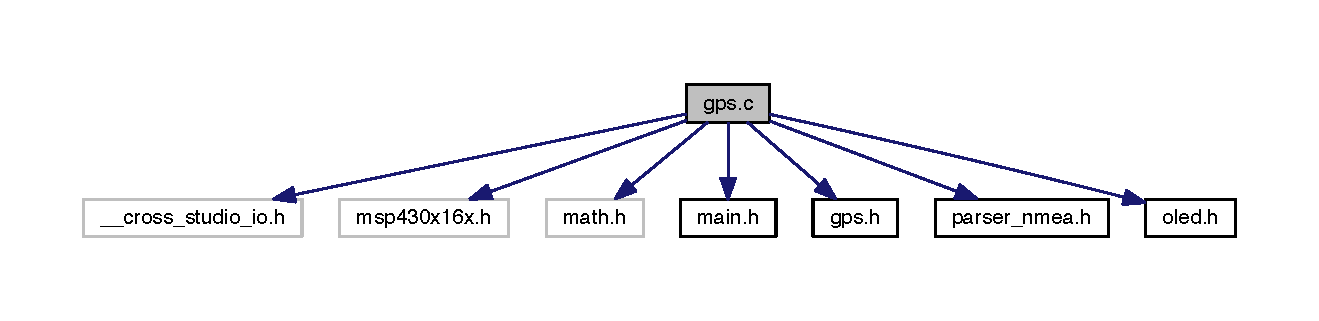
\includegraphics[width=350pt]{gps_8c__incl}
\end{center}
\end{figure}
\subsection*{Functions}
\begin{DoxyCompactItemize}
\item 
void \hyperlink{gps_8c_a1b2aba3f16e2e76c7289b7037b6efc16}{toggle\+G\+PS} (unsigned int state)
\begin{DoxyCompactList}\small\item\em Toggle G\+PS (P4.\+0, E\+N\+A\+B\+L\+E\+\_\+\+G\+PS) \end{DoxyCompactList}\item 
void \hyperlink{gps_8c_a505a87b467a4594e9bea58310c07d5b4}{toggle\+G\+P\+S\+Interrupt} (unsigned int state)
\begin{DoxyCompactList}\small\item\em Toggle G\+PS interrupt. \end{DoxyCompactList}\item 
void \hyperlink{gps_8c_af9ec31d367c0cc4a56d807765b4db0ed}{enable\+U\+S\+A\+R\+Tfor\+G\+PS} (void)\hypertarget{gps_8c_af9ec31d367c0cc4a56d807765b4db0ed}{}\label{gps_8c_af9ec31d367c0cc4a56d807765b4db0ed}

\begin{DoxyCompactList}\small\item\em Enable and config U\+S\+A\+RT for G\+PS. \end{DoxyCompactList}\item 
void \hyperlink{gps_8c_af1e989480dca39d7a385e41f529c0e98}{gps\+Send} (char $\ast$message)
\begin{DoxyCompactList}\small\item\em Send sentences to G\+PS to configure it (interrupt mode) \end{DoxyCompactList}\item 
void \hyperlink{gps_8c_a395226ecf7a4ed334cafb3f3bfd5355f}{usart0\+\_\+rx} (void)\hypertarget{gps_8c_a395226ecf7a4ed334cafb3f3bfd5355f}{}\label{gps_8c_a395226ecf7a4ed334cafb3f3bfd5355f}

\begin{DoxyCompactList}\small\item\em Receive function for G\+PS data (U\+S\+A\+R\+T0, interrupt mode) \end{DoxyCompactList}\item 
float \hyperlink{gps_8c_a678d7cc4446981494885b356815b5c7c}{calc\+Distance} (float lat1, float lon1, float lat2, float lon2)
\begin{DoxyCompactList}\small\item\em Calculate the distance between two points (Haversine formula) \end{DoxyCompactList}\item 
float \hyperlink{gps_8c_af3e32657c50564111148c55eb12ebebd}{deg2rad} (float deg)
\begin{DoxyCompactList}\small\item\em Degrees to radians converter. \end{DoxyCompactList}\end{DoxyCompactItemize}
\subsection*{Variables}
\begin{DoxyCompactItemize}
\item 
unsigned int \hyperlink{gps_8c_acc0a9ba9c05879c88bf0396f6a27a751}{data\+Valid}
\item 
\hyperlink{structgps__data}{gps\+\_\+data} \hyperlink{gps_8c_a78c92d17a8c361eab9ff753a35888f02}{G\+P\+S\+Data}
\begin{DoxyCompactList}\small\item\em Store G\+PS valid data. \end{DoxyCompactList}\end{DoxyCompactItemize}


\subsection{Detailed Description}
File containing the G\+PS functions. 

\begin{DoxyAuthor}{Author}
Gaël Foppolo (gaelfoppolo) 
\end{DoxyAuthor}


\subsection{Function Documentation}
\index{gps.\+c@{gps.\+c}!calc\+Distance@{calc\+Distance}}
\index{calc\+Distance@{calc\+Distance}!gps.\+c@{gps.\+c}}
\subsubsection[{\texorpdfstring{calc\+Distance(float lat1, float lon1, float lat2, float lon2)}{calcDistance(float lat1, float lon1, float lat2, float lon2)}}]{\setlength{\rightskip}{0pt plus 5cm}float calc\+Distance (
\begin{DoxyParamCaption}
\item[{float}]{lat1, }
\item[{float}]{lon1, }
\item[{float}]{lat2, }
\item[{float}]{lon2}
\end{DoxyParamCaption}
)}\hypertarget{gps_8c_a678d7cc4446981494885b356815b5c7c}{}\label{gps_8c_a678d7cc4446981494885b356815b5c7c}


Calculate the distance between two points (Haversine formula) 

\begin{DoxySeeAlso}{See also}
Wikipedia
\end{DoxySeeAlso}

\begin{DoxyParams}{Parameters}
{\em lat1} & The latitude of the first point \\
\hline
{\em lon1} & The longitude of the first point \\
\hline
{\em lat2} & The latitude of the second point \\
\hline
{\em lon2} & The longitude of the second point \\
\hline
\end{DoxyParams}
\begin{DoxyReturn}{Returns}
The distance (in km) 
\end{DoxyReturn}


Here is the call graph for this function\+:\nopagebreak
\begin{figure}[H]
\begin{center}
\leavevmode
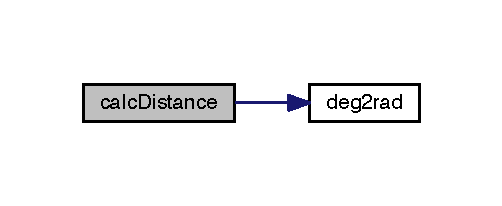
\includegraphics[width=241pt]{gps_8c_a678d7cc4446981494885b356815b5c7c_cgraph}
\end{center}
\end{figure}


\index{gps.\+c@{gps.\+c}!deg2rad@{deg2rad}}
\index{deg2rad@{deg2rad}!gps.\+c@{gps.\+c}}
\subsubsection[{\texorpdfstring{deg2rad(float deg)}{deg2rad(float deg)}}]{\setlength{\rightskip}{0pt plus 5cm}float deg2rad (
\begin{DoxyParamCaption}
\item[{float}]{deg}
\end{DoxyParamCaption}
)}\hypertarget{gps_8c_af3e32657c50564111148c55eb12ebebd}{}\label{gps_8c_af3e32657c50564111148c55eb12ebebd}


Degrees to radians converter. 


\begin{DoxyParams}{Parameters}
{\em deg} & The angle in degrees \\
\hline
\end{DoxyParams}
\begin{DoxyReturn}{Returns}
The angle in radians 
\end{DoxyReturn}


Here is the caller graph for this function\+:\nopagebreak
\begin{figure}[H]
\begin{center}
\leavevmode
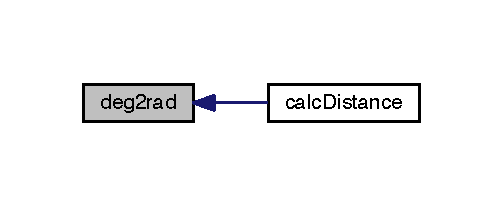
\includegraphics[width=241pt]{gps_8c_af3e32657c50564111148c55eb12ebebd_icgraph}
\end{center}
\end{figure}


\index{gps.\+c@{gps.\+c}!gps\+Send@{gps\+Send}}
\index{gps\+Send@{gps\+Send}!gps.\+c@{gps.\+c}}
\subsubsection[{\texorpdfstring{gps\+Send(char $\ast$message)}{gpsSend(char *message)}}]{\setlength{\rightskip}{0pt plus 5cm}void gps\+Send (
\begin{DoxyParamCaption}
\item[{char $\ast$}]{message}
\end{DoxyParamCaption}
)}\hypertarget{gps_8c_af1e989480dca39d7a385e41f529c0e98}{}\label{gps_8c_af1e989480dca39d7a385e41f529c0e98}


Send sentences to G\+PS to configure it (interrupt mode) 


\begin{DoxyParams}{Parameters}
{\em message} & Message to send \\
\hline
\end{DoxyParams}


Here is the caller graph for this function\+:\nopagebreak
\begin{figure}[H]
\begin{center}
\leavevmode
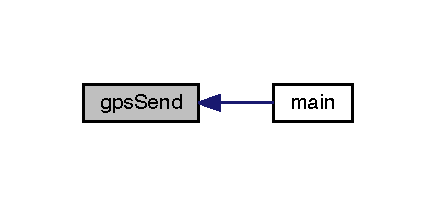
\includegraphics[width=209pt]{gps_8c_af1e989480dca39d7a385e41f529c0e98_icgraph}
\end{center}
\end{figure}


\index{gps.\+c@{gps.\+c}!toggle\+G\+PS@{toggle\+G\+PS}}
\index{toggle\+G\+PS@{toggle\+G\+PS}!gps.\+c@{gps.\+c}}
\subsubsection[{\texorpdfstring{toggle\+G\+P\+S(unsigned int state)}{toggleGPS(unsigned int state)}}]{\setlength{\rightskip}{0pt plus 5cm}void toggle\+G\+PS (
\begin{DoxyParamCaption}
\item[{unsigned int}]{state}
\end{DoxyParamCaption}
)}\hypertarget{gps_8c_a1b2aba3f16e2e76c7289b7037b6efc16}{}\label{gps_8c_a1b2aba3f16e2e76c7289b7037b6efc16}


Toggle G\+PS (P4.\+0, E\+N\+A\+B\+L\+E\+\_\+\+G\+PS) 

1 = enable, 0 = disable


\begin{DoxyParams}{Parameters}
{\em state} & The new state \\
\hline
\end{DoxyParams}


Here is the caller graph for this function\+:\nopagebreak
\begin{figure}[H]
\begin{center}
\leavevmode
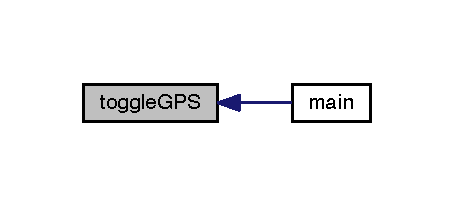
\includegraphics[width=218pt]{gps_8c_a1b2aba3f16e2e76c7289b7037b6efc16_icgraph}
\end{center}
\end{figure}


\index{gps.\+c@{gps.\+c}!toggle\+G\+P\+S\+Interrupt@{toggle\+G\+P\+S\+Interrupt}}
\index{toggle\+G\+P\+S\+Interrupt@{toggle\+G\+P\+S\+Interrupt}!gps.\+c@{gps.\+c}}
\subsubsection[{\texorpdfstring{toggle\+G\+P\+S\+Interrupt(unsigned int state)}{toggleGPSInterrupt(unsigned int state)}}]{\setlength{\rightskip}{0pt plus 5cm}void toggle\+G\+P\+S\+Interrupt (
\begin{DoxyParamCaption}
\item[{unsigned int}]{state}
\end{DoxyParamCaption}
)}\hypertarget{gps_8c_a505a87b467a4594e9bea58310c07d5b4}{}\label{gps_8c_a505a87b467a4594e9bea58310c07d5b4}


Toggle G\+PS interrupt. 

1 = interrupt enable for G\+PS, 0 = disable


\begin{DoxyParams}{Parameters}
{\em state} & The new state \\
\hline
\end{DoxyParams}


Here is the caller graph for this function\+:\nopagebreak
\begin{figure}[H]
\begin{center}
\leavevmode
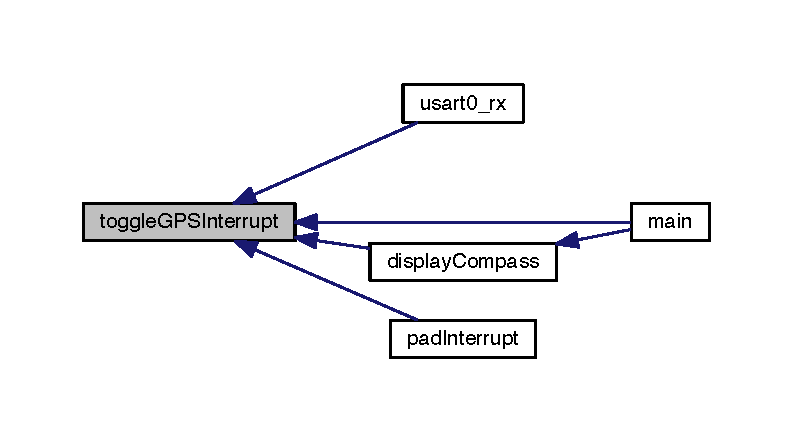
\includegraphics[width=350pt]{gps_8c_a505a87b467a4594e9bea58310c07d5b4_icgraph}
\end{center}
\end{figure}




\subsection{Variable Documentation}
\index{gps.\+c@{gps.\+c}!data\+Valid@{data\+Valid}}
\index{data\+Valid@{data\+Valid}!gps.\+c@{gps.\+c}}
\subsubsection[{\texorpdfstring{data\+Valid}{dataValid}}]{\setlength{\rightskip}{0pt plus 5cm}unsigned int data\+Valid}\hypertarget{gps_8c_acc0a9ba9c05879c88bf0396f6a27a751}{}\label{gps_8c_acc0a9ba9c05879c88bf0396f6a27a751}
Data are valid or not? \index{gps.\+c@{gps.\+c}!G\+P\+S\+Data@{G\+P\+S\+Data}}
\index{G\+P\+S\+Data@{G\+P\+S\+Data}!gps.\+c@{gps.\+c}}
\subsubsection[{\texorpdfstring{G\+P\+S\+Data}{GPSData}}]{\setlength{\rightskip}{0pt plus 5cm}{\bf gps\+\_\+data} G\+P\+S\+Data}\hypertarget{gps_8c_a78c92d17a8c361eab9ff753a35888f02}{}\label{gps_8c_a78c92d17a8c361eab9ff753a35888f02}


Store G\+PS valid data. 

Useful data received and valid. 
\hypertarget{gps_8h}{}\section{software/gps.h File Reference}
\label{gps_8h}\index{software/gps.\+h@{software/gps.\+h}}


File containing the G\+PS functions.  


This graph shows which files directly or indirectly include this file\+:\nopagebreak
\begin{figure}[H]
\begin{center}
\leavevmode
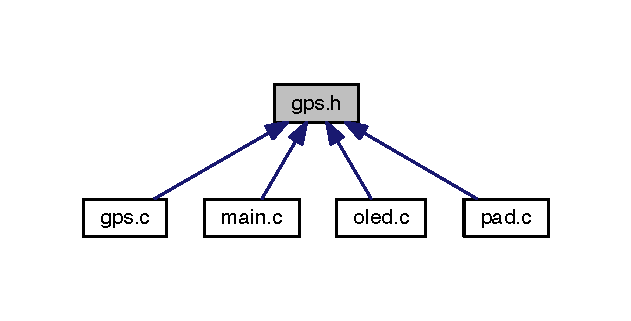
\includegraphics[width=350pt]{gps_8h__dep__incl}
\end{center}
\end{figure}
\subsection*{Data Structures}
\begin{DoxyCompactItemize}
\item 
struct \hyperlink{structgps__data}{gps\+\_\+data}
\end{DoxyCompactItemize}
\subsection*{Macros}
\begin{DoxyCompactItemize}
\item 
\#define \hyperlink{gps_8h_a62189e29f8841d050efe64f2fe1d7dc2}{N\+U\+M\+B\+E\+R\+S\+\_\+\+O\+F\+\_\+\+S\+E\+N\+T\+E\+N\+CE}~4\hypertarget{gps_8h_a62189e29f8841d050efe64f2fe1d7dc2}{}\label{gps_8h_a62189e29f8841d050efe64f2fe1d7dc2}

\begin{DoxyCompactList}\small\item\em How many sentences do we want to receive in interrupt mode. \end{DoxyCompactList}\item 
\#define \hyperlink{gps_8h_a33263b2497472563e66715b134af0f51}{N\+U\+M\+B\+E\+R\+S\+\_\+\+O\+F\+\_\+\+S\+E\+N\+T\+E\+N\+C\+E\+\_\+\+M\+AX}~10\hypertarget{gps_8h_a33263b2497472563e66715b134af0f51}{}\label{gps_8h_a33263b2497472563e66715b134af0f51}

\begin{DoxyCompactList}\small\item\em How many sentences do we want to receive in interrupt mode (M\+AX) \end{DoxyCompactList}\item 
\#define \hyperlink{gps_8h_aa4a8f077b24c13804708ef96ac8198d3}{R\+A\+T\+E\+\_\+1\+S\+EC}~\char`\"{}\$P\+M\+T\+K220,1000$\ast$1\+F\textbackslash{}r\textbackslash{}n\char`\"{}\hypertarget{gps_8h_aa4a8f077b24c13804708ef96ac8198d3}{}\label{gps_8h_aa4a8f077b24c13804708ef96ac8198d3}

\begin{DoxyCompactList}\small\item\em G\+PS emits N\+M\+EA sentences every 1 sec. \end{DoxyCompactList}\item 
\#define \hyperlink{gps_8h_afa86b5b296e8337b201d62162c436838}{R\+A\+T\+E\+\_\+2\+S\+EC}~\char`\"{}\$P\+M\+T\+K220,2000$\ast$1\+C\textbackslash{}r\textbackslash{}n\char`\"{}\hypertarget{gps_8h_afa86b5b296e8337b201d62162c436838}{}\label{gps_8h_afa86b5b296e8337b201d62162c436838}

\begin{DoxyCompactList}\small\item\em G\+PS emits N\+M\+EA sentences every 2 sec. \end{DoxyCompactList}\item 
\#define \hyperlink{gps_8h_aca173669bad7f70707b0eb4945d041c3}{R\+A\+T\+E\+\_\+5\+S\+EC}~\char`\"{}\$P\+M\+T\+K220,5000$\ast$1\+B\textbackslash{}r\textbackslash{}n\char`\"{}\hypertarget{gps_8h_aca173669bad7f70707b0eb4945d041c3}{}\label{gps_8h_aca173669bad7f70707b0eb4945d041c3}

\begin{DoxyCompactList}\small\item\em G\+PS emits N\+M\+EA sentences every 5 sec. \end{DoxyCompactList}\item 
\#define \hyperlink{gps_8h_a947e2f836c8084c7c7213380731325c3}{R\+A\+T\+E\+\_\+10\+S\+EC}~\char`\"{}\$P\+M\+T\+K220,10000$\ast$2\+F\textbackslash{}r\textbackslash{}n\char`\"{}\hypertarget{gps_8h_a947e2f836c8084c7c7213380731325c3}{}\label{gps_8h_a947e2f836c8084c7c7213380731325c3}

\begin{DoxyCompactList}\small\item\em G\+PS emits N\+M\+EA sentences every 10 sec. \end{DoxyCompactList}\item 
\#define \hyperlink{gps_8h_af51063242af2138ec23fea3e2c43f7e5}{D\+I\+S\+A\+B\+L\+E\+\_\+\+A\+LL}~\char`\"{}\$P\+M\+T\+K314,0,0,0,0,0,0,0,0,0,0,0,0,0,0,0,0,0,0,0$\ast$28\textbackslash{}r\textbackslash{}n\char`\"{}\hypertarget{gps_8h_af51063242af2138ec23fea3e2c43f7e5}{}\label{gps_8h_af51063242af2138ec23fea3e2c43f7e5}

\begin{DoxyCompactList}\small\item\em Tell the G\+PS to not send sentences. \end{DoxyCompactList}\item 
\#define \hyperlink{gps_8h_aae7dec6db750dd6745877e5c27dbd495}{T\+U\+R\+N\+\_\+\+A\+LL}~\char`\"{}\$P\+M\+T\+K314,1,1,1,1,1,1,0,0,0,0,0,0,0,0,0,0,0,0,0$\ast$28\textbackslash{}r\textbackslash{}n\char`\"{}\hypertarget{gps_8h_aae7dec6db750dd6745877e5c27dbd495}{}\label{gps_8h_aae7dec6db750dd6745877e5c27dbd495}

\begin{DoxyCompactList}\small\item\em Tell the G\+PS to send all sentences. \end{DoxyCompactList}\item 
\#define \hyperlink{gps_8h_a7c816b68ed551fafe92c39b721d32589}{G\+G\+A\+\_\+\+R\+MC}~\char`\"{}\$P\+M\+T\+K314,0,1,0,1,0,0,0,0,0,0,0,0,0,0,0,0,0,0,0$\ast$28\textbackslash{}r\textbackslash{}n\char`\"{}\hypertarget{gps_8h_a7c816b68ed551fafe92c39b721d32589}{}\label{gps_8h_a7c816b68ed551fafe92c39b721d32589}

\begin{DoxyCompactList}\small\item\em Tell the G\+PS to send G\+GA and R\+MC sentences only. \end{DoxyCompactList}\item 
\#define \hyperlink{gps_8h_a4627678760c059e78eea5cc0af96300b}{R\+M\+C\+\_\+\+O\+N\+LY}~\char`\"{}\$P\+M\+T\+K314,0,1,0,0,0,0,0,0,0,0,0,0,0,0,0,0,0,0,0$\ast$29\textbackslash{}r\textbackslash{}n\char`\"{}\hypertarget{gps_8h_a4627678760c059e78eea5cc0af96300b}{}\label{gps_8h_a4627678760c059e78eea5cc0af96300b}

\begin{DoxyCompactList}\small\item\em Tell the G\+PS to send R\+MC sentences only. \end{DoxyCompactList}\end{DoxyCompactItemize}
\subsection*{Typedefs}
\begin{DoxyCompactItemize}
\item 
typedef struct \hyperlink{structgps__data}{gps\+\_\+data} \hyperlink{gps_8h_a25c0be044aae01fe5952e72cc69be630}{gps\+\_\+data}
\end{DoxyCompactItemize}
\subsection*{Functions}
\begin{DoxyCompactItemize}
\item 
void \hyperlink{gps_8h_a1b2aba3f16e2e76c7289b7037b6efc16}{toggle\+G\+PS} (unsigned int state)
\begin{DoxyCompactList}\small\item\em Toggle G\+PS (P4.\+0, E\+N\+A\+B\+L\+E\+\_\+\+G\+PS) \end{DoxyCompactList}\item 
void \hyperlink{gps_8h_a505a87b467a4594e9bea58310c07d5b4}{toggle\+G\+P\+S\+Interrupt} (unsigned int state)
\begin{DoxyCompactList}\small\item\em Toggle G\+PS interrupt. \end{DoxyCompactList}\item 
void \hyperlink{gps_8h_af9ec31d367c0cc4a56d807765b4db0ed}{enable\+U\+S\+A\+R\+Tfor\+G\+PS} (void)\hypertarget{gps_8h_af9ec31d367c0cc4a56d807765b4db0ed}{}\label{gps_8h_af9ec31d367c0cc4a56d807765b4db0ed}

\begin{DoxyCompactList}\small\item\em Enable and config U\+S\+A\+RT for G\+PS. \end{DoxyCompactList}\item 
void \hyperlink{gps_8h_af1e989480dca39d7a385e41f529c0e98}{gps\+Send} (char $\ast$message)
\begin{DoxyCompactList}\small\item\em Send sentences to G\+PS to configure it (interrupt mode) \end{DoxyCompactList}\item 
void \hyperlink{gps_8h_a395226ecf7a4ed334cafb3f3bfd5355f}{usart0\+\_\+rx} (void)\hypertarget{gps_8h_a395226ecf7a4ed334cafb3f3bfd5355f}{}\label{gps_8h_a395226ecf7a4ed334cafb3f3bfd5355f}

\begin{DoxyCompactList}\small\item\em Receive function for G\+PS data (U\+S\+A\+R\+T0, interrupt mode) \end{DoxyCompactList}\item 
float \hyperlink{gps_8h_a678d7cc4446981494885b356815b5c7c}{calc\+Distance} (float lat1, float lon1, float lat2, float lon2)
\begin{DoxyCompactList}\small\item\em Calculate the distance between two points (Haversine formula) \end{DoxyCompactList}\item 
float \hyperlink{gps_8h_af3e32657c50564111148c55eb12ebebd}{deg2rad} (float deg)
\begin{DoxyCompactList}\small\item\em Degrees to radians converter. \end{DoxyCompactList}\end{DoxyCompactItemize}
\subsection*{Variables}
\begin{DoxyCompactItemize}
\item 
unsigned int \hyperlink{gps_8h_acc0a9ba9c05879c88bf0396f6a27a751}{data\+Valid}
\item 
struct \hyperlink{structgps__data}{gps\+\_\+data} \hyperlink{gps_8h_adb53c8db76d434b097530cca333b4d1e}{G\+P\+S\+Data}
\begin{DoxyCompactList}\small\item\em Useful data received and valid. \end{DoxyCompactList}\end{DoxyCompactItemize}


\subsection{Detailed Description}
File containing the G\+PS functions. 

\begin{DoxyAuthor}{Author}
Gaël Foppolo (gaelfoppolo) 
\end{DoxyAuthor}


\subsection{Typedef Documentation}
\index{gps.\+h@{gps.\+h}!gps\+\_\+data@{gps\+\_\+data}}
\index{gps\+\_\+data@{gps\+\_\+data}!gps.\+h@{gps.\+h}}
\subsubsection[{\texorpdfstring{gps\+\_\+data}{gps_data}}]{\setlength{\rightskip}{0pt plus 5cm}typedef struct {\bf gps\+\_\+data}  {\bf gps\+\_\+data}}\hypertarget{gps_8h_a25c0be044aae01fe5952e72cc69be630}{}\label{gps_8h_a25c0be044aae01fe5952e72cc69be630}
Structure that contains useful G\+PS data 

\subsection{Function Documentation}
\index{gps.\+h@{gps.\+h}!calc\+Distance@{calc\+Distance}}
\index{calc\+Distance@{calc\+Distance}!gps.\+h@{gps.\+h}}
\subsubsection[{\texorpdfstring{calc\+Distance(float lat1, float lon1, float lat2, float lon2)}{calcDistance(float lat1, float lon1, float lat2, float lon2)}}]{\setlength{\rightskip}{0pt plus 5cm}float calc\+Distance (
\begin{DoxyParamCaption}
\item[{float}]{lat1, }
\item[{float}]{lon1, }
\item[{float}]{lat2, }
\item[{float}]{lon2}
\end{DoxyParamCaption}
)}\hypertarget{gps_8h_a678d7cc4446981494885b356815b5c7c}{}\label{gps_8h_a678d7cc4446981494885b356815b5c7c}


Calculate the distance between two points (Haversine formula) 

\begin{DoxySeeAlso}{See also}
Wikipedia
\end{DoxySeeAlso}

\begin{DoxyParams}{Parameters}
{\em lat1} & The latitude of the first point \\
\hline
{\em lon1} & The longitude of the first point \\
\hline
{\em lat2} & The latitude of the second point \\
\hline
{\em lon2} & The longitude of the second point \\
\hline
\end{DoxyParams}
\begin{DoxyReturn}{Returns}
The distance (in km) 
\end{DoxyReturn}


Here is the call graph for this function\+:\nopagebreak
\begin{figure}[H]
\begin{center}
\leavevmode
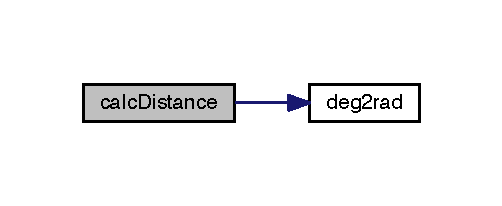
\includegraphics[width=241pt]{gps_8h_a678d7cc4446981494885b356815b5c7c_cgraph}
\end{center}
\end{figure}


\index{gps.\+h@{gps.\+h}!deg2rad@{deg2rad}}
\index{deg2rad@{deg2rad}!gps.\+h@{gps.\+h}}
\subsubsection[{\texorpdfstring{deg2rad(float deg)}{deg2rad(float deg)}}]{\setlength{\rightskip}{0pt plus 5cm}float deg2rad (
\begin{DoxyParamCaption}
\item[{float}]{deg}
\end{DoxyParamCaption}
)}\hypertarget{gps_8h_af3e32657c50564111148c55eb12ebebd}{}\label{gps_8h_af3e32657c50564111148c55eb12ebebd}


Degrees to radians converter. 


\begin{DoxyParams}{Parameters}
{\em deg} & The angle in degrees \\
\hline
\end{DoxyParams}
\begin{DoxyReturn}{Returns}
The angle in radians 
\end{DoxyReturn}


Here is the caller graph for this function\+:\nopagebreak
\begin{figure}[H]
\begin{center}
\leavevmode
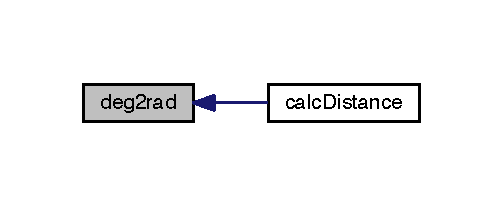
\includegraphics[width=241pt]{gps_8h_af3e32657c50564111148c55eb12ebebd_icgraph}
\end{center}
\end{figure}


\index{gps.\+h@{gps.\+h}!gps\+Send@{gps\+Send}}
\index{gps\+Send@{gps\+Send}!gps.\+h@{gps.\+h}}
\subsubsection[{\texorpdfstring{gps\+Send(char $\ast$message)}{gpsSend(char *message)}}]{\setlength{\rightskip}{0pt plus 5cm}void gps\+Send (
\begin{DoxyParamCaption}
\item[{char $\ast$}]{message}
\end{DoxyParamCaption}
)}\hypertarget{gps_8h_af1e989480dca39d7a385e41f529c0e98}{}\label{gps_8h_af1e989480dca39d7a385e41f529c0e98}


Send sentences to G\+PS to configure it (interrupt mode) 


\begin{DoxyParams}{Parameters}
{\em message} & Message to send \\
\hline
\end{DoxyParams}


Here is the caller graph for this function\+:\nopagebreak
\begin{figure}[H]
\begin{center}
\leavevmode
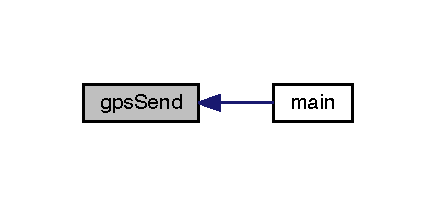
\includegraphics[width=209pt]{gps_8h_af1e989480dca39d7a385e41f529c0e98_icgraph}
\end{center}
\end{figure}


\index{gps.\+h@{gps.\+h}!toggle\+G\+PS@{toggle\+G\+PS}}
\index{toggle\+G\+PS@{toggle\+G\+PS}!gps.\+h@{gps.\+h}}
\subsubsection[{\texorpdfstring{toggle\+G\+P\+S(unsigned int state)}{toggleGPS(unsigned int state)}}]{\setlength{\rightskip}{0pt plus 5cm}void toggle\+G\+PS (
\begin{DoxyParamCaption}
\item[{unsigned int}]{state}
\end{DoxyParamCaption}
)}\hypertarget{gps_8h_a1b2aba3f16e2e76c7289b7037b6efc16}{}\label{gps_8h_a1b2aba3f16e2e76c7289b7037b6efc16}


Toggle G\+PS (P4.\+0, E\+N\+A\+B\+L\+E\+\_\+\+G\+PS) 

1 = enable, 0 = disable


\begin{DoxyParams}{Parameters}
{\em state} & The new state \\
\hline
\end{DoxyParams}


Here is the caller graph for this function\+:\nopagebreak
\begin{figure}[H]
\begin{center}
\leavevmode
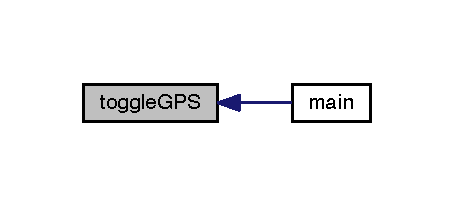
\includegraphics[width=218pt]{gps_8h_a1b2aba3f16e2e76c7289b7037b6efc16_icgraph}
\end{center}
\end{figure}


\index{gps.\+h@{gps.\+h}!toggle\+G\+P\+S\+Interrupt@{toggle\+G\+P\+S\+Interrupt}}
\index{toggle\+G\+P\+S\+Interrupt@{toggle\+G\+P\+S\+Interrupt}!gps.\+h@{gps.\+h}}
\subsubsection[{\texorpdfstring{toggle\+G\+P\+S\+Interrupt(unsigned int state)}{toggleGPSInterrupt(unsigned int state)}}]{\setlength{\rightskip}{0pt plus 5cm}void toggle\+G\+P\+S\+Interrupt (
\begin{DoxyParamCaption}
\item[{unsigned int}]{state}
\end{DoxyParamCaption}
)}\hypertarget{gps_8h_a505a87b467a4594e9bea58310c07d5b4}{}\label{gps_8h_a505a87b467a4594e9bea58310c07d5b4}


Toggle G\+PS interrupt. 

1 = interrupt enable for G\+PS, 0 = disable


\begin{DoxyParams}{Parameters}
{\em state} & The new state \\
\hline
\end{DoxyParams}


Here is the caller graph for this function\+:\nopagebreak
\begin{figure}[H]
\begin{center}
\leavevmode
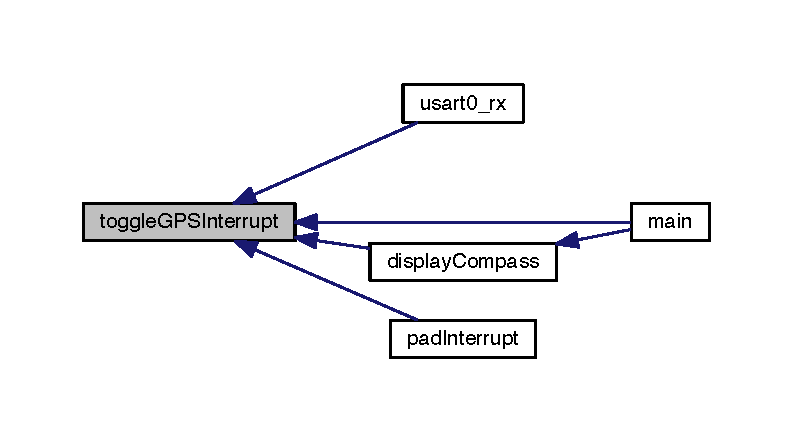
\includegraphics[width=350pt]{gps_8h_a505a87b467a4594e9bea58310c07d5b4_icgraph}
\end{center}
\end{figure}




\subsection{Variable Documentation}
\index{gps.\+h@{gps.\+h}!data\+Valid@{data\+Valid}}
\index{data\+Valid@{data\+Valid}!gps.\+h@{gps.\+h}}
\subsubsection[{\texorpdfstring{data\+Valid}{dataValid}}]{\setlength{\rightskip}{0pt plus 5cm}unsigned int data\+Valid}\hypertarget{gps_8h_acc0a9ba9c05879c88bf0396f6a27a751}{}\label{gps_8h_acc0a9ba9c05879c88bf0396f6a27a751}
Data are valid or not? \index{gps.\+h@{gps.\+h}!G\+P\+S\+Data@{G\+P\+S\+Data}}
\index{G\+P\+S\+Data@{G\+P\+S\+Data}!gps.\+h@{gps.\+h}}
\subsubsection[{\texorpdfstring{G\+P\+S\+Data}{GPSData}}]{\setlength{\rightskip}{0pt plus 5cm}struct {\bf gps\+\_\+data} G\+P\+S\+Data}\hypertarget{gps_8h_adb53c8db76d434b097530cca333b4d1e}{}\label{gps_8h_adb53c8db76d434b097530cca333b4d1e}


Useful data received and valid. 

Useful data received and valid. 
\hypertarget{led_8c}{}\section{led.\+c File Reference}
\label{led_8c}\index{led.\+c@{led.\+c}}


File containing the L\+ED functions.  


{\ttfamily \#include $<$\+\_\+\+\_\+cross\+\_\+studio\+\_\+io.\+h$>$}\\*
{\ttfamily \#include $<$msp430x16x.\+h$>$}\\*
{\ttfamily \#include \char`\"{}main.\+h\char`\"{}}\\*
{\ttfamily \#include \char`\"{}led.\+h\char`\"{}}\\*
Include dependency graph for led.\+c\+:\nopagebreak
\begin{figure}[H]
\begin{center}
\leavevmode
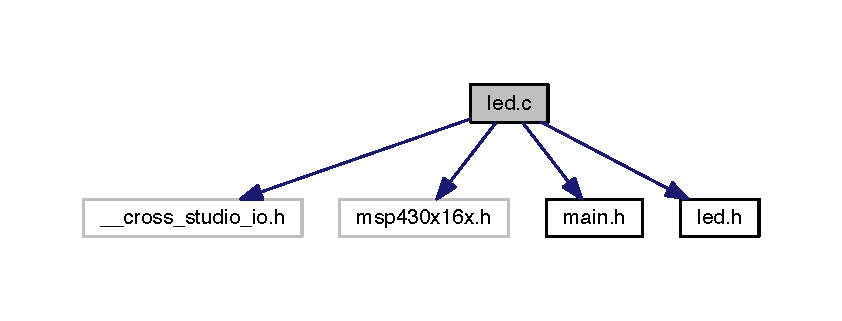
\includegraphics[width=350pt]{led_8c__incl}
\end{center}
\end{figure}
\subsection*{Functions}
\begin{DoxyCompactItemize}
\item 
void \hyperlink{led_8c_a55f6e160a6080cbf84ac546c663a0858}{init\+L\+ED} (void)
\begin{DoxyCompactList}\small\item\em Init L\+ED (P1.\+0 -\/$>$ P1.\+4) \end{DoxyCompactList}\item 
void \hyperlink{led_8c_aa5fbf250944b5272695bf3e7250bbe6e}{toggle\+L\+ED} (int n, unsigned int state, unsigned int duration)
\begin{DoxyCompactList}\small\item\em Toogle the state of the choosen L\+ED for a choosen time. \end{DoxyCompactList}\end{DoxyCompactItemize}


\subsection{Detailed Description}
File containing the L\+ED functions. 

\begin{DoxyAuthor}{Author}
Gaël Foppolo (gaelfoppolo) 
\end{DoxyAuthor}


\subsection{Function Documentation}
\index{led.\+c@{led.\+c}!init\+L\+ED@{init\+L\+ED}}
\index{init\+L\+ED@{init\+L\+ED}!led.\+c@{led.\+c}}
\subsubsection[{\texorpdfstring{init\+L\+E\+D(void)}{initLED(void)}}]{\setlength{\rightskip}{0pt plus 5cm}void init\+L\+ED (
\begin{DoxyParamCaption}
\item[{void}]{}
\end{DoxyParamCaption}
)}\hypertarget{led_8c_a55f6e160a6080cbf84ac546c663a0858}{}\label{led_8c_a55f6e160a6080cbf84ac546c663a0858}


Init L\+ED (P1.\+0 -\/$>$ P1.\+4) 

All ready to use and state cleared 

Here is the caller graph for this function\+:\nopagebreak
\begin{figure}[H]
\begin{center}
\leavevmode
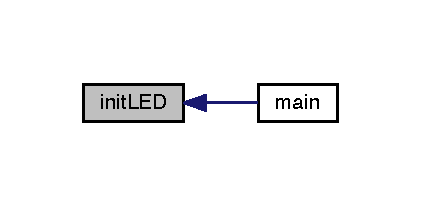
\includegraphics[width=202pt]{led_8c_a55f6e160a6080cbf84ac546c663a0858_icgraph}
\end{center}
\end{figure}


\index{led.\+c@{led.\+c}!toggle\+L\+ED@{toggle\+L\+ED}}
\index{toggle\+L\+ED@{toggle\+L\+ED}!led.\+c@{led.\+c}}
\subsubsection[{\texorpdfstring{toggle\+L\+E\+D(int n, unsigned int state, unsigned int duration)}{toggleLED(int n, unsigned int state, unsigned int duration)}}]{\setlength{\rightskip}{0pt plus 5cm}void toggle\+L\+ED (
\begin{DoxyParamCaption}
\item[{int}]{n, }
\item[{unsigned int}]{state, }
\item[{unsigned int}]{duration}
\end{DoxyParamCaption}
)}\hypertarget{led_8c_aa5fbf250944b5272695bf3e7250bbe6e}{}\label{led_8c_aa5fbf250944b5272695bf3e7250bbe6e}


Toogle the state of the choosen L\+ED for a choosen time. 

duration = 0 -\/$>$ stay in the state choosen


\begin{DoxyParams}{Parameters}
{\em n} & The L\+ED to toogle \\
\hline
{\em state} & The new state \\
\hline
{\em duration} & The time to toogle the state of the L\+ED \\
\hline
\end{DoxyParams}


Here is the call graph for this function\+:\nopagebreak
\begin{figure}[H]
\begin{center}
\leavevmode
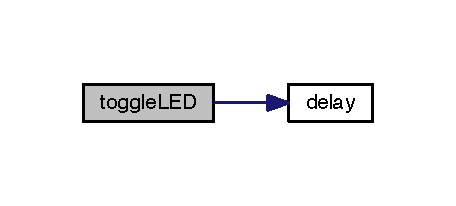
\includegraphics[width=219pt]{led_8c_aa5fbf250944b5272695bf3e7250bbe6e_cgraph}
\end{center}
\end{figure}



\hypertarget{led_8h}{}\section{led.\+h File Reference}
\label{led_8h}\index{led.\+h@{led.\+h}}


File containing the L\+ED functions.  


This graph shows which files directly or indirectly include this file\+:\nopagebreak
\begin{figure}[H]
\begin{center}
\leavevmode
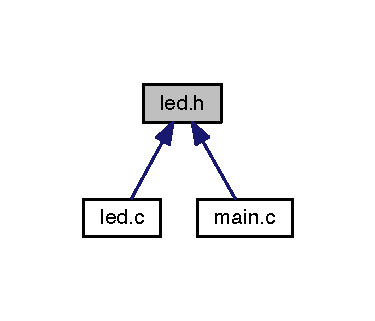
\includegraphics[width=180pt]{led_8h__dep__incl}
\end{center}
\end{figure}
\subsection*{Functions}
\begin{DoxyCompactItemize}
\item 
void \hyperlink{led_8h_a55f6e160a6080cbf84ac546c663a0858}{init\+L\+ED} (void)
\begin{DoxyCompactList}\small\item\em Init L\+ED (P1.\+0 -\/$>$ P1.\+4) \end{DoxyCompactList}\item 
void \hyperlink{led_8h_aa5fbf250944b5272695bf3e7250bbe6e}{toggle\+L\+ED} (int n, unsigned int state, unsigned int duration)
\begin{DoxyCompactList}\small\item\em Toogle the state of the choosen L\+ED for a choosen time. \end{DoxyCompactList}\end{DoxyCompactItemize}


\subsection{Detailed Description}
File containing the L\+ED functions. 

\begin{DoxyAuthor}{Author}
Gaël Foppolo (gaelfoppolo) 
\end{DoxyAuthor}


\subsection{Function Documentation}
\index{led.\+h@{led.\+h}!init\+L\+ED@{init\+L\+ED}}
\index{init\+L\+ED@{init\+L\+ED}!led.\+h@{led.\+h}}
\subsubsection[{\texorpdfstring{init\+L\+E\+D(void)}{initLED(void)}}]{\setlength{\rightskip}{0pt plus 5cm}void init\+L\+ED (
\begin{DoxyParamCaption}
\item[{void}]{}
\end{DoxyParamCaption}
)}\hypertarget{led_8h_a55f6e160a6080cbf84ac546c663a0858}{}\label{led_8h_a55f6e160a6080cbf84ac546c663a0858}


Init L\+ED (P1.\+0 -\/$>$ P1.\+4) 

All ready to use and state cleared 

Here is the caller graph for this function\+:\nopagebreak
\begin{figure}[H]
\begin{center}
\leavevmode
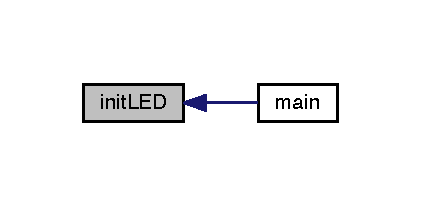
\includegraphics[width=202pt]{led_8h_a55f6e160a6080cbf84ac546c663a0858_icgraph}
\end{center}
\end{figure}


\index{led.\+h@{led.\+h}!toggle\+L\+ED@{toggle\+L\+ED}}
\index{toggle\+L\+ED@{toggle\+L\+ED}!led.\+h@{led.\+h}}
\subsubsection[{\texorpdfstring{toggle\+L\+E\+D(int n, unsigned int state, unsigned int duration)}{toggleLED(int n, unsigned int state, unsigned int duration)}}]{\setlength{\rightskip}{0pt plus 5cm}void toggle\+L\+ED (
\begin{DoxyParamCaption}
\item[{int}]{n, }
\item[{unsigned int}]{state, }
\item[{unsigned int}]{duration}
\end{DoxyParamCaption}
)}\hypertarget{led_8h_aa5fbf250944b5272695bf3e7250bbe6e}{}\label{led_8h_aa5fbf250944b5272695bf3e7250bbe6e}


Toogle the state of the choosen L\+ED for a choosen time. 

duration = 0 -\/$>$ stay in the state choosen


\begin{DoxyParams}{Parameters}
{\em n} & The L\+ED to toogle \\
\hline
{\em state} & The new state \\
\hline
{\em duration} & The time to toogle the state of the L\+ED \\
\hline
\end{DoxyParams}


Here is the call graph for this function\+:\nopagebreak
\begin{figure}[H]
\begin{center}
\leavevmode
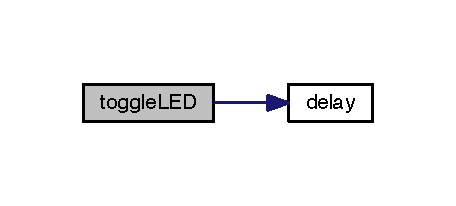
\includegraphics[width=219pt]{led_8h_aa5fbf250944b5272695bf3e7250bbe6e_cgraph}
\end{center}
\end{figure}



\hypertarget{main_8c}{}\section{software/main.c File Reference}
\label{main_8c}\index{software/main.\+c@{software/main.\+c}}


File containing the main functions.  


{\ttfamily \#include $<$\+\_\+\+\_\+cross\+\_\+studio\+\_\+io.\+h$>$}\\*
{\ttfamily \#include $<$msp430x16x.\+h$>$}\\*
{\ttfamily \#include \char`\"{}main.\+h\char`\"{}}\\*
{\ttfamily \#include \char`\"{}led.\+h\char`\"{}}\\*
{\ttfamily \#include \char`\"{}pad.\+h\char`\"{}}\\*
{\ttfamily \#include \char`\"{}gps.\+h\char`\"{}}\\*
{\ttfamily \#include \char`\"{}parser\+\_\+nmea.\+h\char`\"{}}\\*
{\ttfamily \#include \char`\"{}oled.\+h\char`\"{}}\\*
Include dependency graph for main.\+c\+:\nopagebreak
\begin{figure}[H]
\begin{center}
\leavevmode
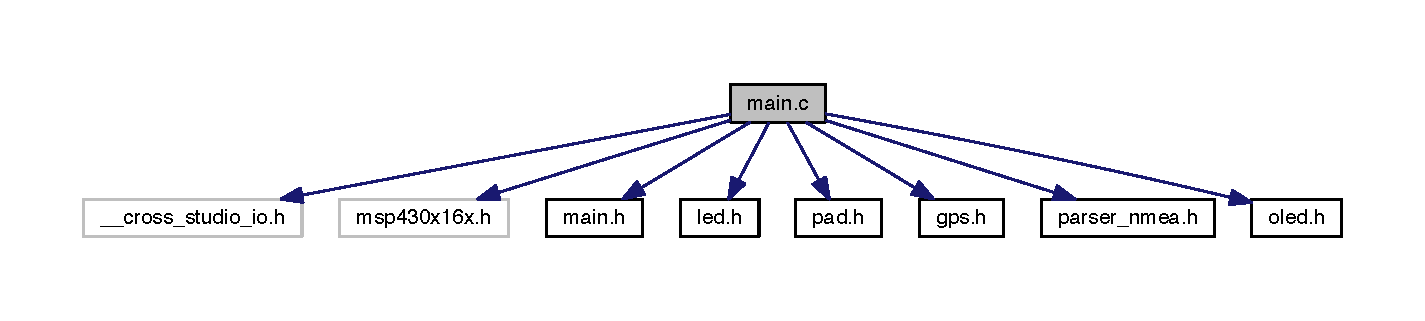
\includegraphics[width=350pt]{main_8c__incl}
\end{center}
\end{figure}
\subsection*{Functions}
\begin{DoxyCompactItemize}
\item 
void \hyperlink{main_8c_a6288eba0f8e8ad3ab1544ad731eb7667}{main} (void)
\item 
void \hyperlink{main_8c_a3bdf7d859d6f82917867c2c46f30dc21}{toggle\+Communication} (unsigned int state)
\begin{DoxyCompactList}\small\item\em Toogle the communication (P4.\+2, C\+M\+D\+\_\+\+S\+W\+I\+T\+CH) \end{DoxyCompactList}\item 
void \hyperlink{main_8c_a212def190511ade7d26638b0e25b9c2f}{configure\+Clock} (void)\hypertarget{main_8c_a212def190511ade7d26638b0e25b9c2f}{}\label{main_8c_a212def190511ade7d26638b0e25b9c2f}

\begin{DoxyCompactList}\small\item\em Configure the external clock. \end{DoxyCompactList}\item 
void \hyperlink{main_8c_acffe3bab504db5ace701416e1e400b5a}{delay} (float x)
\begin{DoxyCompactList}\small\item\em Wait for x sec. \end{DoxyCompactList}\end{DoxyCompactItemize}
\subsection*{Variables}
\begin{DoxyCompactItemize}
\item 
unsigned int \hyperlink{main_8c_ada9defc72bd97cedc77a270447a216c4}{mode\+Selected}
\end{DoxyCompactItemize}


\subsection{Detailed Description}
File containing the main functions. 

\begin{DoxyAuthor}{Author}
Gaël Foppolo (gaelfoppolo) 
\end{DoxyAuthor}


\subsection{Function Documentation}
\index{main.\+c@{main.\+c}!delay@{delay}}
\index{delay@{delay}!main.\+c@{main.\+c}}
\subsubsection[{\texorpdfstring{delay(float x)}{delay(float x)}}]{\setlength{\rightskip}{0pt plus 5cm}void delay (
\begin{DoxyParamCaption}
\item[{float}]{x}
\end{DoxyParamCaption}
)}\hypertarget{main_8c_acffe3bab504db5ace701416e1e400b5a}{}\label{main_8c_acffe3bab504db5ace701416e1e400b5a}


Wait for x sec. 


\begin{DoxyParams}{Parameters}
{\em x} & The time to wait (in sec $\sim$) \\
\hline
\end{DoxyParams}


Here is the caller graph for this function\+:\nopagebreak
\begin{figure}[H]
\begin{center}
\leavevmode
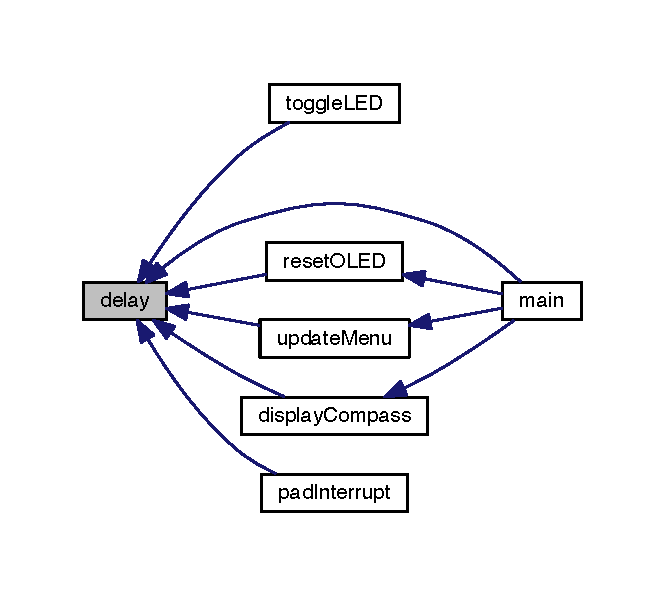
\includegraphics[width=319pt]{main_8c_acffe3bab504db5ace701416e1e400b5a_icgraph}
\end{center}
\end{figure}


\index{main.\+c@{main.\+c}!main@{main}}
\index{main@{main}!main.\+c@{main.\+c}}
\subsubsection[{\texorpdfstring{main(void)}{main(void)}}]{\setlength{\rightskip}{0pt plus 5cm}void main (
\begin{DoxyParamCaption}
\item[{void}]{}
\end{DoxyParamCaption}
)}\hypertarget{main_8c_a6288eba0f8e8ad3ab1544ad731eb7667}{}\label{main_8c_a6288eba0f8e8ad3ab1544ad731eb7667}
Menu entry point

Compass entry point

Navigation entry point

Record entry point

Shutdown entry point

Here is the call graph for this function\+:\nopagebreak
\begin{figure}[H]
\begin{center}
\leavevmode
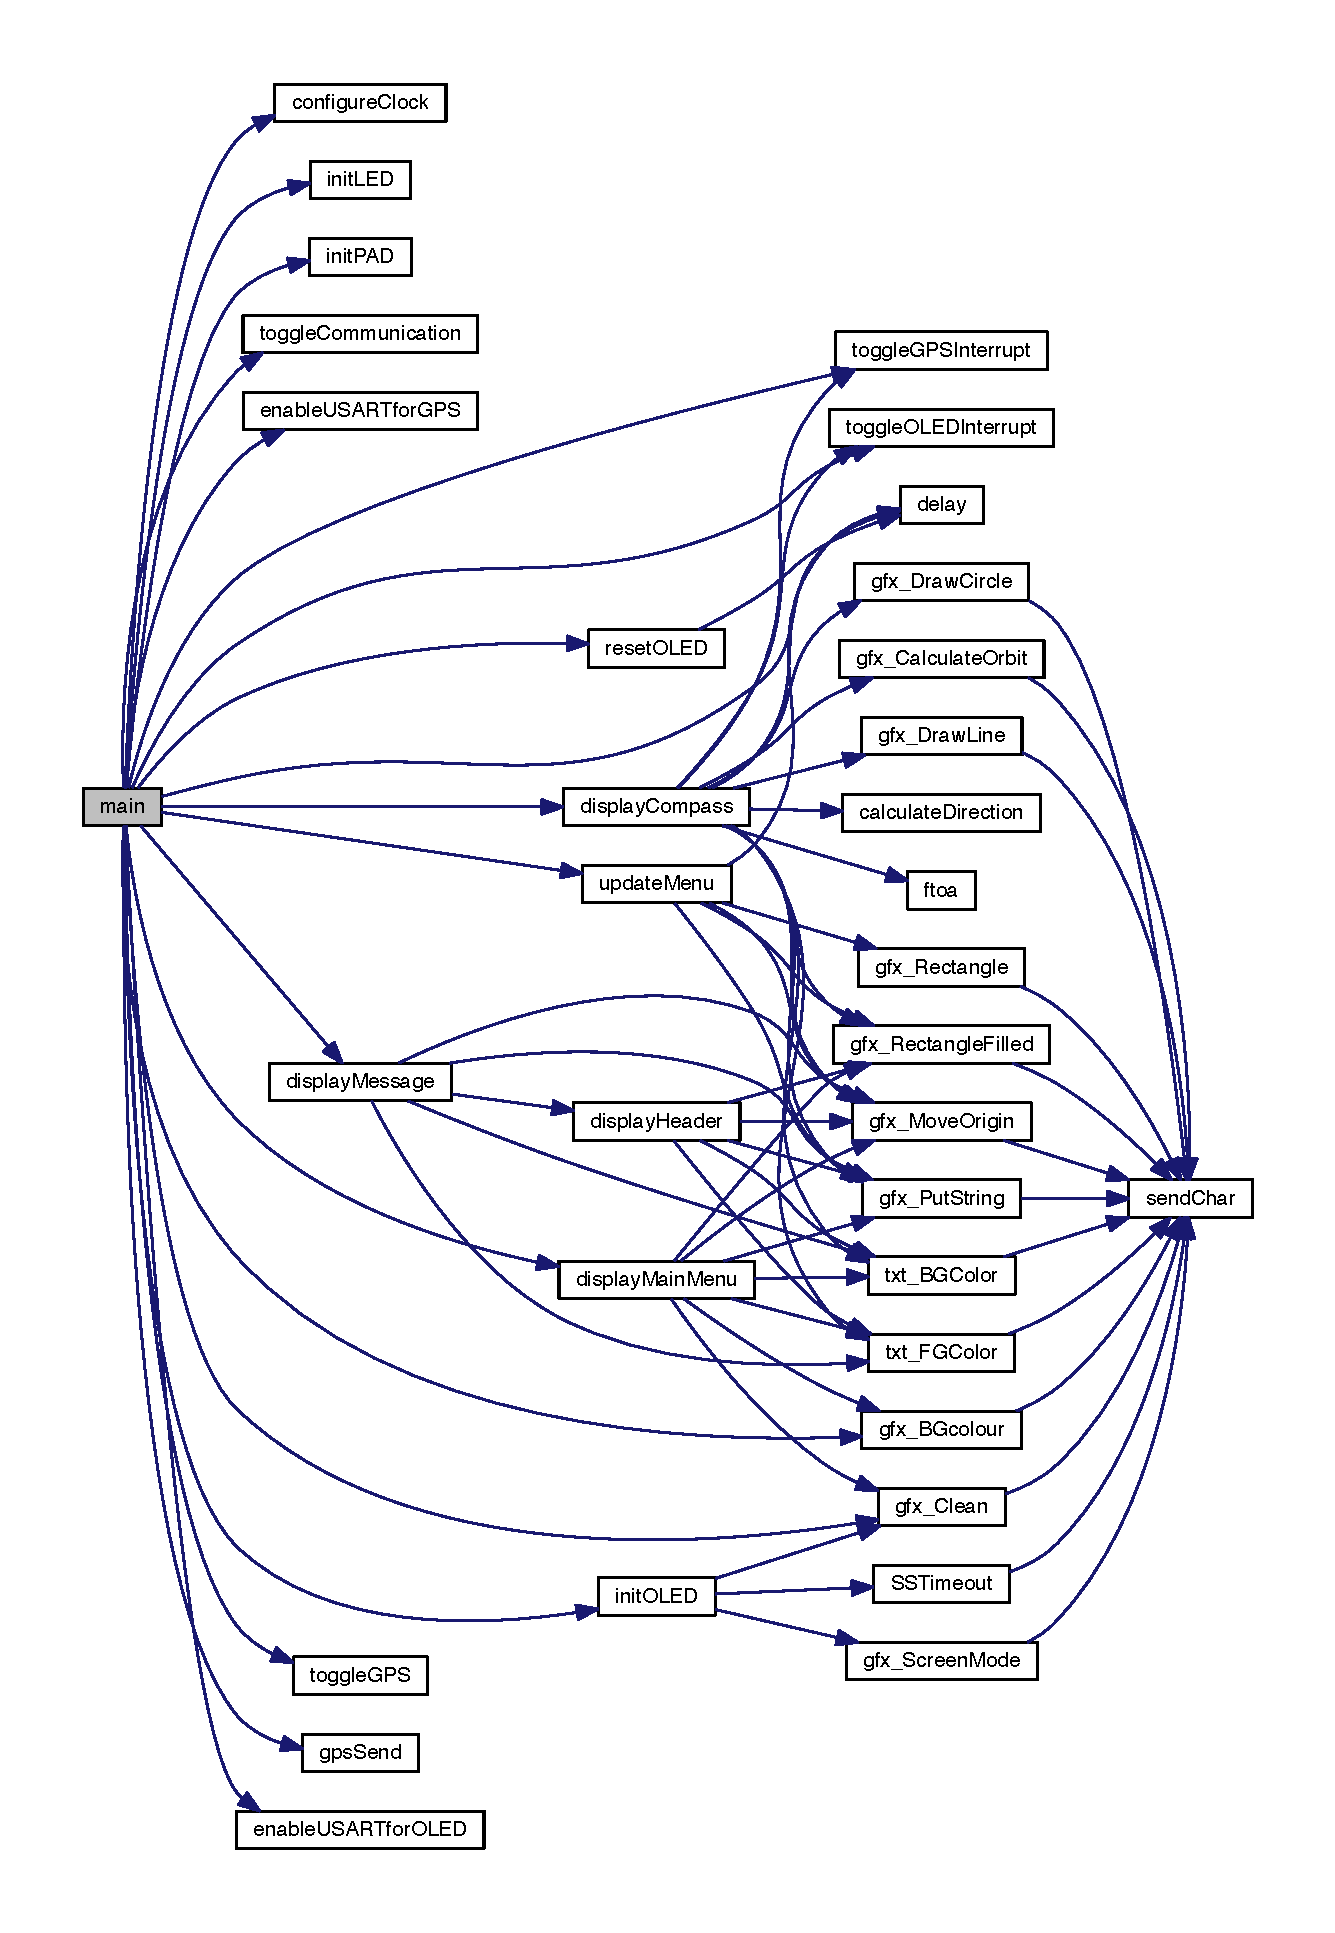
\includegraphics[width=350pt]{main_8c_a6288eba0f8e8ad3ab1544ad731eb7667_cgraph}
\end{center}
\end{figure}


\index{main.\+c@{main.\+c}!toggle\+Communication@{toggle\+Communication}}
\index{toggle\+Communication@{toggle\+Communication}!main.\+c@{main.\+c}}
\subsubsection[{\texorpdfstring{toggle\+Communication(unsigned int state)}{toggleCommunication(unsigned int state)}}]{\setlength{\rightskip}{0pt plus 5cm}void toggle\+Communication (
\begin{DoxyParamCaption}
\item[{unsigned int}]{state}
\end{DoxyParamCaption}
)}\hypertarget{main_8c_a3bdf7d859d6f82917867c2c46f30dc21}{}\label{main_8c_a3bdf7d859d6f82917867c2c46f30dc21}


Toogle the communication (P4.\+2, C\+M\+D\+\_\+\+S\+W\+I\+T\+CH) 

1 = U\+SB, 0 = G\+PS


\begin{DoxyParams}{Parameters}
{\em state} & The new state \\
\hline
\end{DoxyParams}


Here is the caller graph for this function\+:\nopagebreak
\begin{figure}[H]
\begin{center}
\leavevmode
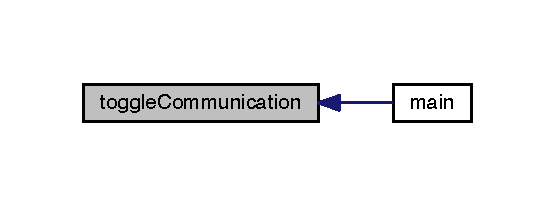
\includegraphics[width=266pt]{main_8c_a3bdf7d859d6f82917867c2c46f30dc21_icgraph}
\end{center}
\end{figure}




\subsection{Variable Documentation}
\index{main.\+c@{main.\+c}!mode\+Selected@{mode\+Selected}}
\index{mode\+Selected@{mode\+Selected}!main.\+c@{main.\+c}}
\subsubsection[{\texorpdfstring{mode\+Selected}{modeSelected}}]{\setlength{\rightskip}{0pt plus 5cm}unsigned int mode\+Selected}\hypertarget{main_8c_ada9defc72bd97cedc77a270447a216c4}{}\label{main_8c_ada9defc72bd97cedc77a270447a216c4}
Mode selected by the user, \begin{DoxySeeAlso}{See also}
\hyperlink{main_8h_a6619a470224c650b80bb6b9889f77ae6}{M\+\_\+\+M\+E\+NU}, etc. 
\end{DoxySeeAlso}

\hypertarget{main_8h}{}\section{main.\+h File Reference}
\label{main_8h}\index{main.\+h@{main.\+h}}


File containing the main functions.  


This graph shows which files directly or indirectly include this file\+:\nopagebreak
\begin{figure}[H]
\begin{center}
\leavevmode
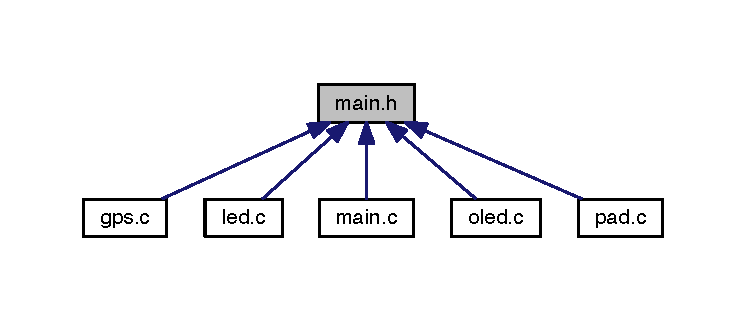
\includegraphics[width=350pt]{main_8h__dep__incl}
\end{center}
\end{figure}
\subsection*{Macros}
\begin{DoxyCompactItemize}
\item 
\#define \hyperlink{main_8h_a6619a470224c650b80bb6b9889f77ae6}{M\+\_\+\+M\+E\+NU}~0\hypertarget{main_8h_a6619a470224c650b80bb6b9889f77ae6}{}\label{main_8h_a6619a470224c650b80bb6b9889f77ae6}

\begin{DoxyCompactList}\small\item\em Mode menu. \end{DoxyCompactList}\item 
\#define \hyperlink{main_8h_a659ec114bf4c4889bbffb169a7e5f42e}{M\+\_\+\+C\+O\+M\+P\+A\+SS}~1\hypertarget{main_8h_a659ec114bf4c4889bbffb169a7e5f42e}{}\label{main_8h_a659ec114bf4c4889bbffb169a7e5f42e}

\begin{DoxyCompactList}\small\item\em Mode compass. \end{DoxyCompactList}\item 
\#define \hyperlink{main_8h_a030e6bed762d586555141f355d6ee317}{M\+\_\+\+N\+A\+V\+IG}~2\hypertarget{main_8h_a030e6bed762d586555141f355d6ee317}{}\label{main_8h_a030e6bed762d586555141f355d6ee317}

\begin{DoxyCompactList}\small\item\em Mode navigation. \end{DoxyCompactList}\item 
\#define \hyperlink{main_8h_ad3685a419333439a4814824f419c02ad}{M\+\_\+\+R\+E\+C\+O\+RD}~3\hypertarget{main_8h_ad3685a419333439a4814824f419c02ad}{}\label{main_8h_ad3685a419333439a4814824f419c02ad}

\begin{DoxyCompactList}\small\item\em Mode record. \end{DoxyCompactList}\item 
\#define \hyperlink{main_8h_a701e1b69a50830b2805557c7d5bc33e7}{M\+\_\+\+S\+H\+U\+T\+D\+O\+WN}~4\hypertarget{main_8h_a701e1b69a50830b2805557c7d5bc33e7}{}\label{main_8h_a701e1b69a50830b2805557c7d5bc33e7}

\begin{DoxyCompactList}\small\item\em Mode shutdown. \end{DoxyCompactList}\item 
\#define \hyperlink{main_8h_a03281adb3dbf8948714218169120930c}{C\+O\+M\+M\+\_\+\+G\+PS}~0\hypertarget{main_8h_a03281adb3dbf8948714218169120930c}{}\label{main_8h_a03281adb3dbf8948714218169120930c}

\begin{DoxyCompactList}\small\item\em Communication with G\+PS module. \end{DoxyCompactList}\item 
\#define \hyperlink{main_8h_a043966a31f1418c09b45f9b6d6af6a14}{C\+O\+M\+M\+\_\+\+U\+SB}~1\hypertarget{main_8h_a043966a31f1418c09b45f9b6d6af6a14}{}\label{main_8h_a043966a31f1418c09b45f9b6d6af6a14}

\begin{DoxyCompactList}\small\item\em Communication with U\+SB. \end{DoxyCompactList}\item 
\#define \hyperlink{main_8h_a7ebc9a785e5ab85457c98595aac81589}{Y\+ES}~1\hypertarget{main_8h_a7ebc9a785e5ab85457c98595aac81589}{}\label{main_8h_a7ebc9a785e5ab85457c98595aac81589}

\begin{DoxyCompactList}\small\item\em Y\+ES. \end{DoxyCompactList}\item 
\#define \hyperlink{main_8h_a996bde01ecac342918f0a2c4e7ce7bd5}{NO}~0\hypertarget{main_8h_a996bde01ecac342918f0a2c4e7ce7bd5}{}\label{main_8h_a996bde01ecac342918f0a2c4e7ce7bd5}

\begin{DoxyCompactList}\small\item\em NO. \end{DoxyCompactList}\end{DoxyCompactItemize}
\subsection*{Functions}
\begin{DoxyCompactItemize}
\item 
void \hyperlink{main_8h_a212def190511ade7d26638b0e25b9c2f}{configure\+Clock} (void)\hypertarget{main_8h_a212def190511ade7d26638b0e25b9c2f}{}\label{main_8h_a212def190511ade7d26638b0e25b9c2f}

\begin{DoxyCompactList}\small\item\em Configure the external clock. \end{DoxyCompactList}\item 
void \hyperlink{main_8h_a3bdf7d859d6f82917867c2c46f30dc21}{toggle\+Communication} (unsigned int state)
\begin{DoxyCompactList}\small\item\em Toogle the communication (P4.\+2, C\+M\+D\+\_\+\+S\+W\+I\+T\+CH) \end{DoxyCompactList}\item 
void \hyperlink{main_8h_acffe3bab504db5ace701416e1e400b5a}{delay} (float x)
\begin{DoxyCompactList}\small\item\em Wait for x sec. \end{DoxyCompactList}\end{DoxyCompactItemize}
\subsection*{Variables}
\begin{DoxyCompactItemize}
\item 
unsigned int \hyperlink{main_8h_ada9defc72bd97cedc77a270447a216c4}{mode\+Selected}
\end{DoxyCompactItemize}


\subsection{Detailed Description}
File containing the main functions. 

\begin{DoxyAuthor}{Author}
Gaël Foppolo (gaelfoppolo) 
\end{DoxyAuthor}


\subsection{Function Documentation}
\index{main.\+h@{main.\+h}!delay@{delay}}
\index{delay@{delay}!main.\+h@{main.\+h}}
\subsubsection[{\texorpdfstring{delay(float x)}{delay(float x)}}]{\setlength{\rightskip}{0pt plus 5cm}void delay (
\begin{DoxyParamCaption}
\item[{float}]{x}
\end{DoxyParamCaption}
)}\hypertarget{main_8h_acffe3bab504db5ace701416e1e400b5a}{}\label{main_8h_acffe3bab504db5ace701416e1e400b5a}


Wait for x sec. 


\begin{DoxyParams}{Parameters}
{\em x} & The time to wait (in sec $\sim$) \\
\hline
\end{DoxyParams}


Here is the caller graph for this function\+:\nopagebreak
\begin{figure}[H]
\begin{center}
\leavevmode
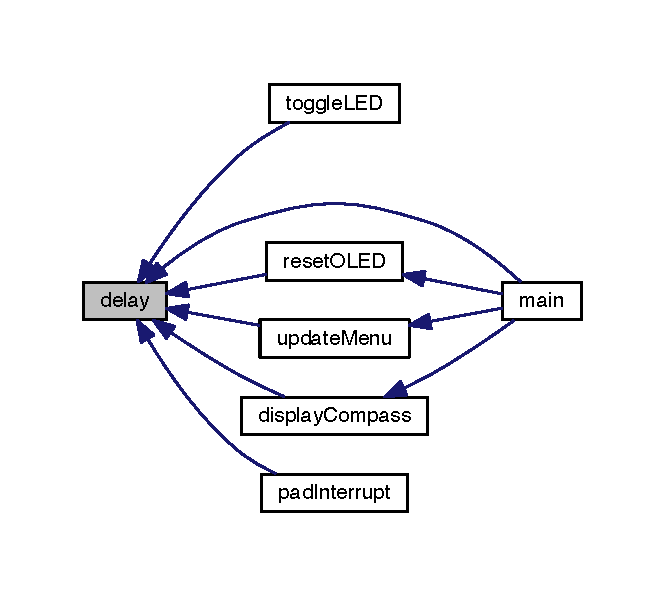
\includegraphics[width=319pt]{main_8h_acffe3bab504db5ace701416e1e400b5a_icgraph}
\end{center}
\end{figure}


\index{main.\+h@{main.\+h}!toggle\+Communication@{toggle\+Communication}}
\index{toggle\+Communication@{toggle\+Communication}!main.\+h@{main.\+h}}
\subsubsection[{\texorpdfstring{toggle\+Communication(unsigned int state)}{toggleCommunication(unsigned int state)}}]{\setlength{\rightskip}{0pt plus 5cm}void toggle\+Communication (
\begin{DoxyParamCaption}
\item[{unsigned int}]{state}
\end{DoxyParamCaption}
)}\hypertarget{main_8h_a3bdf7d859d6f82917867c2c46f30dc21}{}\label{main_8h_a3bdf7d859d6f82917867c2c46f30dc21}


Toogle the communication (P4.\+2, C\+M\+D\+\_\+\+S\+W\+I\+T\+CH) 

1 = U\+SB, 0 = G\+PS


\begin{DoxyParams}{Parameters}
{\em state} & The new state \\
\hline
\end{DoxyParams}


Here is the caller graph for this function\+:\nopagebreak
\begin{figure}[H]
\begin{center}
\leavevmode
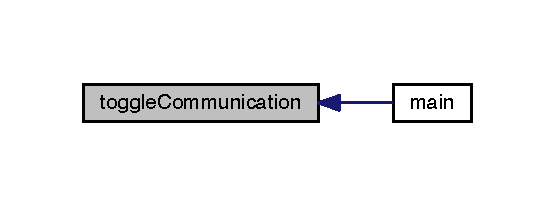
\includegraphics[width=266pt]{main_8h_a3bdf7d859d6f82917867c2c46f30dc21_icgraph}
\end{center}
\end{figure}




\subsection{Variable Documentation}
\index{main.\+h@{main.\+h}!mode\+Selected@{mode\+Selected}}
\index{mode\+Selected@{mode\+Selected}!main.\+h@{main.\+h}}
\subsubsection[{\texorpdfstring{mode\+Selected}{modeSelected}}]{\setlength{\rightskip}{0pt plus 5cm}unsigned int mode\+Selected}\hypertarget{main_8h_ada9defc72bd97cedc77a270447a216c4}{}\label{main_8h_ada9defc72bd97cedc77a270447a216c4}
Mode selected by the user, \begin{DoxySeeAlso}{See also}
\hyperlink{main_8h_a6619a470224c650b80bb6b9889f77ae6}{M\+\_\+\+M\+E\+NU}, etc. 
\end{DoxySeeAlso}

\hypertarget{oled_8c}{}\section{software/oled.c File Reference}
\label{oled_8c}\index{software/oled.\+c@{software/oled.\+c}}


File containing the O\+L\+ED functions.  


{\ttfamily \#include $<$\+\_\+\+\_\+cross\+\_\+studio\+\_\+io.\+h$>$}\\*
{\ttfamily \#include $<$msp430x16x.\+h$>$}\\*
{\ttfamily \#include $<$stdlib.\+h$>$}\\*
{\ttfamily \#include \char`\"{}main.\+h\char`\"{}}\\*
{\ttfamily \#include \char`\"{}oled.\+h\char`\"{}}\\*
{\ttfamily \#include \char`\"{}pad.\+h\char`\"{}}\\*
{\ttfamily \#include \char`\"{}gps.\+h\char`\"{}}\\*
Include dependency graph for oled.\+c\+:\nopagebreak
\begin{figure}[H]
\begin{center}
\leavevmode
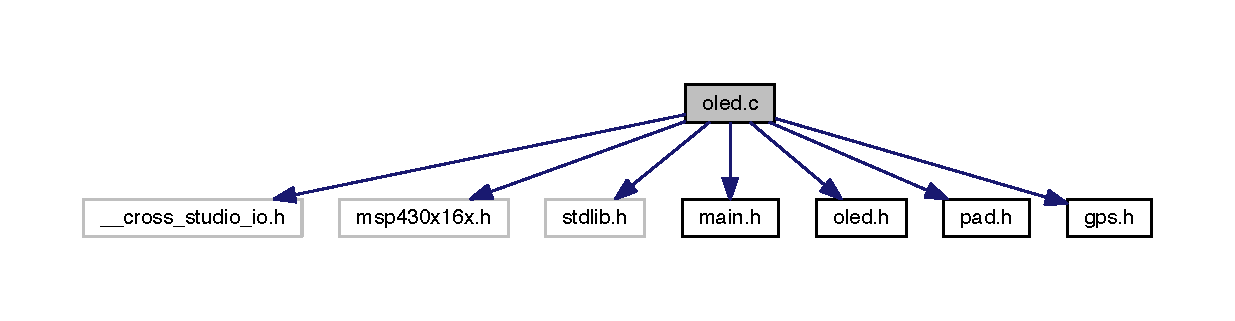
\includegraphics[width=350pt]{oled_8c__incl}
\end{center}
\end{figure}
\subsection*{Functions}
\begin{DoxyCompactItemize}
\item 
void \hyperlink{oled_8c_a69b7a13db4960f32e18281ad370f6143}{enable\+U\+S\+A\+R\+Tfor\+O\+L\+ED} (void)\hypertarget{oled_8c_a69b7a13db4960f32e18281ad370f6143}{}\label{oled_8c_a69b7a13db4960f32e18281ad370f6143}

\begin{DoxyCompactList}\small\item\em Enable and config U\+S\+A\+RT for O\+L\+ED. \end{DoxyCompactList}\item 
void \hyperlink{oled_8c_a62e9d5c0bd67eb6f17310eff7234c78b}{reset\+O\+L\+ED} ()\hypertarget{oled_8c_a62e9d5c0bd67eb6f17310eff7234c78b}{}\label{oled_8c_a62e9d5c0bd67eb6f17310eff7234c78b}

\begin{DoxyCompactList}\small\item\em Reset O\+L\+ED. \end{DoxyCompactList}\item 
void \hyperlink{oled_8c_a458006637c584f6db260748e25615708}{toggle\+O\+L\+E\+D\+Interrupt} (unsigned int state)
\begin{DoxyCompactList}\small\item\em Toggle O\+L\+ED interrupt. \end{DoxyCompactList}\item 
void \hyperlink{oled_8c_a34fe4d307e88a437023d37e3d2f39526}{send\+Char} (int c)
\begin{DoxyCompactList}\small\item\em Send char. \end{DoxyCompactList}\item 
void \hyperlink{oled_8c_acee6308d68c07654cc8857399eab9c21}{usart1\+\_\+rx} (void)\hypertarget{oled_8c_acee6308d68c07654cc8857399eab9c21}{}\label{oled_8c_acee6308d68c07654cc8857399eab9c21}

\begin{DoxyCompactList}\small\item\em Receive function for O\+L\+ED data (U\+S\+A\+R\+T1, interrupt mode) \end{DoxyCompactList}\item 
void \hyperlink{oled_8c_a5c1460e4de41069ab3e1e2577ba0e6e5}{gfx\+\_\+\+Clean} ()\hypertarget{oled_8c_a5c1460e4de41069ab3e1e2577ba0e6e5}{}\label{oled_8c_a5c1460e4de41069ab3e1e2577ba0e6e5}

\begin{DoxyCompactList}\small\item\em Clean the screen. \end{DoxyCompactList}\item 
void \hyperlink{oled_8c_a683fe37084d4bf81ec41bb048bb2d82d}{gfx\+\_\+\+B\+Gcolour} (int color)
\begin{DoxyCompactList}\small\item\em Set the background color. \end{DoxyCompactList}\item 
void \hyperlink{oled_8c_a032ab79d797b2c886854fb9044787bf4}{gfx\+\_\+\+Put\+String} (char $\ast$string)
\begin{DoxyCompactList}\small\item\em Put a string on the screen. \end{DoxyCompactList}\item 
void \hyperlink{oled_8c_a9ba037ec2bdfd47757f59d44979d6112}{gfx\+\_\+\+Rectangle\+Filled} (int x1, int y1, int x2, int y2, int color)
\begin{DoxyCompactList}\small\item\em Draw a rectangle filled with a color. \end{DoxyCompactList}\item 
void \hyperlink{oled_8c_ac7997c7454ff66e4662893fa8bc03512}{S\+S\+Timeout} (int t)
\begin{DoxyCompactList}\small\item\em Screensave mode. \end{DoxyCompactList}\item 
void \hyperlink{oled_8c_a51a164549510400e0dc556006c4c3b93}{gfx\+\_\+\+Calculate\+Orbit} (int angle, int distance, int $\ast$x, int $\ast$y)
\begin{DoxyCompactList}\small\item\em Calculate the (x,y) pos (orbit) from angle and distance. \end{DoxyCompactList}\item 
void \hyperlink{oled_8c_ab413c7645cf3692382fd74dadedb2235}{gfx\+\_\+\+Draw\+Circle} (int x, int y, int radius, int color)
\begin{DoxyCompactList}\small\item\em Draw a circle. \end{DoxyCompactList}\item 
void \hyperlink{oled_8c_a7ba83efb69401ec85f46b0f2104f892d}{gfx\+\_\+\+Draw\+Line} (int x1, int y1, int x2, int y2, int color)
\begin{DoxyCompactList}\small\item\em Draw a line. \end{DoxyCompactList}\item 
void \hyperlink{oled_8c_ac48acba04e41e0ece792c0df7baef052}{gfx\+\_\+\+Move\+Origin} (int x, int y)
\begin{DoxyCompactList}\small\item\em Move to origin to a position. \end{DoxyCompactList}\item 
void \hyperlink{oled_8c_a28c8c6d46aaa97ad945248a983f2f7d0}{gfx\+\_\+\+Screen\+Mode} (int mode)
\begin{DoxyCompactList}\small\item\em Screen mode (portrait/landscape) \end{DoxyCompactList}\item 
void \hyperlink{oled_8c_a1ad10b8c9c7f57a38615788ef00adbfd}{txt\+\_\+\+F\+G\+Color} (int color)
\begin{DoxyCompactList}\small\item\em Set the text color. \end{DoxyCompactList}\item 
void \hyperlink{oled_8c_ad673132fcf81110f70f687c441d2c218}{txt\+\_\+\+B\+G\+Color} (int color)
\begin{DoxyCompactList}\small\item\em Set the text background color. \end{DoxyCompactList}\item 
void \hyperlink{oled_8c_a0620772fba9259723deac070a4910d34}{set\+Baud\+Rate} ()\hypertarget{oled_8c_a0620772fba9259723deac070a4910d34}{}\label{oled_8c_a0620772fba9259723deac070a4910d34}

\begin{DoxyCompactList}\small\item\em Set the baud rate. \end{DoxyCompactList}\item 
void \hyperlink{oled_8c_a7bf734443a53e38b4afa062783296d90}{gfx\+\_\+\+Rectangle} (int x1, int y1, int x2, int y2, int color)
\begin{DoxyCompactList}\small\item\em Draw a rectangle. \end{DoxyCompactList}\item 
void \hyperlink{oled_8c_a9f77c9a0e006b4b9798d3ddc93e5c020}{txt\+\_\+\+Width} (int multi)
\begin{DoxyCompactList}\small\item\em Set the width of the text. \end{DoxyCompactList}\item 
void \hyperlink{oled_8c_af10414619982f317ad9f88ac68cfe2a3}{init\+O\+L\+ED} ()\hypertarget{oled_8c_af10414619982f317ad9f88ac68cfe2a3}{}\label{oled_8c_af10414619982f317ad9f88ac68cfe2a3}

\begin{DoxyCompactList}\small\item\em Configure O\+L\+ED for proper using. \end{DoxyCompactList}\item 
void \hyperlink{oled_8c_a3f59019099538e8aa23e72a544461c26}{display\+Main\+Menu} ()\hypertarget{oled_8c_a3f59019099538e8aa23e72a544461c26}{}\label{oled_8c_a3f59019099538e8aa23e72a544461c26}

\begin{DoxyCompactList}\small\item\em Display menu. \end{DoxyCompactList}\item 
void \hyperlink{oled_8c_ac05247c60977ff8e8674fef3132618c3}{update\+Menu} ()\hypertarget{oled_8c_ac05247c60977ff8e8674fef3132618c3}{}\label{oled_8c_ac05247c60977ff8e8674fef3132618c3}

\begin{DoxyCompactList}\small\item\em Update the menu with currently selected. \end{DoxyCompactList}\item 
void \hyperlink{oled_8c_aee932b1dca6d5934575ef4ba28bebdc7}{display\+Header} ()\hypertarget{oled_8c_aee932b1dca6d5934575ef4ba28bebdc7}{}\label{oled_8c_aee932b1dca6d5934575ef4ba28bebdc7}

\begin{DoxyCompactList}\small\item\em Display message header. \end{DoxyCompactList}\item 
void \hyperlink{oled_8c_a5297de8aa93b2aa08db30eb7f2ccfa21}{display\+Message} (char $\ast$string)
\begin{DoxyCompactList}\small\item\em Display a string in the center of the screen. \end{DoxyCompactList}\item 
void \hyperlink{oled_8c_a572efbc3de69e5027d84f21c93a0614e}{display\+Compass} ()\hypertarget{oled_8c_a572efbc3de69e5027d84f21c93a0614e}{}\label{oled_8c_a572efbc3de69e5027d84f21c93a0614e}

\begin{DoxyCompactList}\small\item\em Display the compass. \end{DoxyCompactList}\item 
void \hyperlink{oled_8c_a0c5ac5a7ba15de219c5fee85d039f971}{ftoa} (char $\ast$p, float x)
\begin{DoxyCompactList}\small\item\em Float to string conversion. \end{DoxyCompactList}\item 
char $\ast$ \hyperlink{oled_8c_a19a885889027396a1a4db307f79458a7}{calculate\+Direction} ()
\begin{DoxyCompactList}\small\item\em Calculate the direction (N, S, NE, etc.) \end{DoxyCompactList}\end{DoxyCompactItemize}
\subsection*{Variables}
\begin{DoxyCompactItemize}
\item 
int \hyperlink{oled_8c_a3aaa091434c6f423bf9f2ea6bd0f1637}{display\+Has\+Been\+Updated}
\item 
unsigned int \hyperlink{oled_8c_ab689e5e58122785f3fb3145de9489b5a}{mode\+Display} = \hyperlink{oled_8h_afe81a2875c64634e4f3b9dcc0aed2001}{M\+D\+\_\+\+S\+H\+U\+T\+D\+O\+WN}
\item 
unsigned int \hyperlink{oled_8c_aa7651e004151fc14802a52f62a381bd5}{old\+Mode\+Display}
\item 
int \hyperlink{oled_8c_a5235344090dc950b8abaaae3bb8a74ae}{answer} = 0\hypertarget{oled_8c_a5235344090dc950b8abaaae3bb8a74ae}{}\label{oled_8c_a5235344090dc950b8abaaae3bb8a74ae}

\begin{DoxyCompactList}\small\item\em The answer received by the O\+L\+ED. \end{DoxyCompactList}\item 
int \hyperlink{oled_8c_a3d29147d1f43424f3315e8883ee70497}{flag\+Receive} = 0\hypertarget{oled_8c_a3d29147d1f43424f3315e8883ee70497}{}\label{oled_8c_a3d29147d1f43424f3315e8883ee70497}

\begin{DoxyCompactList}\small\item\em Answer received? \end{DoxyCompactList}\end{DoxyCompactItemize}


\subsection{Detailed Description}
File containing the O\+L\+ED functions. 

\begin{DoxyAuthor}{Author}
Gaël Foppolo (gaelfoppolo) 
\end{DoxyAuthor}


\subsection{Function Documentation}
\index{oled.\+c@{oled.\+c}!calculate\+Direction@{calculate\+Direction}}
\index{calculate\+Direction@{calculate\+Direction}!oled.\+c@{oled.\+c}}
\subsubsection[{\texorpdfstring{calculate\+Direction()}{calculateDirection()}}]{\setlength{\rightskip}{0pt plus 5cm}char$\ast$ calculate\+Direction (
\begin{DoxyParamCaption}
{}
\end{DoxyParamCaption}
)}\hypertarget{oled_8c_a19a885889027396a1a4db307f79458a7}{}\label{oled_8c_a19a885889027396a1a4db307f79458a7}


Calculate the direction (N, S, NE, etc.) 

\begin{DoxyReturn}{Returns}
The direction. 
\end{DoxyReturn}


Here is the caller graph for this function\+:\nopagebreak
\begin{figure}[H]
\begin{center}
\leavevmode
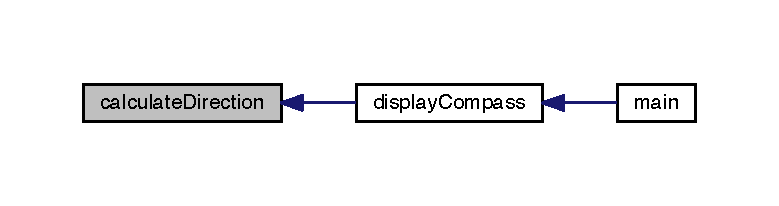
\includegraphics[width=350pt]{oled_8c_a19a885889027396a1a4db307f79458a7_icgraph}
\end{center}
\end{figure}


\index{oled.\+c@{oled.\+c}!display\+Message@{display\+Message}}
\index{display\+Message@{display\+Message}!oled.\+c@{oled.\+c}}
\subsubsection[{\texorpdfstring{display\+Message(char $\ast$string)}{displayMessage(char *string)}}]{\setlength{\rightskip}{0pt plus 5cm}void display\+Message (
\begin{DoxyParamCaption}
\item[{char $\ast$}]{string}
\end{DoxyParamCaption}
)}\hypertarget{oled_8c_a5297de8aa93b2aa08db30eb7f2ccfa21}{}\label{oled_8c_a5297de8aa93b2aa08db30eb7f2ccfa21}


Display a string in the center of the screen. 


\begin{DoxyParams}{Parameters}
{\em string} & The string to display \\
\hline
\end{DoxyParams}


Here is the call graph for this function\+:\nopagebreak
\begin{figure}[H]
\begin{center}
\leavevmode
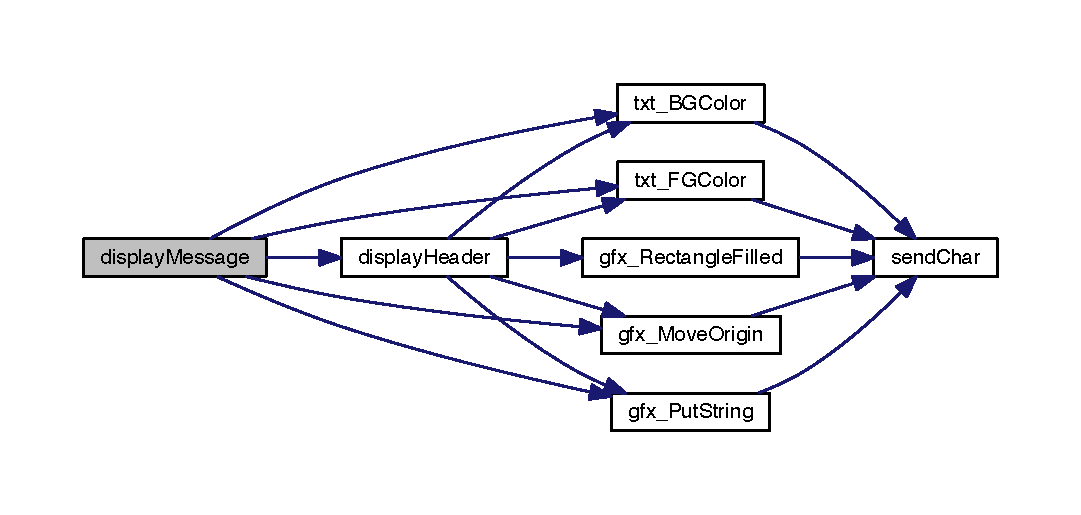
\includegraphics[width=350pt]{oled_8c_a5297de8aa93b2aa08db30eb7f2ccfa21_cgraph}
\end{center}
\end{figure}




Here is the caller graph for this function\+:\nopagebreak
\begin{figure}[H]
\begin{center}
\leavevmode
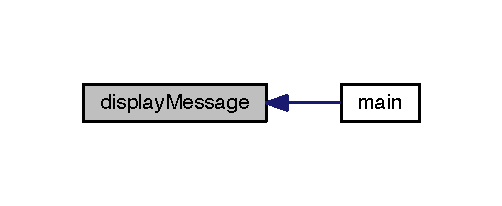
\includegraphics[width=241pt]{oled_8c_a5297de8aa93b2aa08db30eb7f2ccfa21_icgraph}
\end{center}
\end{figure}


\index{oled.\+c@{oled.\+c}!ftoa@{ftoa}}
\index{ftoa@{ftoa}!oled.\+c@{oled.\+c}}
\subsubsection[{\texorpdfstring{ftoa(char $\ast$p, float x)}{ftoa(char *p, float x)}}]{\setlength{\rightskip}{0pt plus 5cm}void ftoa (
\begin{DoxyParamCaption}
\item[{char $\ast$}]{p, }
\item[{float}]{x}
\end{DoxyParamCaption}
)}\hypertarget{oled_8c_a0c5ac5a7ba15de219c5fee85d039f971}{}\label{oled_8c_a0c5ac5a7ba15de219c5fee85d039f971}


Float to string conversion. 


\begin{DoxyParams}[1]{Parameters}
 & {\em p} & The buffer (string) \\
\hline
\mbox{\tt in}  & {\em x} & The float \\
\hline
\end{DoxyParams}


Here is the caller graph for this function\+:\nopagebreak
\begin{figure}[H]
\begin{center}
\leavevmode
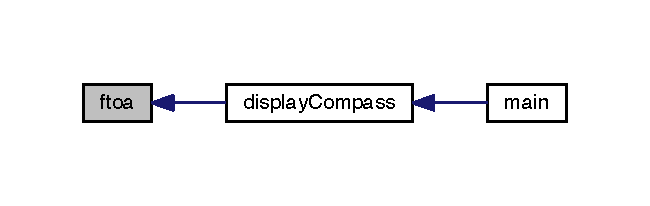
\includegraphics[width=312pt]{oled_8c_a0c5ac5a7ba15de219c5fee85d039f971_icgraph}
\end{center}
\end{figure}


\index{oled.\+c@{oled.\+c}!gfx\+\_\+\+B\+Gcolour@{gfx\+\_\+\+B\+Gcolour}}
\index{gfx\+\_\+\+B\+Gcolour@{gfx\+\_\+\+B\+Gcolour}!oled.\+c@{oled.\+c}}
\subsubsection[{\texorpdfstring{gfx\+\_\+\+B\+Gcolour(int color)}{gfx_BGcolour(int color)}}]{\setlength{\rightskip}{0pt plus 5cm}void gfx\+\_\+\+B\+Gcolour (
\begin{DoxyParamCaption}
\item[{int}]{color}
\end{DoxyParamCaption}
)}\hypertarget{oled_8c_a683fe37084d4bf81ec41bb048bb2d82d}{}\label{oled_8c_a683fe37084d4bf81ec41bb048bb2d82d}


Set the background color. 


\begin{DoxyParams}[1]{Parameters}
\mbox{\tt in}  & {\em color} & The color \\
\hline
\end{DoxyParams}


Here is the call graph for this function\+:\nopagebreak
\begin{figure}[H]
\begin{center}
\leavevmode
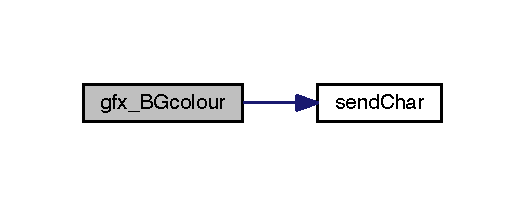
\includegraphics[width=252pt]{oled_8c_a683fe37084d4bf81ec41bb048bb2d82d_cgraph}
\end{center}
\end{figure}




Here is the caller graph for this function\+:\nopagebreak
\begin{figure}[H]
\begin{center}
\leavevmode
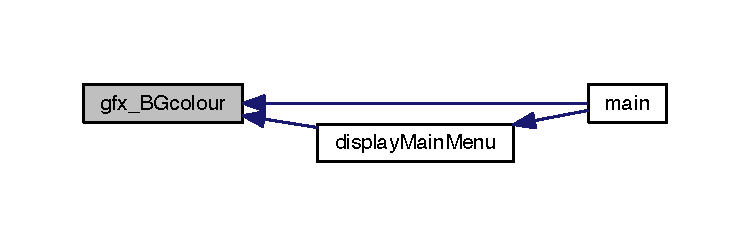
\includegraphics[width=350pt]{oled_8c_a683fe37084d4bf81ec41bb048bb2d82d_icgraph}
\end{center}
\end{figure}


\index{oled.\+c@{oled.\+c}!gfx\+\_\+\+Calculate\+Orbit@{gfx\+\_\+\+Calculate\+Orbit}}
\index{gfx\+\_\+\+Calculate\+Orbit@{gfx\+\_\+\+Calculate\+Orbit}!oled.\+c@{oled.\+c}}
\subsubsection[{\texorpdfstring{gfx\+\_\+\+Calculate\+Orbit(int angle, int distance, int $\ast$x, int $\ast$y)}{gfx_CalculateOrbit(int angle, int distance, int *x, int *y)}}]{\setlength{\rightskip}{0pt plus 5cm}void gfx\+\_\+\+Calculate\+Orbit (
\begin{DoxyParamCaption}
\item[{int}]{angle, }
\item[{int}]{distance, }
\item[{int $\ast$}]{x, }
\item[{int $\ast$}]{y}
\end{DoxyParamCaption}
)}\hypertarget{oled_8c_a51a164549510400e0dc556006c4c3b93}{}\label{oled_8c_a51a164549510400e0dc556006c4c3b93}


Calculate the (x,y) pos (orbit) from angle and distance. 


\begin{DoxyParams}[1]{Parameters}
\mbox{\tt in}  & {\em angle} & The angle \\
\hline
\mbox{\tt in}  & {\em distance} & The distance \\
\hline
 & {\em x} & The x pos computed \\
\hline
 & {\em y} & The y pos computed \\
\hline
\end{DoxyParams}


Here is the call graph for this function\+:\nopagebreak
\begin{figure}[H]
\begin{center}
\leavevmode
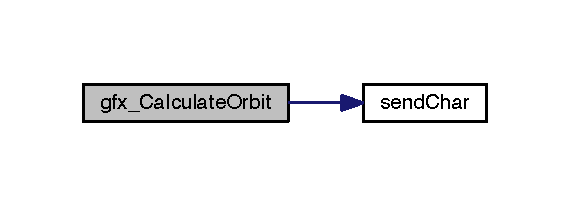
\includegraphics[width=274pt]{oled_8c_a51a164549510400e0dc556006c4c3b93_cgraph}
\end{center}
\end{figure}




Here is the caller graph for this function\+:\nopagebreak
\begin{figure}[H]
\begin{center}
\leavevmode
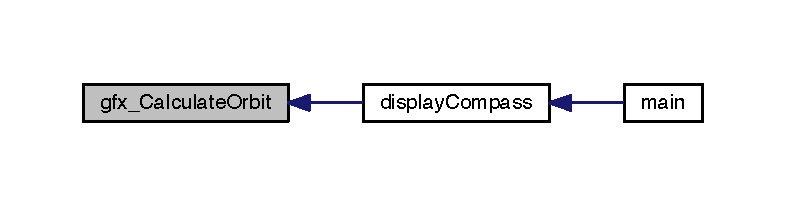
\includegraphics[width=350pt]{oled_8c_a51a164549510400e0dc556006c4c3b93_icgraph}
\end{center}
\end{figure}


\index{oled.\+c@{oled.\+c}!gfx\+\_\+\+Draw\+Circle@{gfx\+\_\+\+Draw\+Circle}}
\index{gfx\+\_\+\+Draw\+Circle@{gfx\+\_\+\+Draw\+Circle}!oled.\+c@{oled.\+c}}
\subsubsection[{\texorpdfstring{gfx\+\_\+\+Draw\+Circle(int x, int y, int radius, int color)}{gfx_DrawCircle(int x, int y, int radius, int color)}}]{\setlength{\rightskip}{0pt plus 5cm}void gfx\+\_\+\+Draw\+Circle (
\begin{DoxyParamCaption}
\item[{int}]{x, }
\item[{int}]{y, }
\item[{int}]{radius, }
\item[{int}]{color}
\end{DoxyParamCaption}
)}\hypertarget{oled_8c_ab413c7645cf3692382fd74dadedb2235}{}\label{oled_8c_ab413c7645cf3692382fd74dadedb2235}


Draw a circle. 


\begin{DoxyParams}[1]{Parameters}
\mbox{\tt in}  & {\em x} & x pos of center of the circle \\
\hline
\mbox{\tt in}  & {\em y} & y pos of center of the circle \\
\hline
\mbox{\tt in}  & {\em radius} & The radius \\
\hline
\mbox{\tt in}  & {\em color} & The color \\
\hline
\end{DoxyParams}


Here is the call graph for this function\+:\nopagebreak
\begin{figure}[H]
\begin{center}
\leavevmode
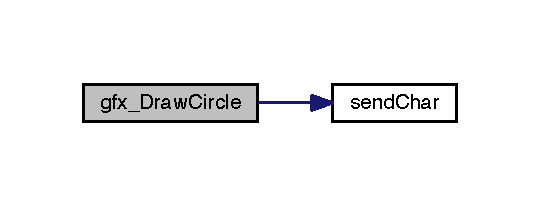
\includegraphics[width=259pt]{oled_8c_ab413c7645cf3692382fd74dadedb2235_cgraph}
\end{center}
\end{figure}




Here is the caller graph for this function\+:\nopagebreak
\begin{figure}[H]
\begin{center}
\leavevmode
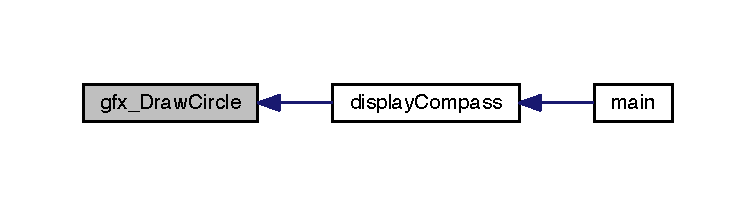
\includegraphics[width=350pt]{oled_8c_ab413c7645cf3692382fd74dadedb2235_icgraph}
\end{center}
\end{figure}


\index{oled.\+c@{oled.\+c}!gfx\+\_\+\+Draw\+Line@{gfx\+\_\+\+Draw\+Line}}
\index{gfx\+\_\+\+Draw\+Line@{gfx\+\_\+\+Draw\+Line}!oled.\+c@{oled.\+c}}
\subsubsection[{\texorpdfstring{gfx\+\_\+\+Draw\+Line(int x1, int y1, int x2, int y2, int color)}{gfx_DrawLine(int x1, int y1, int x2, int y2, int color)}}]{\setlength{\rightskip}{0pt plus 5cm}void gfx\+\_\+\+Draw\+Line (
\begin{DoxyParamCaption}
\item[{int}]{x1, }
\item[{int}]{y1, }
\item[{int}]{x2, }
\item[{int}]{y2, }
\item[{int}]{color}
\end{DoxyParamCaption}
)}\hypertarget{oled_8c_a7ba83efb69401ec85f46b0f2104f892d}{}\label{oled_8c_a7ba83efb69401ec85f46b0f2104f892d}


Draw a line. 


\begin{DoxyParams}[1]{Parameters}
\mbox{\tt in}  & {\em x1} & The x pos of the beginning of the line \\
\hline
\mbox{\tt in}  & {\em y1} & The y pos of the beginning of the line \\
\hline
\mbox{\tt in}  & {\em x2} & The x pos of the ending of the line \\
\hline
\mbox{\tt in}  & {\em y2} & The y pos of the ending of the line \\
\hline
\mbox{\tt in}  & {\em color} & The color \\
\hline
\end{DoxyParams}


Here is the call graph for this function\+:\nopagebreak
\begin{figure}[H]
\begin{center}
\leavevmode
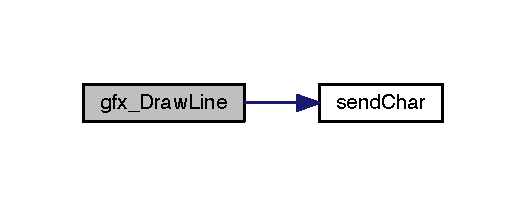
\includegraphics[width=253pt]{oled_8c_a7ba83efb69401ec85f46b0f2104f892d_cgraph}
\end{center}
\end{figure}




Here is the caller graph for this function\+:\nopagebreak
\begin{figure}[H]
\begin{center}
\leavevmode
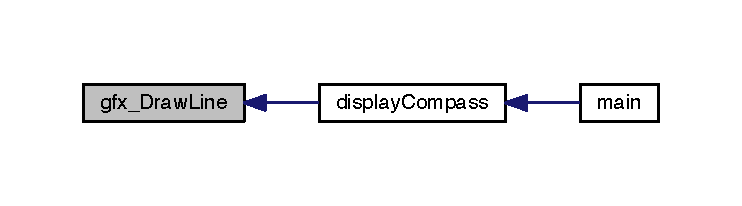
\includegraphics[width=350pt]{oled_8c_a7ba83efb69401ec85f46b0f2104f892d_icgraph}
\end{center}
\end{figure}


\index{oled.\+c@{oled.\+c}!gfx\+\_\+\+Move\+Origin@{gfx\+\_\+\+Move\+Origin}}
\index{gfx\+\_\+\+Move\+Origin@{gfx\+\_\+\+Move\+Origin}!oled.\+c@{oled.\+c}}
\subsubsection[{\texorpdfstring{gfx\+\_\+\+Move\+Origin(int x, int y)}{gfx_MoveOrigin(int x, int y)}}]{\setlength{\rightskip}{0pt plus 5cm}void gfx\+\_\+\+Move\+Origin (
\begin{DoxyParamCaption}
\item[{int}]{x, }
\item[{int}]{y}
\end{DoxyParamCaption}
)}\hypertarget{oled_8c_ac48acba04e41e0ece792c0df7baef052}{}\label{oled_8c_ac48acba04e41e0ece792c0df7baef052}


Move to origin to a position. 


\begin{DoxyParams}[1]{Parameters}
\mbox{\tt in}  & {\em x} & The new x pos \\
\hline
\mbox{\tt in}  & {\em y} & The new y pos \\
\hline
\end{DoxyParams}


Here is the call graph for this function\+:\nopagebreak
\begin{figure}[H]
\begin{center}
\leavevmode
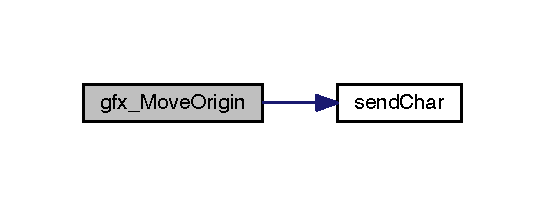
\includegraphics[width=261pt]{oled_8c_ac48acba04e41e0ece792c0df7baef052_cgraph}
\end{center}
\end{figure}




Here is the caller graph for this function\+:\nopagebreak
\begin{figure}[H]
\begin{center}
\leavevmode
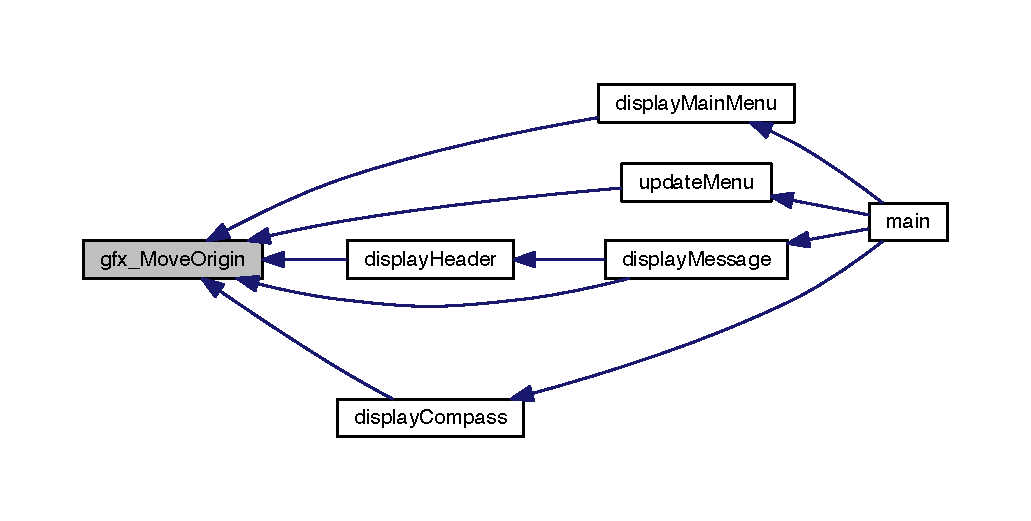
\includegraphics[width=350pt]{oled_8c_ac48acba04e41e0ece792c0df7baef052_icgraph}
\end{center}
\end{figure}


\index{oled.\+c@{oled.\+c}!gfx\+\_\+\+Put\+String@{gfx\+\_\+\+Put\+String}}
\index{gfx\+\_\+\+Put\+String@{gfx\+\_\+\+Put\+String}!oled.\+c@{oled.\+c}}
\subsubsection[{\texorpdfstring{gfx\+\_\+\+Put\+String(char $\ast$string)}{gfx_PutString(char *string)}}]{\setlength{\rightskip}{0pt plus 5cm}void gfx\+\_\+\+Put\+String (
\begin{DoxyParamCaption}
\item[{char $\ast$}]{string}
\end{DoxyParamCaption}
)}\hypertarget{oled_8c_a032ab79d797b2c886854fb9044787bf4}{}\label{oled_8c_a032ab79d797b2c886854fb9044787bf4}


Put a string on the screen. 


\begin{DoxyParams}{Parameters}
{\em string} & The string \\
\hline
\end{DoxyParams}


Here is the call graph for this function\+:\nopagebreak
\begin{figure}[H]
\begin{center}
\leavevmode
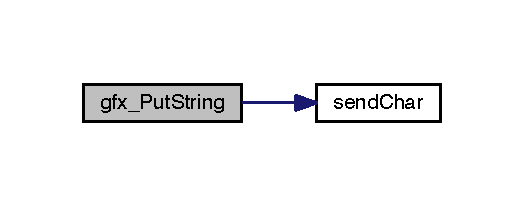
\includegraphics[width=251pt]{oled_8c_a032ab79d797b2c886854fb9044787bf4_cgraph}
\end{center}
\end{figure}




Here is the caller graph for this function\+:\nopagebreak
\begin{figure}[H]
\begin{center}
\leavevmode
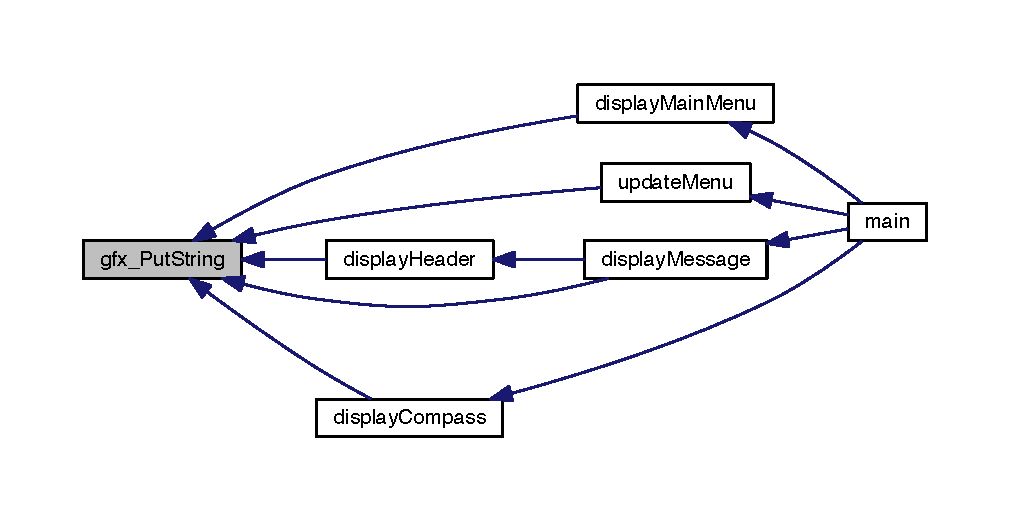
\includegraphics[width=350pt]{oled_8c_a032ab79d797b2c886854fb9044787bf4_icgraph}
\end{center}
\end{figure}


\index{oled.\+c@{oled.\+c}!gfx\+\_\+\+Rectangle@{gfx\+\_\+\+Rectangle}}
\index{gfx\+\_\+\+Rectangle@{gfx\+\_\+\+Rectangle}!oled.\+c@{oled.\+c}}
\subsubsection[{\texorpdfstring{gfx\+\_\+\+Rectangle(int x1, int y1, int x2, int y2, int color)}{gfx_Rectangle(int x1, int y1, int x2, int y2, int color)}}]{\setlength{\rightskip}{0pt plus 5cm}void gfx\+\_\+\+Rectangle (
\begin{DoxyParamCaption}
\item[{int}]{x1, }
\item[{int}]{y1, }
\item[{int}]{x2, }
\item[{int}]{y2, }
\item[{int}]{color}
\end{DoxyParamCaption}
)}\hypertarget{oled_8c_a7bf734443a53e38b4afa062783296d90}{}\label{oled_8c_a7bf734443a53e38b4afa062783296d90}


Draw a rectangle. 


\begin{DoxyParams}[1]{Parameters}
\mbox{\tt in}  & {\em x1} & The x pos of the top left corner \\
\hline
\mbox{\tt in}  & {\em y1} & The y pos of the top left corner \\
\hline
\mbox{\tt in}  & {\em x2} & The x pos of the bottom right corner \\
\hline
\mbox{\tt in}  & {\em y2} & The y pos of the bottom right corner \\
\hline
\mbox{\tt in}  & {\em color} & The color \\
\hline
\end{DoxyParams}


Here is the call graph for this function\+:\nopagebreak
\begin{figure}[H]
\begin{center}
\leavevmode
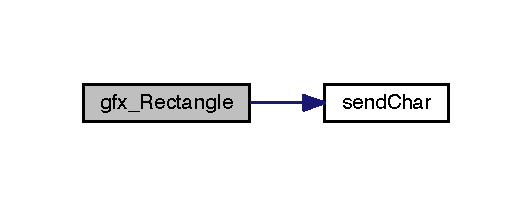
\includegraphics[width=255pt]{oled_8c_a7bf734443a53e38b4afa062783296d90_cgraph}
\end{center}
\end{figure}




Here is the caller graph for this function\+:\nopagebreak
\begin{figure}[H]
\begin{center}
\leavevmode
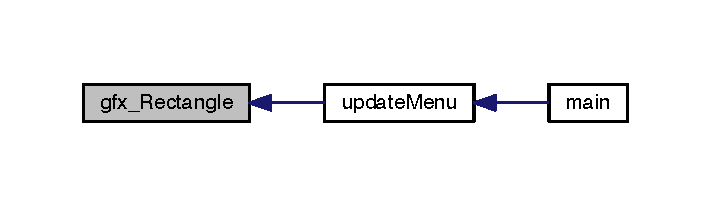
\includegraphics[width=341pt]{oled_8c_a7bf734443a53e38b4afa062783296d90_icgraph}
\end{center}
\end{figure}


\index{oled.\+c@{oled.\+c}!gfx\+\_\+\+Rectangle\+Filled@{gfx\+\_\+\+Rectangle\+Filled}}
\index{gfx\+\_\+\+Rectangle\+Filled@{gfx\+\_\+\+Rectangle\+Filled}!oled.\+c@{oled.\+c}}
\subsubsection[{\texorpdfstring{gfx\+\_\+\+Rectangle\+Filled(int x1, int y1, int x2, int y2, int color)}{gfx_RectangleFilled(int x1, int y1, int x2, int y2, int color)}}]{\setlength{\rightskip}{0pt plus 5cm}void gfx\+\_\+\+Rectangle\+Filled (
\begin{DoxyParamCaption}
\item[{int}]{x1, }
\item[{int}]{y1, }
\item[{int}]{x2, }
\item[{int}]{y2, }
\item[{int}]{color}
\end{DoxyParamCaption}
)}\hypertarget{oled_8c_a9ba037ec2bdfd47757f59d44979d6112}{}\label{oled_8c_a9ba037ec2bdfd47757f59d44979d6112}


Draw a rectangle filled with a color. 


\begin{DoxyParams}[1]{Parameters}
\mbox{\tt in}  & {\em x1} & The x pos of the top left corner \\
\hline
\mbox{\tt in}  & {\em y1} & The y pos of the top left corner \\
\hline
\mbox{\tt in}  & {\em x2} & The x pos of the bottom right corner \\
\hline
\mbox{\tt in}  & {\em y2} & The y pos of the bottom right corner \\
\hline
\mbox{\tt in}  & {\em color} & The color \\
\hline
\end{DoxyParams}


Here is the call graph for this function\+:\nopagebreak
\begin{figure}[H]
\begin{center}
\leavevmode
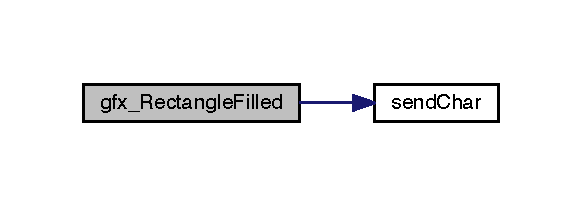
\includegraphics[width=279pt]{oled_8c_a9ba037ec2bdfd47757f59d44979d6112_cgraph}
\end{center}
\end{figure}




Here is the caller graph for this function\+:\nopagebreak
\begin{figure}[H]
\begin{center}
\leavevmode
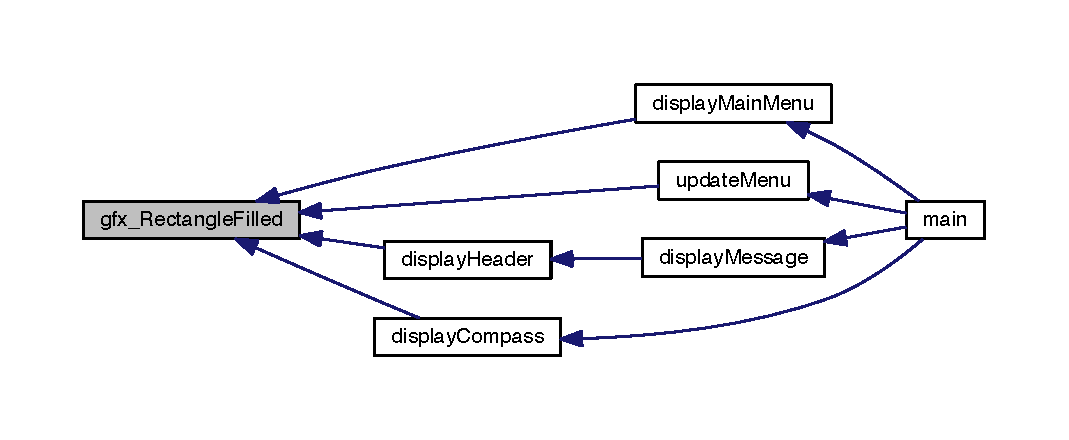
\includegraphics[width=350pt]{oled_8c_a9ba037ec2bdfd47757f59d44979d6112_icgraph}
\end{center}
\end{figure}


\index{oled.\+c@{oled.\+c}!gfx\+\_\+\+Screen\+Mode@{gfx\+\_\+\+Screen\+Mode}}
\index{gfx\+\_\+\+Screen\+Mode@{gfx\+\_\+\+Screen\+Mode}!oled.\+c@{oled.\+c}}
\subsubsection[{\texorpdfstring{gfx\+\_\+\+Screen\+Mode(int mode)}{gfx_ScreenMode(int mode)}}]{\setlength{\rightskip}{0pt plus 5cm}void gfx\+\_\+\+Screen\+Mode (
\begin{DoxyParamCaption}
\item[{int}]{mode}
\end{DoxyParamCaption}
)}\hypertarget{oled_8c_a28c8c6d46aaa97ad945248a983f2f7d0}{}\label{oled_8c_a28c8c6d46aaa97ad945248a983f2f7d0}


Screen mode (portrait/landscape) 


\begin{DoxyParams}[1]{Parameters}
\mbox{\tt in}  & {\em mode} & The mode \\
\hline
\end{DoxyParams}


Here is the call graph for this function\+:\nopagebreak
\begin{figure}[H]
\begin{center}
\leavevmode
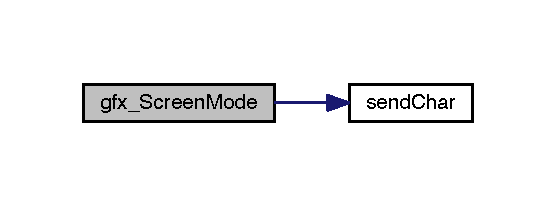
\includegraphics[width=267pt]{oled_8c_a28c8c6d46aaa97ad945248a983f2f7d0_cgraph}
\end{center}
\end{figure}




Here is the caller graph for this function\+:\nopagebreak
\begin{figure}[H]
\begin{center}
\leavevmode
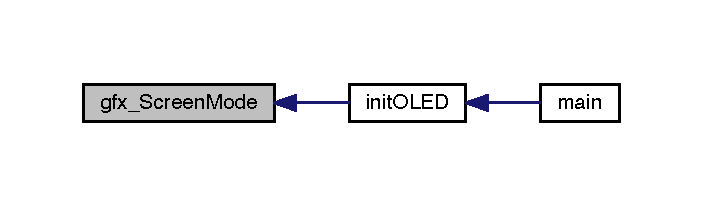
\includegraphics[width=337pt]{oled_8c_a28c8c6d46aaa97ad945248a983f2f7d0_icgraph}
\end{center}
\end{figure}


\index{oled.\+c@{oled.\+c}!send\+Char@{send\+Char}}
\index{send\+Char@{send\+Char}!oled.\+c@{oled.\+c}}
\subsubsection[{\texorpdfstring{send\+Char(int c)}{sendChar(int c)}}]{\setlength{\rightskip}{0pt plus 5cm}void send\+Char (
\begin{DoxyParamCaption}
\item[{int}]{c}
\end{DoxyParamCaption}
)}\hypertarget{oled_8c_a34fe4d307e88a437023d37e3d2f39526}{}\label{oled_8c_a34fe4d307e88a437023d37e3d2f39526}


Send char. 


\begin{DoxyParams}{Parameters}
{\em c} & The int to send \\
\hline
\end{DoxyParams}


Here is the caller graph for this function\+:\nopagebreak
\begin{figure}[H]
\begin{center}
\leavevmode
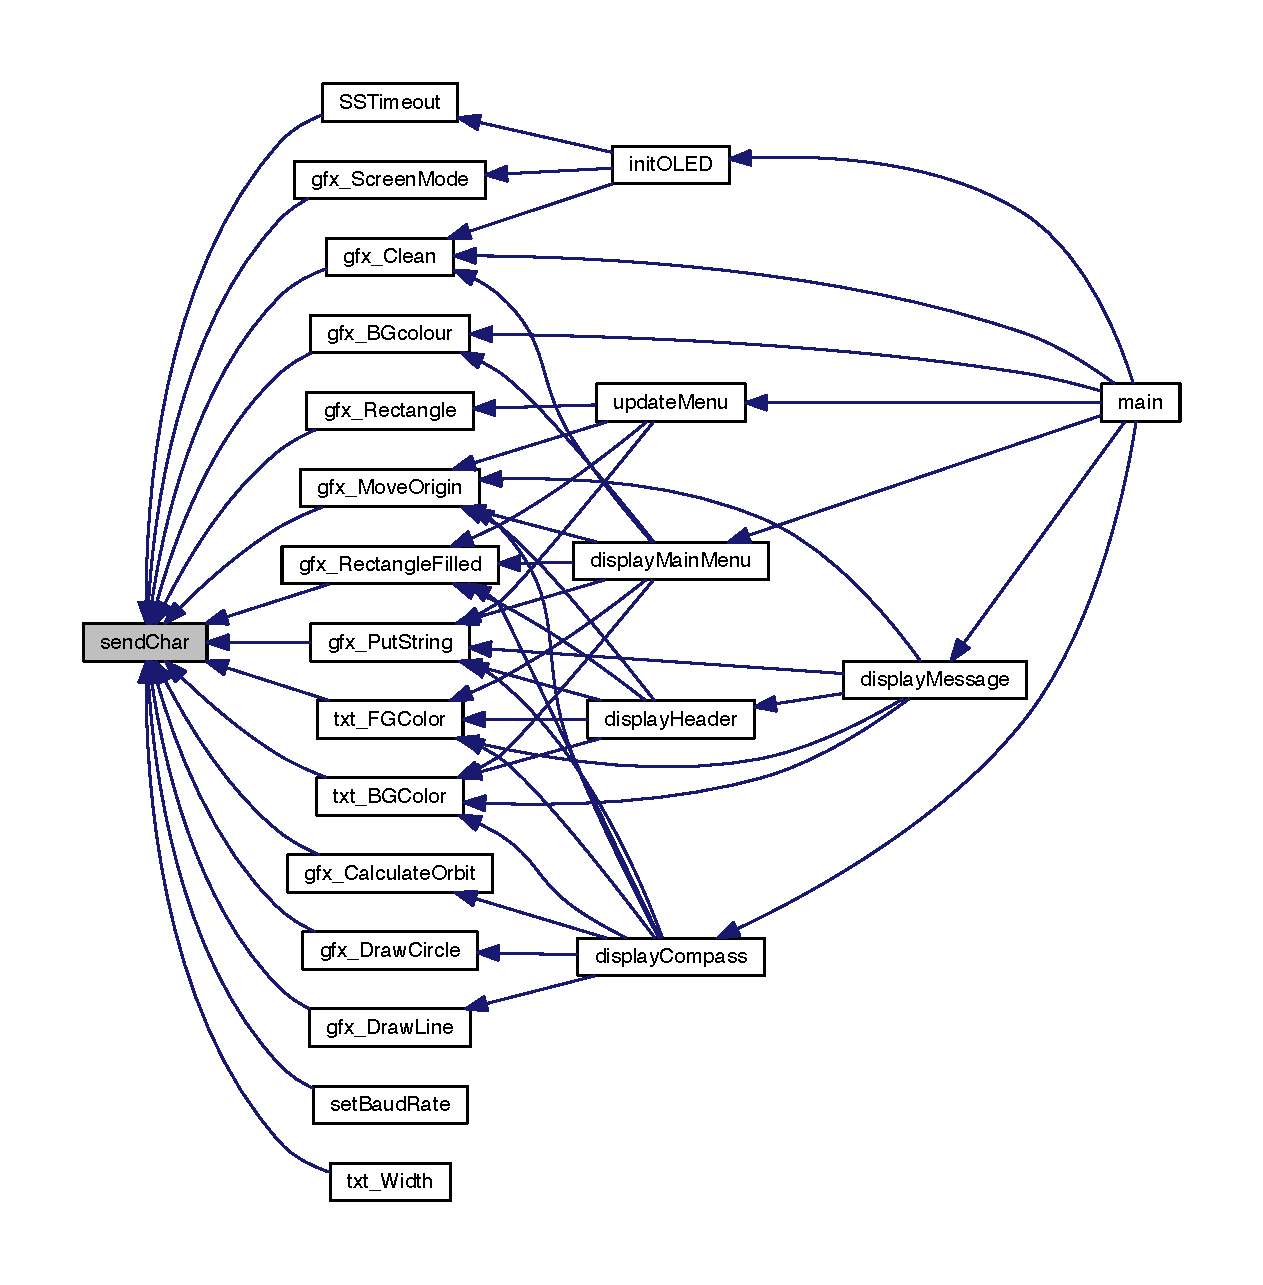
\includegraphics[width=350pt]{oled_8c_a34fe4d307e88a437023d37e3d2f39526_icgraph}
\end{center}
\end{figure}


\index{oled.\+c@{oled.\+c}!S\+S\+Timeout@{S\+S\+Timeout}}
\index{S\+S\+Timeout@{S\+S\+Timeout}!oled.\+c@{oled.\+c}}
\subsubsection[{\texorpdfstring{S\+S\+Timeout(int t)}{SSTimeout(int t)}}]{\setlength{\rightskip}{0pt plus 5cm}void S\+S\+Timeout (
\begin{DoxyParamCaption}
\item[{int}]{t}
\end{DoxyParamCaption}
)}\hypertarget{oled_8c_ac7997c7454ff66e4662893fa8bc03512}{}\label{oled_8c_ac7997c7454ff66e4662893fa8bc03512}


Screensave mode. 


\begin{DoxyParams}[1]{Parameters}
\mbox{\tt in}  & {\em t} & The mode \\
\hline
\end{DoxyParams}


Here is the call graph for this function\+:\nopagebreak
\begin{figure}[H]
\begin{center}
\leavevmode
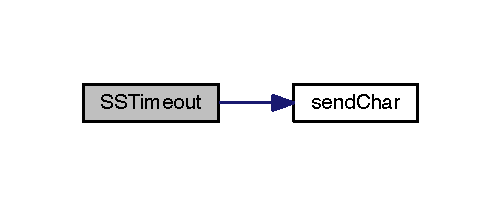
\includegraphics[width=240pt]{oled_8c_ac7997c7454ff66e4662893fa8bc03512_cgraph}
\end{center}
\end{figure}




Here is the caller graph for this function\+:\nopagebreak
\begin{figure}[H]
\begin{center}
\leavevmode
\includegraphics[width=311pt]{oled_8c_ac7997c7454ff66e4662893fa8bc03512_icgraph}
\end{center}
\end{figure}


\index{oled.\+c@{oled.\+c}!toggle\+O\+L\+E\+D\+Interrupt@{toggle\+O\+L\+E\+D\+Interrupt}}
\index{toggle\+O\+L\+E\+D\+Interrupt@{toggle\+O\+L\+E\+D\+Interrupt}!oled.\+c@{oled.\+c}}
\subsubsection[{\texorpdfstring{toggle\+O\+L\+E\+D\+Interrupt(unsigned int state)}{toggleOLEDInterrupt(unsigned int state)}}]{\setlength{\rightskip}{0pt plus 5cm}void toggle\+O\+L\+E\+D\+Interrupt (
\begin{DoxyParamCaption}
\item[{unsigned int}]{state}
\end{DoxyParamCaption}
)}\hypertarget{oled_8c_a458006637c584f6db260748e25615708}{}\label{oled_8c_a458006637c584f6db260748e25615708}


Toggle O\+L\+ED interrupt. 

1 = interrupt enable for O\+L\+ED, 0 = disable


\begin{DoxyParams}{Parameters}
{\em state} & The new state \\
\hline
\end{DoxyParams}


Here is the caller graph for this function\+:\nopagebreak
\begin{figure}[H]
\begin{center}
\leavevmode
\includegraphics[width=350pt]{oled_8c_a458006637c584f6db260748e25615708_icgraph}
\end{center}
\end{figure}


\index{oled.\+c@{oled.\+c}!txt\+\_\+\+B\+G\+Color@{txt\+\_\+\+B\+G\+Color}}
\index{txt\+\_\+\+B\+G\+Color@{txt\+\_\+\+B\+G\+Color}!oled.\+c@{oled.\+c}}
\subsubsection[{\texorpdfstring{txt\+\_\+\+B\+G\+Color(int color)}{txt_BGColor(int color)}}]{\setlength{\rightskip}{0pt plus 5cm}void txt\+\_\+\+B\+G\+Color (
\begin{DoxyParamCaption}
\item[{int}]{color}
\end{DoxyParamCaption}
)}\hypertarget{oled_8c_ad673132fcf81110f70f687c441d2c218}{}\label{oled_8c_ad673132fcf81110f70f687c441d2c218}


Set the text background color. 


\begin{DoxyParams}[1]{Parameters}
\mbox{\tt in}  & {\em color} & The color \\
\hline
\end{DoxyParams}


Here is the call graph for this function\+:\nopagebreak
\begin{figure}[H]
\begin{center}
\leavevmode
\includegraphics[width=246pt]{oled_8c_ad673132fcf81110f70f687c441d2c218_cgraph}
\end{center}
\end{figure}




Here is the caller graph for this function\+:\nopagebreak
\begin{figure}[H]
\begin{center}
\leavevmode
\includegraphics[width=350pt]{oled_8c_ad673132fcf81110f70f687c441d2c218_icgraph}
\end{center}
\end{figure}


\index{oled.\+c@{oled.\+c}!txt\+\_\+\+F\+G\+Color@{txt\+\_\+\+F\+G\+Color}}
\index{txt\+\_\+\+F\+G\+Color@{txt\+\_\+\+F\+G\+Color}!oled.\+c@{oled.\+c}}
\subsubsection[{\texorpdfstring{txt\+\_\+\+F\+G\+Color(int color)}{txt_FGColor(int color)}}]{\setlength{\rightskip}{0pt plus 5cm}void txt\+\_\+\+F\+G\+Color (
\begin{DoxyParamCaption}
\item[{int}]{color}
\end{DoxyParamCaption}
)}\hypertarget{oled_8c_a1ad10b8c9c7f57a38615788ef00adbfd}{}\label{oled_8c_a1ad10b8c9c7f57a38615788ef00adbfd}


Set the text color. 


\begin{DoxyParams}[1]{Parameters}
\mbox{\tt in}  & {\em color} & The color \\
\hline
\end{DoxyParams}


Here is the call graph for this function\+:\nopagebreak
\begin{figure}[H]
\begin{center}
\leavevmode
\includegraphics[width=245pt]{oled_8c_a1ad10b8c9c7f57a38615788ef00adbfd_cgraph}
\end{center}
\end{figure}




Here is the caller graph for this function\+:\nopagebreak
\begin{figure}[H]
\begin{center}
\leavevmode
\includegraphics[width=350pt]{oled_8c_a1ad10b8c9c7f57a38615788ef00adbfd_icgraph}
\end{center}
\end{figure}


\index{oled.\+c@{oled.\+c}!txt\+\_\+\+Width@{txt\+\_\+\+Width}}
\index{txt\+\_\+\+Width@{txt\+\_\+\+Width}!oled.\+c@{oled.\+c}}
\subsubsection[{\texorpdfstring{txt\+\_\+\+Width(int multi)}{txt_Width(int multi)}}]{\setlength{\rightskip}{0pt plus 5cm}void txt\+\_\+\+Width (
\begin{DoxyParamCaption}
\item[{int}]{multi}
\end{DoxyParamCaption}
)}\hypertarget{oled_8c_a9f77c9a0e006b4b9798d3ddc93e5c020}{}\label{oled_8c_a9f77c9a0e006b4b9798d3ddc93e5c020}


Set the width of the text. 


\begin{DoxyParams}[1]{Parameters}
\mbox{\tt in}  & {\em multi} & The multi \\
\hline
\end{DoxyParams}


Here is the call graph for this function\+:\nopagebreak
\begin{figure}[H]
\begin{center}
\leavevmode
\includegraphics[width=233pt]{oled_8c_a9f77c9a0e006b4b9798d3ddc93e5c020_cgraph}
\end{center}
\end{figure}




\subsection{Variable Documentation}
\index{oled.\+c@{oled.\+c}!display\+Has\+Been\+Updated@{display\+Has\+Been\+Updated}}
\index{display\+Has\+Been\+Updated@{display\+Has\+Been\+Updated}!oled.\+c@{oled.\+c}}
\subsubsection[{\texorpdfstring{display\+Has\+Been\+Updated}{displayHasBeenUpdated}}]{\setlength{\rightskip}{0pt plus 5cm}int display\+Has\+Been\+Updated}\hypertarget{oled_8c_a3aaa091434c6f423bf9f2ea6bd0f1637}{}\label{oled_8c_a3aaa091434c6f423bf9f2ea6bd0f1637}
Is the display has been updated, aka needed \index{oled.\+c@{oled.\+c}!mode\+Display@{mode\+Display}}
\index{mode\+Display@{mode\+Display}!oled.\+c@{oled.\+c}}
\subsubsection[{\texorpdfstring{mode\+Display}{modeDisplay}}]{\setlength{\rightskip}{0pt plus 5cm}unsigned int mode\+Display = {\bf M\+D\+\_\+\+S\+H\+U\+T\+D\+O\+WN}}\hypertarget{oled_8c_ab689e5e58122785f3fb3145de9489b5a}{}\label{oled_8c_ab689e5e58122785f3fb3145de9489b5a}
What mode is selected right now \index{oled.\+c@{oled.\+c}!old\+Mode\+Display@{old\+Mode\+Display}}
\index{old\+Mode\+Display@{old\+Mode\+Display}!oled.\+c@{oled.\+c}}
\subsubsection[{\texorpdfstring{old\+Mode\+Display}{oldModeDisplay}}]{\setlength{\rightskip}{0pt plus 5cm}unsigned int old\+Mode\+Display}\hypertarget{oled_8c_aa7651e004151fc14802a52f62a381bd5}{}\label{oled_8c_aa7651e004151fc14802a52f62a381bd5}
What mode was selected just before 
\hypertarget{oled_8h}{}\section{oled.\+h File Reference}
\label{oled_8h}\index{oled.\+h@{oled.\+h}}


File containing the O\+L\+ED functions.  


This graph shows which files directly or indirectly include this file\+:\nopagebreak
\begin{figure}[H]
\begin{center}
\leavevmode
\includegraphics[width=303pt]{oled_8h__dep__incl}
\end{center}
\end{figure}
\subsection*{Macros}
\begin{DoxyCompactItemize}
\item 
\#define \hyperlink{oled_8h_a1f957b762e025dae67967a36c86dcfc1}{C\+U\+R\+R\+E\+NT}~1\hypertarget{oled_8h_a1f957b762e025dae67967a36c86dcfc1}{}\label{oled_8h_a1f957b762e025dae67967a36c86dcfc1}

\begin{DoxyCompactList}\small\item\em Current. \end{DoxyCompactList}\item 
\#define \hyperlink{oled_8h_a15484b7c03434f6dbd2016eaefd0df9f}{O\+LD}~0\hypertarget{oled_8h_a15484b7c03434f6dbd2016eaefd0df9f}{}\label{oled_8h_a15484b7c03434f6dbd2016eaefd0df9f}

\begin{DoxyCompactList}\small\item\em O\+LD. \end{DoxyCompactList}\item 
\#define \hyperlink{oled_8h_a553b74b4ed069b4ce3393d50d9fdf76f}{M\+D\+\_\+\+C\+O\+M\+P\+A\+SS}~0\hypertarget{oled_8h_a553b74b4ed069b4ce3393d50d9fdf76f}{}\label{oled_8h_a553b74b4ed069b4ce3393d50d9fdf76f}

\begin{DoxyCompactList}\small\item\em Mode selected on display is compass. \end{DoxyCompactList}\item 
\#define \hyperlink{oled_8h_a8aae6da3e973f81045e829bb6512f51b}{M\+D\+\_\+\+N\+A\+V\+IG}~1\hypertarget{oled_8h_a8aae6da3e973f81045e829bb6512f51b}{}\label{oled_8h_a8aae6da3e973f81045e829bb6512f51b}

\begin{DoxyCompactList}\small\item\em Mode selected on display is naviguation. \end{DoxyCompactList}\item 
\#define \hyperlink{oled_8h_ad0e26341e7b7fc71000c7c7331e4f821}{M\+D\+\_\+\+R\+E\+C\+O\+RD}~2\hypertarget{oled_8h_ad0e26341e7b7fc71000c7c7331e4f821}{}\label{oled_8h_ad0e26341e7b7fc71000c7c7331e4f821}

\begin{DoxyCompactList}\small\item\em Mode selected on display is record. \end{DoxyCompactList}\item 
\#define \hyperlink{oled_8h_afe81a2875c64634e4f3b9dcc0aed2001}{M\+D\+\_\+\+S\+H\+U\+T\+D\+O\+WN}~3\hypertarget{oled_8h_afe81a2875c64634e4f3b9dcc0aed2001}{}\label{oled_8h_afe81a2875c64634e4f3b9dcc0aed2001}

\begin{DoxyCompactList}\small\item\em Mode selected on display is shutdown. \end{DoxyCompactList}\item 
\#define \hyperlink{oled_8h_a655c84af1b0034986ff56e12e84f983d}{N\+O\+NE}~\char`\"{}\char`\"{}\hypertarget{oled_8h_a655c84af1b0034986ff56e12e84f983d}{}\label{oled_8h_a655c84af1b0034986ff56e12e84f983d}

\begin{DoxyCompactList}\small\item\em Direction is none. \end{DoxyCompactList}\item 
\#define \hyperlink{oled_8h_a1711232abf72723b5216c206e6bbb175}{N\+O\+R\+TH}~\char`\"{}N\char`\"{}\hypertarget{oled_8h_a1711232abf72723b5216c206e6bbb175}{}\label{oled_8h_a1711232abf72723b5216c206e6bbb175}

\begin{DoxyCompactList}\small\item\em Direction is north. \end{DoxyCompactList}\item 
\#define \hyperlink{oled_8h_a5af9139e882aef6c820ae908589a40d6}{NE}~\char`\"{}NE\char`\"{}\hypertarget{oled_8h_a5af9139e882aef6c820ae908589a40d6}{}\label{oled_8h_a5af9139e882aef6c820ae908589a40d6}

\begin{DoxyCompactList}\small\item\em Direction is north-\/east. \end{DoxyCompactList}\item 
\#define \hyperlink{oled_8h_a072a1ef1143314441742097b799be322}{E\+A\+ST}~\char`\"{}E\char`\"{}\hypertarget{oled_8h_a072a1ef1143314441742097b799be322}{}\label{oled_8h_a072a1ef1143314441742097b799be322}

\begin{DoxyCompactList}\small\item\em Direction is east. \end{DoxyCompactList}\item 
\#define \hyperlink{oled_8h_a18bbe716f5be6adbd2150139244c0262}{SE}~\char`\"{}SE\char`\"{}\hypertarget{oled_8h_a18bbe716f5be6adbd2150139244c0262}{}\label{oled_8h_a18bbe716f5be6adbd2150139244c0262}

\begin{DoxyCompactList}\small\item\em Direction is south-\/east. \end{DoxyCompactList}\item 
\#define \hyperlink{oled_8h_af3830320fe6287f717dca9669f417950}{S\+O\+U\+TH}~\char`\"{}S\char`\"{}\hypertarget{oled_8h_af3830320fe6287f717dca9669f417950}{}\label{oled_8h_af3830320fe6287f717dca9669f417950}

\begin{DoxyCompactList}\small\item\em Direction is south. \end{DoxyCompactList}\item 
\#define \hyperlink{oled_8h_a4b95e941f44a20ea60512bbe2065f0b6}{SW}~\char`\"{}SO\char`\"{}\hypertarget{oled_8h_a4b95e941f44a20ea60512bbe2065f0b6}{}\label{oled_8h_a4b95e941f44a20ea60512bbe2065f0b6}

\begin{DoxyCompactList}\small\item\em Direction is south-\/west. \end{DoxyCompactList}\item 
\#define \hyperlink{oled_8h_a755da365a2f771fdb9e15af22fee7d74}{W\+E\+ST}~\char`\"{}O\char`\"{}\hypertarget{oled_8h_a755da365a2f771fdb9e15af22fee7d74}{}\label{oled_8h_a755da365a2f771fdb9e15af22fee7d74}

\begin{DoxyCompactList}\small\item\em Direction is west. \end{DoxyCompactList}\item 
\#define \hyperlink{oled_8h_af9cccf331f045b89a9f12366df5f7687}{NW}~\char`\"{}NO\char`\"{}\hypertarget{oled_8h_af9cccf331f045b89a9f12366df5f7687}{}\label{oled_8h_af9cccf331f045b89a9f12366df5f7687}

\begin{DoxyCompactList}\small\item\em Direction is north-\/west. \end{DoxyCompactList}\item 
\#define \hyperlink{oled_8h_ab8eb2e510170a882284d58a254a8153c}{O\+L\+E\+D\+\_\+\+A\+N\+S\+W\+E\+R\+\_\+\+A\+CK}~6\hypertarget{oled_8h_ab8eb2e510170a882284d58a254a8153c}{}\label{oled_8h_ab8eb2e510170a882284d58a254a8153c}

\begin{DoxyCompactList}\small\item\em O\+L\+ED respond is A\+CK. \end{DoxyCompactList}\item 
\#define \hyperlink{oled_8h_a2daac8ef505617938fc493bbc7b0d803}{A\+L\+I\+C\+E\+B\+L\+UE}~0x\+F7\+DF\hypertarget{oled_8h_a2daac8ef505617938fc493bbc7b0d803}{}\label{oled_8h_a2daac8ef505617938fc493bbc7b0d803}

\begin{DoxyCompactList}\small\item\em Color. \end{DoxyCompactList}\item 
\#define \hyperlink{oled_8h_aa248d50884a3fb64150f04dfb9a4a3b2}{A\+N\+T\+I\+Q\+U\+E\+W\+H\+I\+TE}~0x\+F\+F5A\hypertarget{oled_8h_aa248d50884a3fb64150f04dfb9a4a3b2}{}\label{oled_8h_aa248d50884a3fb64150f04dfb9a4a3b2}

\begin{DoxyCompactList}\small\item\em Color. \end{DoxyCompactList}\item 
\#define \hyperlink{oled_8h_a03f3dfd90aa5fafc6c690f215b489976}{A\+Q\+UA}~0x07\+FF\hypertarget{oled_8h_a03f3dfd90aa5fafc6c690f215b489976}{}\label{oled_8h_a03f3dfd90aa5fafc6c690f215b489976}

\begin{DoxyCompactList}\small\item\em Color. \end{DoxyCompactList}\item 
\#define \hyperlink{oled_8h_a135eff048f5a270f0eb1b06992983eac}{A\+Q\+U\+A\+M\+A\+R\+I\+NE}~0x7\+F\+FA\hypertarget{oled_8h_a135eff048f5a270f0eb1b06992983eac}{}\label{oled_8h_a135eff048f5a270f0eb1b06992983eac}

\begin{DoxyCompactList}\small\item\em Color. \end{DoxyCompactList}\item 
\#define \hyperlink{oled_8h_a7ece2444eec90b2c4bac5100b24bb116}{A\+Z\+U\+RE}~0x\+F7\+FF\hypertarget{oled_8h_a7ece2444eec90b2c4bac5100b24bb116}{}\label{oled_8h_a7ece2444eec90b2c4bac5100b24bb116}

\begin{DoxyCompactList}\small\item\em Color. \end{DoxyCompactList}\item 
\#define \hyperlink{oled_8h_a1ea47e8fb8d56ffc617fabdc1e3fdb69}{B\+E\+I\+GE}~0x\+F7\+BB\hypertarget{oled_8h_a1ea47e8fb8d56ffc617fabdc1e3fdb69}{}\label{oled_8h_a1ea47e8fb8d56ffc617fabdc1e3fdb69}

\begin{DoxyCompactList}\small\item\em Color. \end{DoxyCompactList}\item 
\#define \hyperlink{oled_8h_ab9be999e6209c326cff7617631ec69bc}{B\+I\+S\+Q\+UE}~0x\+F\+F38\hypertarget{oled_8h_ab9be999e6209c326cff7617631ec69bc}{}\label{oled_8h_ab9be999e6209c326cff7617631ec69bc}

\begin{DoxyCompactList}\small\item\em Color. \end{DoxyCompactList}\item 
\#define \hyperlink{oled_8h_a7b3b25cba33b07c303f3060fe41887f6}{B\+L\+A\+CK}~0x0000\hypertarget{oled_8h_a7b3b25cba33b07c303f3060fe41887f6}{}\label{oled_8h_a7b3b25cba33b07c303f3060fe41887f6}

\begin{DoxyCompactList}\small\item\em Color. \end{DoxyCompactList}\item 
\#define \hyperlink{oled_8h_ab8c6aad0e9e8a38082041d55f4f88167}{B\+L\+A\+N\+C\+H\+E\+D\+A\+L\+M\+O\+ND}~0x\+F\+F59\hypertarget{oled_8h_ab8c6aad0e9e8a38082041d55f4f88167}{}\label{oled_8h_ab8c6aad0e9e8a38082041d55f4f88167}

\begin{DoxyCompactList}\small\item\em Color. \end{DoxyCompactList}\item 
\#define \hyperlink{oled_8h_a79d10e672abb49ad63eeaa8aaef57c38}{B\+L\+UE}~0x001F\hypertarget{oled_8h_a79d10e672abb49ad63eeaa8aaef57c38}{}\label{oled_8h_a79d10e672abb49ad63eeaa8aaef57c38}

\begin{DoxyCompactList}\small\item\em Color. \end{DoxyCompactList}\item 
\#define \hyperlink{oled_8h_a96b05e7735aec315f79498f18e69db32}{B\+L\+U\+E\+V\+I\+O\+L\+ET}~0x895C\hypertarget{oled_8h_a96b05e7735aec315f79498f18e69db32}{}\label{oled_8h_a96b05e7735aec315f79498f18e69db32}

\begin{DoxyCompactList}\small\item\em Color. \end{DoxyCompactList}\item 
\#define \hyperlink{oled_8h_ab2baea56ece91306020afd6d77fd19f9}{B\+R\+O\+WN}~0x\+A145\hypertarget{oled_8h_ab2baea56ece91306020afd6d77fd19f9}{}\label{oled_8h_ab2baea56ece91306020afd6d77fd19f9}

\begin{DoxyCompactList}\small\item\em Color. \end{DoxyCompactList}\item 
\#define \hyperlink{oled_8h_a64cac34987143c9b59056d4b02911666}{B\+U\+R\+L\+Y\+W\+O\+OD}~0x\+D\+D\+D0\hypertarget{oled_8h_a64cac34987143c9b59056d4b02911666}{}\label{oled_8h_a64cac34987143c9b59056d4b02911666}

\begin{DoxyCompactList}\small\item\em Color. \end{DoxyCompactList}\item 
\#define \hyperlink{oled_8h_aa3bcc5235ae38e5e20d20999bfe74638}{C\+A\+D\+E\+T\+B\+L\+UE}~0x5\+C\+F4\hypertarget{oled_8h_aa3bcc5235ae38e5e20d20999bfe74638}{}\label{oled_8h_aa3bcc5235ae38e5e20d20999bfe74638}

\begin{DoxyCompactList}\small\item\em Color. \end{DoxyCompactList}\item 
\#define \hyperlink{oled_8h_acd3075eb752a4b0eb2925e2a85b93662}{C\+H\+A\+R\+T\+R\+E\+U\+SE}~0x7\+F\+E0\hypertarget{oled_8h_acd3075eb752a4b0eb2925e2a85b93662}{}\label{oled_8h_acd3075eb752a4b0eb2925e2a85b93662}

\begin{DoxyCompactList}\small\item\em Color. \end{DoxyCompactList}\item 
\#define \hyperlink{oled_8h_ac21ee2d76134a9a1453c3e3b1a786173}{C\+H\+O\+C\+O\+L\+A\+TE}~0x\+D343\hypertarget{oled_8h_ac21ee2d76134a9a1453c3e3b1a786173}{}\label{oled_8h_ac21ee2d76134a9a1453c3e3b1a786173}

\begin{DoxyCompactList}\small\item\em Color. \end{DoxyCompactList}\item 
\#define \hyperlink{oled_8h_a1e1791735cb7832943c0d3c58936da44}{C\+O\+R\+AL}~0x\+F\+B\+EA\hypertarget{oled_8h_a1e1791735cb7832943c0d3c58936da44}{}\label{oled_8h_a1e1791735cb7832943c0d3c58936da44}

\begin{DoxyCompactList}\small\item\em Color. \end{DoxyCompactList}\item 
\#define \hyperlink{oled_8h_a0f95c316ab2b1abf70495663ba0bc942}{C\+O\+R\+N\+F\+L\+O\+W\+E\+R\+B\+L\+UE}~0x64\+BD\hypertarget{oled_8h_a0f95c316ab2b1abf70495663ba0bc942}{}\label{oled_8h_a0f95c316ab2b1abf70495663ba0bc942}

\begin{DoxyCompactList}\small\item\em Color. \end{DoxyCompactList}\item 
\#define \hyperlink{oled_8h_a390dafeb3ff47e220f8629ee9a6bcab3}{C\+O\+R\+N\+S\+I\+LK}~0x\+F\+F\+DB\hypertarget{oled_8h_a390dafeb3ff47e220f8629ee9a6bcab3}{}\label{oled_8h_a390dafeb3ff47e220f8629ee9a6bcab3}

\begin{DoxyCompactList}\small\item\em Color. \end{DoxyCompactList}\item 
\#define \hyperlink{oled_8h_ad6a57d13073a8ef53dcb68d625fbda0b}{C\+R\+I\+M\+S\+ON}~0x\+D8\+A7\hypertarget{oled_8h_ad6a57d13073a8ef53dcb68d625fbda0b}{}\label{oled_8h_ad6a57d13073a8ef53dcb68d625fbda0b}

\begin{DoxyCompactList}\small\item\em Color. \end{DoxyCompactList}\item 
\#define \hyperlink{oled_8h_ad243f93c16bc4c1d3e0a13b84421d760}{C\+Y\+AN}~0x07\+FF\hypertarget{oled_8h_ad243f93c16bc4c1d3e0a13b84421d760}{}\label{oled_8h_ad243f93c16bc4c1d3e0a13b84421d760}

\begin{DoxyCompactList}\small\item\em Color. \end{DoxyCompactList}\item 
\#define \hyperlink{oled_8h_aa1cb63adface880613149574fc26069c}{D\+A\+R\+K\+B\+L\+UE}~0x0011\hypertarget{oled_8h_aa1cb63adface880613149574fc26069c}{}\label{oled_8h_aa1cb63adface880613149574fc26069c}

\begin{DoxyCompactList}\small\item\em Color. \end{DoxyCompactList}\item 
\#define \hyperlink{oled_8h_a15c55ca6a5cd0dc32804985d35dd7459}{D\+A\+R\+K\+C\+Y\+AN}~0x0451\hypertarget{oled_8h_a15c55ca6a5cd0dc32804985d35dd7459}{}\label{oled_8h_a15c55ca6a5cd0dc32804985d35dd7459}

\begin{DoxyCompactList}\small\item\em Color. \end{DoxyCompactList}\item 
\#define \hyperlink{oled_8h_afcc93bd1f56f475d713e5549076aff72}{D\+A\+R\+K\+G\+O\+L\+D\+E\+N\+R\+OD}~0x\+B\+C21\hypertarget{oled_8h_afcc93bd1f56f475d713e5549076aff72}{}\label{oled_8h_afcc93bd1f56f475d713e5549076aff72}

\begin{DoxyCompactList}\small\item\em Color. \end{DoxyCompactList}\item 
\#define \hyperlink{oled_8h_a4c08a6ce38e246fb2e4443329645aa5a}{D\+A\+R\+K\+G\+R\+AY}~0x\+A\+D55\hypertarget{oled_8h_a4c08a6ce38e246fb2e4443329645aa5a}{}\label{oled_8h_a4c08a6ce38e246fb2e4443329645aa5a}

\begin{DoxyCompactList}\small\item\em Color. \end{DoxyCompactList}\item 
\#define \hyperlink{oled_8h_a417b60720dd3d179e06f7efecca21123}{D\+A\+R\+K\+G\+R\+E\+EN}~0x0320\hypertarget{oled_8h_a417b60720dd3d179e06f7efecca21123}{}\label{oled_8h_a417b60720dd3d179e06f7efecca21123}

\begin{DoxyCompactList}\small\item\em Color. \end{DoxyCompactList}\item 
\#define \hyperlink{oled_8h_a6684bb4976288653d7e29dff53e54833}{D\+A\+R\+K\+K\+H\+A\+KI}~0x\+B\+D\+AD\hypertarget{oled_8h_a6684bb4976288653d7e29dff53e54833}{}\label{oled_8h_a6684bb4976288653d7e29dff53e54833}

\begin{DoxyCompactList}\small\item\em Color. \end{DoxyCompactList}\item 
\#define \hyperlink{oled_8h_aeacd625bd5c036991a3fac70a1eadfe9}{D\+A\+R\+K\+M\+A\+G\+E\+N\+TA}~0x8811\hypertarget{oled_8h_aeacd625bd5c036991a3fac70a1eadfe9}{}\label{oled_8h_aeacd625bd5c036991a3fac70a1eadfe9}

\begin{DoxyCompactList}\small\item\em Color. \end{DoxyCompactList}\item 
\#define \hyperlink{oled_8h_a04e04763f2968631784c7073321f580b}{D\+A\+R\+K\+O\+L\+I\+V\+E\+G\+R\+E\+EN}~0x5345\hypertarget{oled_8h_a04e04763f2968631784c7073321f580b}{}\label{oled_8h_a04e04763f2968631784c7073321f580b}

\begin{DoxyCompactList}\small\item\em Color. \end{DoxyCompactList}\item 
\#define \hyperlink{oled_8h_a2163a09f9745d579ac1e3e3ccbebde96}{D\+A\+R\+K\+O\+R\+A\+N\+GE}~0x\+F\+C60\hypertarget{oled_8h_a2163a09f9745d579ac1e3e3ccbebde96}{}\label{oled_8h_a2163a09f9745d579ac1e3e3ccbebde96}

\begin{DoxyCompactList}\small\item\em Color. \end{DoxyCompactList}\item 
\#define \hyperlink{oled_8h_a2124a5998ec14df2f465da29a923b621}{D\+A\+R\+K\+O\+R\+C\+H\+ID}~0x9999\hypertarget{oled_8h_a2124a5998ec14df2f465da29a923b621}{}\label{oled_8h_a2124a5998ec14df2f465da29a923b621}

\begin{DoxyCompactList}\small\item\em Color. \end{DoxyCompactList}\item 
\#define \hyperlink{oled_8h_a963a09a681f27b9562bd1ae1c7bf21ac}{D\+A\+R\+K\+R\+ED}~0x8800\hypertarget{oled_8h_a963a09a681f27b9562bd1ae1c7bf21ac}{}\label{oled_8h_a963a09a681f27b9562bd1ae1c7bf21ac}

\begin{DoxyCompactList}\small\item\em Color. \end{DoxyCompactList}\item 
\#define \hyperlink{oled_8h_a59decdba14e522c7777583438b0555b4}{D\+A\+R\+K\+S\+A\+L\+M\+ON}~0x\+E\+C\+AF\hypertarget{oled_8h_a59decdba14e522c7777583438b0555b4}{}\label{oled_8h_a59decdba14e522c7777583438b0555b4}

\begin{DoxyCompactList}\small\item\em Color. \end{DoxyCompactList}\item 
\#define \hyperlink{oled_8h_ad2543216654bf22bce30a3700b6b65a6}{D\+A\+R\+K\+S\+E\+A\+G\+R\+E\+EN}~0x8\+D\+F1\hypertarget{oled_8h_ad2543216654bf22bce30a3700b6b65a6}{}\label{oled_8h_ad2543216654bf22bce30a3700b6b65a6}

\begin{DoxyCompactList}\small\item\em Color. \end{DoxyCompactList}\item 
\#define \hyperlink{oled_8h_a667fd1de111d3ba3258abe74e628a6ea}{D\+A\+R\+K\+S\+L\+A\+T\+E\+B\+L\+UE}~0x49\+F1\hypertarget{oled_8h_a667fd1de111d3ba3258abe74e628a6ea}{}\label{oled_8h_a667fd1de111d3ba3258abe74e628a6ea}

\begin{DoxyCompactList}\small\item\em Color. \end{DoxyCompactList}\item 
\#define \hyperlink{oled_8h_ac63a9f674c5007205ae155a31840feb5}{D\+A\+R\+K\+S\+L\+A\+T\+E\+G\+R\+AY}~0x2\+A69\hypertarget{oled_8h_ac63a9f674c5007205ae155a31840feb5}{}\label{oled_8h_ac63a9f674c5007205ae155a31840feb5}

\begin{DoxyCompactList}\small\item\em Color. \end{DoxyCompactList}\item 
\#define \hyperlink{oled_8h_a79785413d86ef82283758338fd31fd55}{D\+A\+R\+K\+T\+U\+R\+Q\+U\+O\+I\+SE}~0x067A\hypertarget{oled_8h_a79785413d86ef82283758338fd31fd55}{}\label{oled_8h_a79785413d86ef82283758338fd31fd55}

\begin{DoxyCompactList}\small\item\em Color. \end{DoxyCompactList}\item 
\#define \hyperlink{oled_8h_aff9fd9e74708c60106b52700a507e1a2}{D\+A\+R\+K\+V\+I\+O\+L\+ET}~0x901A\hypertarget{oled_8h_aff9fd9e74708c60106b52700a507e1a2}{}\label{oled_8h_aff9fd9e74708c60106b52700a507e1a2}

\begin{DoxyCompactList}\small\item\em Color. \end{DoxyCompactList}\item 
\#define \hyperlink{oled_8h_ae246eacccea040420c8ed91e5055364f}{D\+E\+E\+P\+P\+I\+NK}~0x\+F8\+B2\hypertarget{oled_8h_ae246eacccea040420c8ed91e5055364f}{}\label{oled_8h_ae246eacccea040420c8ed91e5055364f}

\begin{DoxyCompactList}\small\item\em Color. \end{DoxyCompactList}\item 
\#define \hyperlink{oled_8h_a012a268ba9739388eeb2c340f269a936}{D\+E\+E\+P\+S\+K\+Y\+B\+L\+UE}~0x05\+FF\hypertarget{oled_8h_a012a268ba9739388eeb2c340f269a936}{}\label{oled_8h_a012a268ba9739388eeb2c340f269a936}

\begin{DoxyCompactList}\small\item\em Color. \end{DoxyCompactList}\item 
\#define \hyperlink{oled_8h_a73036ea5654e933c2b210200560222d1}{D\+I\+M\+G\+R\+AY}~0x6\+B4D\hypertarget{oled_8h_a73036ea5654e933c2b210200560222d1}{}\label{oled_8h_a73036ea5654e933c2b210200560222d1}

\begin{DoxyCompactList}\small\item\em Color. \end{DoxyCompactList}\item 
\#define \hyperlink{oled_8h_a64ff2cc310b30ba031e1042d6d905bf6}{D\+O\+D\+G\+E\+R\+B\+L\+UE}~0x1\+C9F\hypertarget{oled_8h_a64ff2cc310b30ba031e1042d6d905bf6}{}\label{oled_8h_a64ff2cc310b30ba031e1042d6d905bf6}

\begin{DoxyCompactList}\small\item\em Color. \end{DoxyCompactList}\item 
\#define \hyperlink{oled_8h_a608602ed50d6646b98095c3953c4b666}{F\+I\+R\+E\+B\+R\+I\+CK}~0x\+B104\hypertarget{oled_8h_a608602ed50d6646b98095c3953c4b666}{}\label{oled_8h_a608602ed50d6646b98095c3953c4b666}

\begin{DoxyCompactList}\small\item\em Color. \end{DoxyCompactList}\item 
\#define \hyperlink{oled_8h_aa40bad3ee04850da38210b1ffcfef1ea}{F\+L\+O\+R\+A\+L\+W\+H\+I\+TE}~0x\+F\+F\+DE\hypertarget{oled_8h_aa40bad3ee04850da38210b1ffcfef1ea}{}\label{oled_8h_aa40bad3ee04850da38210b1ffcfef1ea}

\begin{DoxyCompactList}\small\item\em Color. \end{DoxyCompactList}\item 
\#define \hyperlink{oled_8h_a840e76c5a11faac0783d435a119aec73}{F\+O\+R\+E\+S\+T\+G\+R\+E\+EN}~0x2444\hypertarget{oled_8h_a840e76c5a11faac0783d435a119aec73}{}\label{oled_8h_a840e76c5a11faac0783d435a119aec73}

\begin{DoxyCompactList}\small\item\em Color. \end{DoxyCompactList}\item 
\#define \hyperlink{oled_8h_a025a1624e6a431140f6176b3c410f189}{F\+U\+C\+H\+S\+IA}~0x\+F81F\hypertarget{oled_8h_a025a1624e6a431140f6176b3c410f189}{}\label{oled_8h_a025a1624e6a431140f6176b3c410f189}

\begin{DoxyCompactList}\small\item\em Color. \end{DoxyCompactList}\item 
\#define \hyperlink{oled_8h_ac31812292e8ab45fd1c90d36b51c9749}{G\+A\+I\+N\+S\+B\+O\+RO}~0x\+D\+E\+FB\hypertarget{oled_8h_ac31812292e8ab45fd1c90d36b51c9749}{}\label{oled_8h_ac31812292e8ab45fd1c90d36b51c9749}

\begin{DoxyCompactList}\small\item\em Color. \end{DoxyCompactList}\item 
\#define \hyperlink{oled_8h_ac178f60a84266ce96436a35957637133}{G\+H\+O\+S\+T\+W\+H\+I\+TE}~0x\+F\+F\+DF\hypertarget{oled_8h_ac178f60a84266ce96436a35957637133}{}\label{oled_8h_ac178f60a84266ce96436a35957637133}

\begin{DoxyCompactList}\small\item\em Color. \end{DoxyCompactList}\item 
\#define \hyperlink{oled_8h_af468028083c9e52aa2c94ef3b9940450}{G\+O\+LD}~0x\+F\+E\+A0\hypertarget{oled_8h_af468028083c9e52aa2c94ef3b9940450}{}\label{oled_8h_af468028083c9e52aa2c94ef3b9940450}

\begin{DoxyCompactList}\small\item\em Color. \end{DoxyCompactList}\item 
\#define \hyperlink{oled_8h_a28d7248058546e603b38e03d51ff53e3}{G\+O\+L\+D\+E\+N\+R\+OD}~0x\+D\+D24\hypertarget{oled_8h_a28d7248058546e603b38e03d51ff53e3}{}\label{oled_8h_a28d7248058546e603b38e03d51ff53e3}

\begin{DoxyCompactList}\small\item\em Color. \end{DoxyCompactList}\item 
\#define \hyperlink{oled_8h_ae5f70677050eecd8909e0248e07b9e73}{G\+R\+AY}~0x8410\hypertarget{oled_8h_ae5f70677050eecd8909e0248e07b9e73}{}\label{oled_8h_ae5f70677050eecd8909e0248e07b9e73}

\begin{DoxyCompactList}\small\item\em Color. \end{DoxyCompactList}\item 
\#define \hyperlink{oled_8h_acfbc006ea433ad708fdee3e82996e721}{G\+R\+E\+EN}~0x0400\hypertarget{oled_8h_acfbc006ea433ad708fdee3e82996e721}{}\label{oled_8h_acfbc006ea433ad708fdee3e82996e721}

\begin{DoxyCompactList}\small\item\em Color. \end{DoxyCompactList}\item 
\#define \hyperlink{oled_8h_a167d9383df1bee1a1b1baef570b563bd}{G\+R\+E\+E\+N\+Y\+E\+L\+L\+OW}~0x\+A\+F\+E5\hypertarget{oled_8h_a167d9383df1bee1a1b1baef570b563bd}{}\label{oled_8h_a167d9383df1bee1a1b1baef570b563bd}

\begin{DoxyCompactList}\small\item\em Color. \end{DoxyCompactList}\item 
\#define \hyperlink{oled_8h_a430fa95862170e127d6228a481a378cc}{H\+O\+N\+E\+Y\+D\+EW}~0x\+F7\+FE\hypertarget{oled_8h_a430fa95862170e127d6228a481a378cc}{}\label{oled_8h_a430fa95862170e127d6228a481a378cc}

\begin{DoxyCompactList}\small\item\em Color. \end{DoxyCompactList}\item 
\#define \hyperlink{oled_8h_af9bbeeec835624660afc4dc9010121b3}{H\+O\+T\+P\+I\+NK}~0x\+F\+B56\hypertarget{oled_8h_af9bbeeec835624660afc4dc9010121b3}{}\label{oled_8h_af9bbeeec835624660afc4dc9010121b3}

\begin{DoxyCompactList}\small\item\em Color. \end{DoxyCompactList}\item 
\#define \hyperlink{oled_8h_a16d094375226d3f7c2f2bdac8c85af4f}{I\+N\+D\+I\+A\+N\+R\+ED}~0x\+C\+A\+EB\hypertarget{oled_8h_a16d094375226d3f7c2f2bdac8c85af4f}{}\label{oled_8h_a16d094375226d3f7c2f2bdac8c85af4f}

\begin{DoxyCompactList}\small\item\em Color. \end{DoxyCompactList}\item 
\#define \hyperlink{oled_8h_a68f0a021f938a8f49d80a03d3d624a57}{I\+N\+D\+I\+GO}~0x4810\hypertarget{oled_8h_a68f0a021f938a8f49d80a03d3d624a57}{}\label{oled_8h_a68f0a021f938a8f49d80a03d3d624a57}

\begin{DoxyCompactList}\small\item\em Color. \end{DoxyCompactList}\item 
\#define \hyperlink{oled_8h_a96a391561904904c78d274eb6f8bed90}{I\+V\+O\+RY}~0x\+F\+F\+FE\hypertarget{oled_8h_a96a391561904904c78d274eb6f8bed90}{}\label{oled_8h_a96a391561904904c78d274eb6f8bed90}

\begin{DoxyCompactList}\small\item\em Color. \end{DoxyCompactList}\item 
\#define \hyperlink{oled_8h_aceb0ccbd356cd7336c2266cfaa3c36e3}{K\+H\+A\+KI}~0x\+F731\hypertarget{oled_8h_aceb0ccbd356cd7336c2266cfaa3c36e3}{}\label{oled_8h_aceb0ccbd356cd7336c2266cfaa3c36e3}

\begin{DoxyCompactList}\small\item\em Color. \end{DoxyCompactList}\item 
\#define \hyperlink{oled_8h_a1746136a69201a3ef1738b390b439c9a}{L\+A\+V\+E\+N\+D\+ER}~0x\+E73F\hypertarget{oled_8h_a1746136a69201a3ef1738b390b439c9a}{}\label{oled_8h_a1746136a69201a3ef1738b390b439c9a}

\begin{DoxyCompactList}\small\item\em Color. \end{DoxyCompactList}\item 
\#define \hyperlink{oled_8h_ae8d2f677910758226e77e81673d652d2}{L\+A\+V\+E\+N\+D\+E\+R\+B\+L\+U\+SH}~0x\+F\+F9E\hypertarget{oled_8h_ae8d2f677910758226e77e81673d652d2}{}\label{oled_8h_ae8d2f677910758226e77e81673d652d2}

\begin{DoxyCompactList}\small\item\em Color. \end{DoxyCompactList}\item 
\#define \hyperlink{oled_8h_a9252f22ec60f8b085dec6221039ba1dc}{L\+A\+W\+N\+G\+R\+E\+EN}~0x7\+F\+E0\hypertarget{oled_8h_a9252f22ec60f8b085dec6221039ba1dc}{}\label{oled_8h_a9252f22ec60f8b085dec6221039ba1dc}

\begin{DoxyCompactList}\small\item\em Color. \end{DoxyCompactList}\item 
\#define \hyperlink{oled_8h_ac8713005afefc0124ef01ceb70275168}{L\+E\+M\+O\+N\+C\+H\+I\+F\+F\+ON}~0x\+F\+F\+D9\hypertarget{oled_8h_ac8713005afefc0124ef01ceb70275168}{}\label{oled_8h_ac8713005afefc0124ef01ceb70275168}

\begin{DoxyCompactList}\small\item\em Color. \end{DoxyCompactList}\item 
\#define \hyperlink{oled_8h_aaf6e41139cf8cb9ce7824a4f82ff5f83}{L\+I\+G\+H\+T\+B\+L\+UE}~0x\+A\+E\+DC\hypertarget{oled_8h_aaf6e41139cf8cb9ce7824a4f82ff5f83}{}\label{oled_8h_aaf6e41139cf8cb9ce7824a4f82ff5f83}

\begin{DoxyCompactList}\small\item\em Color. \end{DoxyCompactList}\item 
\#define \hyperlink{oled_8h_a064b39cd75afa8f20cae167c4ac578bc}{L\+I\+G\+H\+T\+C\+O\+R\+AL}~0x\+F410\hypertarget{oled_8h_a064b39cd75afa8f20cae167c4ac578bc}{}\label{oled_8h_a064b39cd75afa8f20cae167c4ac578bc}

\begin{DoxyCompactList}\small\item\em Color. \end{DoxyCompactList}\item 
\#define \hyperlink{oled_8h_a27520e6218a2c2253a81bc291b366e90}{L\+I\+G\+H\+T\+C\+Y\+AN}~0x\+E7\+FF\hypertarget{oled_8h_a27520e6218a2c2253a81bc291b366e90}{}\label{oled_8h_a27520e6218a2c2253a81bc291b366e90}

\begin{DoxyCompactList}\small\item\em Color. \end{DoxyCompactList}\item 
\#define \hyperlink{oled_8h_a706e14b5c7a25cfe0d89417efaaaf23a}{L\+I\+G\+H\+T\+G\+O\+LD}~0x\+F\+F\+DA\hypertarget{oled_8h_a706e14b5c7a25cfe0d89417efaaaf23a}{}\label{oled_8h_a706e14b5c7a25cfe0d89417efaaaf23a}

\begin{DoxyCompactList}\small\item\em Color. \end{DoxyCompactList}\item 
\#define \hyperlink{oled_8h_a4cc964ad8b138b5bf7d54f1c1032d921}{L\+I\+G\+H\+T\+G\+R\+E\+EN}~0x9772\hypertarget{oled_8h_a4cc964ad8b138b5bf7d54f1c1032d921}{}\label{oled_8h_a4cc964ad8b138b5bf7d54f1c1032d921}

\begin{DoxyCompactList}\small\item\em Color. \end{DoxyCompactList}\item 
\#define \hyperlink{oled_8h_ad6f956656202c51eba717eb306602871}{L\+I\+G\+H\+T\+G\+R\+EY}~0x\+D69A\hypertarget{oled_8h_ad6f956656202c51eba717eb306602871}{}\label{oled_8h_ad6f956656202c51eba717eb306602871}

\begin{DoxyCompactList}\small\item\em Color. \end{DoxyCompactList}\item 
\#define \hyperlink{oled_8h_adecd8dba7e30e2a32857e25fe9e0f54c}{L\+I\+G\+H\+T\+P\+I\+NK}~0x\+F\+D\+B8\hypertarget{oled_8h_adecd8dba7e30e2a32857e25fe9e0f54c}{}\label{oled_8h_adecd8dba7e30e2a32857e25fe9e0f54c}

\begin{DoxyCompactList}\small\item\em Color. \end{DoxyCompactList}\item 
\#define \hyperlink{oled_8h_abad89dbb96c0231cd062e915dd3f2d0f}{L\+I\+G\+H\+T\+S\+A\+L\+M\+ON}~0x\+F\+D0F\hypertarget{oled_8h_abad89dbb96c0231cd062e915dd3f2d0f}{}\label{oled_8h_abad89dbb96c0231cd062e915dd3f2d0f}

\begin{DoxyCompactList}\small\item\em Color. \end{DoxyCompactList}\item 
\#define \hyperlink{oled_8h_a8aad7ed6babdd9e14c246e6f4845257c}{L\+I\+G\+H\+T\+S\+E\+A\+G\+R\+E\+EN}~0x2595\hypertarget{oled_8h_a8aad7ed6babdd9e14c246e6f4845257c}{}\label{oled_8h_a8aad7ed6babdd9e14c246e6f4845257c}

\begin{DoxyCompactList}\small\item\em Color. \end{DoxyCompactList}\item 
\#define \hyperlink{oled_8h_aa59e64b9c3285aa9e8ce15b149da9294}{L\+I\+G\+H\+T\+S\+K\+Y\+B\+L\+UE}~0x867F\hypertarget{oled_8h_aa59e64b9c3285aa9e8ce15b149da9294}{}\label{oled_8h_aa59e64b9c3285aa9e8ce15b149da9294}

\begin{DoxyCompactList}\small\item\em Color. \end{DoxyCompactList}\item 
\#define \hyperlink{oled_8h_a1c72d62f2ee8fac682a3bf1db551a067}{L\+I\+G\+H\+T\+S\+L\+A\+T\+E\+G\+R\+AY}~0x7453\hypertarget{oled_8h_a1c72d62f2ee8fac682a3bf1db551a067}{}\label{oled_8h_a1c72d62f2ee8fac682a3bf1db551a067}

\begin{DoxyCompactList}\small\item\em Color. \end{DoxyCompactList}\item 
\#define \hyperlink{oled_8h_a16ec5969034050598fd2db86b1818640}{L\+I\+G\+H\+T\+S\+T\+E\+E\+L\+B\+L\+UE}~0x\+B63B\hypertarget{oled_8h_a16ec5969034050598fd2db86b1818640}{}\label{oled_8h_a16ec5969034050598fd2db86b1818640}

\begin{DoxyCompactList}\small\item\em Color. \end{DoxyCompactList}\item 
\#define \hyperlink{oled_8h_ac3d09d9713f2570249f9633d936b3588}{L\+I\+G\+H\+T\+Y\+E\+L\+L\+OW}~0x\+F\+F\+FC\hypertarget{oled_8h_ac3d09d9713f2570249f9633d936b3588}{}\label{oled_8h_ac3d09d9713f2570249f9633d936b3588}

\begin{DoxyCompactList}\small\item\em Color. \end{DoxyCompactList}\item 
\#define \hyperlink{oled_8h_a46019a1f2c10603a54b6cbb19cbf3c21}{L\+I\+ME}~0x07\+E0\hypertarget{oled_8h_a46019a1f2c10603a54b6cbb19cbf3c21}{}\label{oled_8h_a46019a1f2c10603a54b6cbb19cbf3c21}

\begin{DoxyCompactList}\small\item\em Color. \end{DoxyCompactList}\item 
\#define \hyperlink{oled_8h_a05bd0c8fc908874fa5e3a4d3473c5172}{L\+I\+M\+E\+G\+R\+E\+EN}~0x3666\hypertarget{oled_8h_a05bd0c8fc908874fa5e3a4d3473c5172}{}\label{oled_8h_a05bd0c8fc908874fa5e3a4d3473c5172}

\begin{DoxyCompactList}\small\item\em Color. \end{DoxyCompactList}\item 
\#define \hyperlink{oled_8h_a2f250f7d0c4e0d32bdc46abe896e707e}{L\+I\+N\+EN}~0x\+F\+F9C\hypertarget{oled_8h_a2f250f7d0c4e0d32bdc46abe896e707e}{}\label{oled_8h_a2f250f7d0c4e0d32bdc46abe896e707e}

\begin{DoxyCompactList}\small\item\em Color. \end{DoxyCompactList}\item 
\#define \hyperlink{oled_8h_a6f699060902f800f12aaae150f3a708e}{M\+A\+G\+E\+N\+TA}~0x\+F81F\hypertarget{oled_8h_a6f699060902f800f12aaae150f3a708e}{}\label{oled_8h_a6f699060902f800f12aaae150f3a708e}

\begin{DoxyCompactList}\small\item\em Color. \end{DoxyCompactList}\item 
\#define \hyperlink{oled_8h_acb94f6551a49a0687321b68cc5ff5ae7}{M\+A\+R\+O\+ON}~0x8000\hypertarget{oled_8h_acb94f6551a49a0687321b68cc5ff5ae7}{}\label{oled_8h_acb94f6551a49a0687321b68cc5ff5ae7}

\begin{DoxyCompactList}\small\item\em Color. \end{DoxyCompactList}\item 
\#define \hyperlink{oled_8h_a2564d70782de0ded176c466664bdf0d5}{M\+E\+D\+I\+U\+M\+A\+Q\+U\+A\+M\+A\+R\+I\+NE}~0x6675\hypertarget{oled_8h_a2564d70782de0ded176c466664bdf0d5}{}\label{oled_8h_a2564d70782de0ded176c466664bdf0d5}

\begin{DoxyCompactList}\small\item\em Color. \end{DoxyCompactList}\item 
\#define \hyperlink{oled_8h_a3ce0a33e59810467b0ae6e2c4526c038}{M\+E\+D\+I\+U\+M\+B\+L\+UE}~0x0019\hypertarget{oled_8h_a3ce0a33e59810467b0ae6e2c4526c038}{}\label{oled_8h_a3ce0a33e59810467b0ae6e2c4526c038}

\begin{DoxyCompactList}\small\item\em Color. \end{DoxyCompactList}\item 
\#define \hyperlink{oled_8h_a46fee55be6ab14eebcd9e5016feedf7d}{M\+E\+D\+I\+U\+M\+O\+R\+C\+H\+ID}~0x\+B\+A\+BA\hypertarget{oled_8h_a46fee55be6ab14eebcd9e5016feedf7d}{}\label{oled_8h_a46fee55be6ab14eebcd9e5016feedf7d}

\begin{DoxyCompactList}\small\item\em Color. \end{DoxyCompactList}\item 
\#define \hyperlink{oled_8h_ab421c6326076203534c791214b2541fd}{M\+E\+D\+I\+U\+M\+P\+U\+R\+P\+LE}~0x939B\hypertarget{oled_8h_ab421c6326076203534c791214b2541fd}{}\label{oled_8h_ab421c6326076203534c791214b2541fd}

\begin{DoxyCompactList}\small\item\em Color. \end{DoxyCompactList}\item 
\#define \hyperlink{oled_8h_af21b0ba67a4d63e39fe6393c807d0b9a}{M\+E\+D\+I\+U\+M\+S\+E\+A\+G\+R\+E\+EN}~0x3\+D8E\hypertarget{oled_8h_af21b0ba67a4d63e39fe6393c807d0b9a}{}\label{oled_8h_af21b0ba67a4d63e39fe6393c807d0b9a}

\begin{DoxyCompactList}\small\item\em Color. \end{DoxyCompactList}\item 
\#define \hyperlink{oled_8h_a99f3214ea57b986f43266af96a8bb91a}{M\+E\+D\+I\+U\+M\+S\+L\+A\+T\+E\+B\+L\+UE}~0x7\+B5D\hypertarget{oled_8h_a99f3214ea57b986f43266af96a8bb91a}{}\label{oled_8h_a99f3214ea57b986f43266af96a8bb91a}

\begin{DoxyCompactList}\small\item\em Color. \end{DoxyCompactList}\item 
\#define \hyperlink{oled_8h_a753c00f9145bb2cfeb0a8aef45a20cbe}{M\+E\+D\+I\+U\+M\+S\+P\+R\+I\+N\+G\+G\+R\+E\+EN}~0x07\+D3\hypertarget{oled_8h_a753c00f9145bb2cfeb0a8aef45a20cbe}{}\label{oled_8h_a753c00f9145bb2cfeb0a8aef45a20cbe}

\begin{DoxyCompactList}\small\item\em Color. \end{DoxyCompactList}\item 
\#define \hyperlink{oled_8h_ac168e0a9bab0c876d93952d0267135ab}{M\+E\+D\+I\+U\+M\+T\+U\+R\+Q\+U\+O\+I\+SE}~0x4\+E99\hypertarget{oled_8h_ac168e0a9bab0c876d93952d0267135ab}{}\label{oled_8h_ac168e0a9bab0c876d93952d0267135ab}

\begin{DoxyCompactList}\small\item\em Color. \end{DoxyCompactList}\item 
\#define \hyperlink{oled_8h_a7d7c3ddc4d3285b65a8a73627901b459}{M\+E\+D\+I\+U\+M\+V\+I\+O\+L\+E\+T\+R\+ED}~0x\+C0\+B0\hypertarget{oled_8h_a7d7c3ddc4d3285b65a8a73627901b459}{}\label{oled_8h_a7d7c3ddc4d3285b65a8a73627901b459}

\begin{DoxyCompactList}\small\item\em Color. \end{DoxyCompactList}\item 
\#define \hyperlink{oled_8h_af66efff6202ac20a0ef9295fee5c2486}{M\+I\+D\+N\+I\+G\+H\+T\+B\+L\+UE}~0x18\+CE\hypertarget{oled_8h_af66efff6202ac20a0ef9295fee5c2486}{}\label{oled_8h_af66efff6202ac20a0ef9295fee5c2486}

\begin{DoxyCompactList}\small\item\em Color. \end{DoxyCompactList}\item 
\#define \hyperlink{oled_8h_a295a268c5b59876d1d2bfafa168b0088}{M\+I\+N\+T\+C\+R\+E\+AM}~0x\+F7\+FF\hypertarget{oled_8h_a295a268c5b59876d1d2bfafa168b0088}{}\label{oled_8h_a295a268c5b59876d1d2bfafa168b0088}

\begin{DoxyCompactList}\small\item\em Color. \end{DoxyCompactList}\item 
\#define \hyperlink{oled_8h_aae91903397a114da1dca4543de89f5d1}{M\+I\+S\+T\+Y\+R\+O\+SE}~0x\+F\+F3C\hypertarget{oled_8h_aae91903397a114da1dca4543de89f5d1}{}\label{oled_8h_aae91903397a114da1dca4543de89f5d1}

\begin{DoxyCompactList}\small\item\em Color. \end{DoxyCompactList}\item 
\#define \hyperlink{oled_8h_a08b60e6d53c4d082632e49b4328de170}{M\+O\+C\+C\+A\+S\+IN}~0x\+F\+F36\hypertarget{oled_8h_a08b60e6d53c4d082632e49b4328de170}{}\label{oled_8h_a08b60e6d53c4d082632e49b4328de170}

\begin{DoxyCompactList}\small\item\em Color. \end{DoxyCompactList}\item 
\#define \hyperlink{oled_8h_ad47ae656c2d9a6328e18c7841dc48679}{N\+A\+V\+A\+J\+O\+W\+H\+I\+TE}~0x\+F\+E\+F5\hypertarget{oled_8h_ad47ae656c2d9a6328e18c7841dc48679}{}\label{oled_8h_ad47ae656c2d9a6328e18c7841dc48679}

\begin{DoxyCompactList}\small\item\em Color. \end{DoxyCompactList}\item 
\#define \hyperlink{oled_8h_ab2ee9bdede8e3af96ff696c7b2ba7416}{N\+A\+VY}~0x0010\hypertarget{oled_8h_ab2ee9bdede8e3af96ff696c7b2ba7416}{}\label{oled_8h_ab2ee9bdede8e3af96ff696c7b2ba7416}

\begin{DoxyCompactList}\small\item\em Color. \end{DoxyCompactList}\item 
\#define \hyperlink{oled_8h_ab83c8d84c40c0e5ba0144c2b980374c7}{O\+L\+D\+L\+A\+CE}~0x\+F\+F\+BC\hypertarget{oled_8h_ab83c8d84c40c0e5ba0144c2b980374c7}{}\label{oled_8h_ab83c8d84c40c0e5ba0144c2b980374c7}

\begin{DoxyCompactList}\small\item\em Color. \end{DoxyCompactList}\item 
\#define \hyperlink{oled_8h_a07fc0f45feae04b5da68627d5cf3ac62}{O\+L\+I\+VE}~0x8400\hypertarget{oled_8h_a07fc0f45feae04b5da68627d5cf3ac62}{}\label{oled_8h_a07fc0f45feae04b5da68627d5cf3ac62}

\begin{DoxyCompactList}\small\item\em Color. \end{DoxyCompactList}\item 
\#define \hyperlink{oled_8h_a2086b04ea795fc52b1cb32329854bfc2}{O\+L\+I\+V\+E\+D\+R\+AB}~0x6\+C64\hypertarget{oled_8h_a2086b04ea795fc52b1cb32329854bfc2}{}\label{oled_8h_a2086b04ea795fc52b1cb32329854bfc2}

\begin{DoxyCompactList}\small\item\em Color. \end{DoxyCompactList}\item 
\#define \hyperlink{oled_8h_ac5b6e19bf06822021f35602c59658de3}{O\+R\+A\+N\+GE}~0x\+F\+D20\hypertarget{oled_8h_ac5b6e19bf06822021f35602c59658de3}{}\label{oled_8h_ac5b6e19bf06822021f35602c59658de3}

\begin{DoxyCompactList}\small\item\em Color. \end{DoxyCompactList}\item 
\#define \hyperlink{oled_8h_a9ad801494cb78db99a8840d2813fc98d}{O\+R\+A\+N\+G\+E\+R\+ED}~0x\+F\+A20\hypertarget{oled_8h_a9ad801494cb78db99a8840d2813fc98d}{}\label{oled_8h_a9ad801494cb78db99a8840d2813fc98d}

\begin{DoxyCompactList}\small\item\em Color. \end{DoxyCompactList}\item 
\#define \hyperlink{oled_8h_afc53f828ec2d528b309f224a0e0bb877}{O\+R\+C\+H\+ID}~0x\+D\+B9A\hypertarget{oled_8h_afc53f828ec2d528b309f224a0e0bb877}{}\label{oled_8h_afc53f828ec2d528b309f224a0e0bb877}

\begin{DoxyCompactList}\small\item\em Color. \end{DoxyCompactList}\item 
\#define \hyperlink{oled_8h_a5afda43017cc9d60730d5a52cb439862}{P\+A\+L\+E\+G\+O\+L\+D\+E\+N\+R\+OD}~0x\+E\+F55\hypertarget{oled_8h_a5afda43017cc9d60730d5a52cb439862}{}\label{oled_8h_a5afda43017cc9d60730d5a52cb439862}

\begin{DoxyCompactList}\small\item\em Color. \end{DoxyCompactList}\item 
\#define \hyperlink{oled_8h_a7cd0bccd71d8ac678edb37b688d5f16e}{P\+A\+L\+E\+G\+R\+E\+EN}~0x9\+F\+D3\hypertarget{oled_8h_a7cd0bccd71d8ac678edb37b688d5f16e}{}\label{oled_8h_a7cd0bccd71d8ac678edb37b688d5f16e}

\begin{DoxyCompactList}\small\item\em Color. \end{DoxyCompactList}\item 
\#define \hyperlink{oled_8h_aef0f62a31feda157686247cc0b31a216}{P\+A\+L\+E\+T\+U\+R\+Q\+U\+O\+I\+SE}~0x\+A\+F7D\hypertarget{oled_8h_aef0f62a31feda157686247cc0b31a216}{}\label{oled_8h_aef0f62a31feda157686247cc0b31a216}

\begin{DoxyCompactList}\small\item\em Color. \end{DoxyCompactList}\item 
\#define \hyperlink{oled_8h_a4095a1f4b25b30153ca6a758fa2474aa}{P\+A\+L\+E\+V\+I\+O\+L\+E\+T\+R\+ED}~0x\+D\+B92\hypertarget{oled_8h_a4095a1f4b25b30153ca6a758fa2474aa}{}\label{oled_8h_a4095a1f4b25b30153ca6a758fa2474aa}

\begin{DoxyCompactList}\small\item\em Color. \end{DoxyCompactList}\item 
\#define \hyperlink{oled_8h_a473dcd69bf257c867b36e7ee8fa2d1ec}{P\+A\+P\+A\+Y\+A\+W\+H\+IP}~0x\+F\+F7A\hypertarget{oled_8h_a473dcd69bf257c867b36e7ee8fa2d1ec}{}\label{oled_8h_a473dcd69bf257c867b36e7ee8fa2d1ec}

\begin{DoxyCompactList}\small\item\em Color. \end{DoxyCompactList}\item 
\#define \hyperlink{oled_8h_a958847cbe5617f9a87f4fb173e245b6b}{P\+E\+A\+C\+H\+P\+U\+FF}~0x\+F\+E\+D7\hypertarget{oled_8h_a958847cbe5617f9a87f4fb173e245b6b}{}\label{oled_8h_a958847cbe5617f9a87f4fb173e245b6b}

\begin{DoxyCompactList}\small\item\em Color. \end{DoxyCompactList}\item 
\#define \hyperlink{oled_8h_aa9ba9189457e19c22441f8e99d1c17fa}{P\+E\+RU}~0x\+C\+C27\hypertarget{oled_8h_aa9ba9189457e19c22441f8e99d1c17fa}{}\label{oled_8h_aa9ba9189457e19c22441f8e99d1c17fa}

\begin{DoxyCompactList}\small\item\em Color. \end{DoxyCompactList}\item 
\#define \hyperlink{oled_8h_ada419fe3b48fcf19daed7cc57ccf1174}{P\+I\+NK}~0x\+F\+E19\hypertarget{oled_8h_ada419fe3b48fcf19daed7cc57ccf1174}{}\label{oled_8h_ada419fe3b48fcf19daed7cc57ccf1174}

\begin{DoxyCompactList}\small\item\em Color. \end{DoxyCompactList}\item 
\#define \hyperlink{oled_8h_a6d35c37b174e264a82d573b43538b539}{P\+L\+UM}~0x\+D\+D1B\hypertarget{oled_8h_a6d35c37b174e264a82d573b43538b539}{}\label{oled_8h_a6d35c37b174e264a82d573b43538b539}

\begin{DoxyCompactList}\small\item\em Color. \end{DoxyCompactList}\item 
\#define \hyperlink{oled_8h_addb0d99f2594605268f5af09f4088ba3}{P\+O\+W\+D\+E\+R\+B\+L\+UE}~0x\+B71C\hypertarget{oled_8h_addb0d99f2594605268f5af09f4088ba3}{}\label{oled_8h_addb0d99f2594605268f5af09f4088ba3}

\begin{DoxyCompactList}\small\item\em Color. \end{DoxyCompactList}\item 
\#define \hyperlink{oled_8h_a0bb0b009e7a7390473ace4d98bd843c0}{P\+U\+R\+P\+LE}~0x8010\hypertarget{oled_8h_a0bb0b009e7a7390473ace4d98bd843c0}{}\label{oled_8h_a0bb0b009e7a7390473ace4d98bd843c0}

\begin{DoxyCompactList}\small\item\em Color. \end{DoxyCompactList}\item 
\#define \hyperlink{oled_8h_a8d23feea868a983c8c2b661e1e16972f}{R\+ED}~0x\+F800\hypertarget{oled_8h_a8d23feea868a983c8c2b661e1e16972f}{}\label{oled_8h_a8d23feea868a983c8c2b661e1e16972f}

\begin{DoxyCompactList}\small\item\em Color. \end{DoxyCompactList}\item 
\#define \hyperlink{oled_8h_afed248a5d128d937dd70ca55d5c4ea25}{R\+O\+S\+Y\+B\+R\+O\+WN}~0x\+B\+C71\hypertarget{oled_8h_afed248a5d128d937dd70ca55d5c4ea25}{}\label{oled_8h_afed248a5d128d937dd70ca55d5c4ea25}

\begin{DoxyCompactList}\small\item\em Color. \end{DoxyCompactList}\item 
\#define \hyperlink{oled_8h_a8b1bea4503a3ac8e17e064df1bfea780}{R\+O\+Y\+A\+L\+B\+L\+UE}~0x435C\hypertarget{oled_8h_a8b1bea4503a3ac8e17e064df1bfea780}{}\label{oled_8h_a8b1bea4503a3ac8e17e064df1bfea780}

\begin{DoxyCompactList}\small\item\em Color. \end{DoxyCompactList}\item 
\#define \hyperlink{oled_8h_afea85a1e43c77eee01b76e3427d5fd20}{S\+A\+D\+D\+L\+E\+B\+R\+O\+WN}~0x8\+A22\hypertarget{oled_8h_afea85a1e43c77eee01b76e3427d5fd20}{}\label{oled_8h_afea85a1e43c77eee01b76e3427d5fd20}

\begin{DoxyCompactList}\small\item\em Color. \end{DoxyCompactList}\item 
\#define \hyperlink{oled_8h_a8f30bcf713ef6d2732d8b3cc47168cd4}{S\+A\+L\+M\+ON}~0x\+F\+C0E\hypertarget{oled_8h_a8f30bcf713ef6d2732d8b3cc47168cd4}{}\label{oled_8h_a8f30bcf713ef6d2732d8b3cc47168cd4}

\begin{DoxyCompactList}\small\item\em Color. \end{DoxyCompactList}\item 
\#define \hyperlink{oled_8h_aa960bd2ae13fdc469366ee7304a47722}{S\+A\+N\+D\+Y\+B\+R\+O\+WN}~0x\+F52C\hypertarget{oled_8h_aa960bd2ae13fdc469366ee7304a47722}{}\label{oled_8h_aa960bd2ae13fdc469366ee7304a47722}

\begin{DoxyCompactList}\small\item\em Color. \end{DoxyCompactList}\item 
\#define \hyperlink{oled_8h_ac6b36047651c17a5c14478670cb4c826}{S\+E\+A\+G\+R\+E\+EN}~0x2\+C4A\hypertarget{oled_8h_ac6b36047651c17a5c14478670cb4c826}{}\label{oled_8h_ac6b36047651c17a5c14478670cb4c826}

\begin{DoxyCompactList}\small\item\em Color. \end{DoxyCompactList}\item 
\#define \hyperlink{oled_8h_a676e8adeec8470851279e7247c82b3d2}{S\+E\+A\+S\+H\+E\+LL}~0x\+F\+F\+BD\hypertarget{oled_8h_a676e8adeec8470851279e7247c82b3d2}{}\label{oled_8h_a676e8adeec8470851279e7247c82b3d2}

\begin{DoxyCompactList}\small\item\em Color. \end{DoxyCompactList}\item 
\#define \hyperlink{oled_8h_aecbb01f32cb2f057131ae6c6c54f72a1}{S\+I\+E\+N\+NA}~0x\+A285\hypertarget{oled_8h_aecbb01f32cb2f057131ae6c6c54f72a1}{}\label{oled_8h_aecbb01f32cb2f057131ae6c6c54f72a1}

\begin{DoxyCompactList}\small\item\em Color. \end{DoxyCompactList}\item 
\#define \hyperlink{oled_8h_a7e76a14a479114a4b9b20782bb00e69a}{S\+I\+L\+V\+ER}~0x\+C618\hypertarget{oled_8h_a7e76a14a479114a4b9b20782bb00e69a}{}\label{oled_8h_a7e76a14a479114a4b9b20782bb00e69a}

\begin{DoxyCompactList}\small\item\em Color. \end{DoxyCompactList}\item 
\#define \hyperlink{oled_8h_af4afc6cd7b5f51b03339fb49e76c60f0}{S\+K\+Y\+B\+L\+UE}~0x867D\hypertarget{oled_8h_af4afc6cd7b5f51b03339fb49e76c60f0}{}\label{oled_8h_af4afc6cd7b5f51b03339fb49e76c60f0}

\begin{DoxyCompactList}\small\item\em Color. \end{DoxyCompactList}\item 
\#define \hyperlink{oled_8h_a0107e650a17cc95ab6d38b15bbd8eac8}{S\+L\+A\+T\+E\+B\+L\+UE}~0x6\+A\+D9\hypertarget{oled_8h_a0107e650a17cc95ab6d38b15bbd8eac8}{}\label{oled_8h_a0107e650a17cc95ab6d38b15bbd8eac8}

\begin{DoxyCompactList}\small\item\em Color. \end{DoxyCompactList}\item 
\#define \hyperlink{oled_8h_a0b7c6c6aae2bf37183eb5a9cdb2f618e}{S\+L\+A\+T\+E\+G\+R\+AY}~0x7412\hypertarget{oled_8h_a0b7c6c6aae2bf37183eb5a9cdb2f618e}{}\label{oled_8h_a0b7c6c6aae2bf37183eb5a9cdb2f618e}

\begin{DoxyCompactList}\small\item\em Color. \end{DoxyCompactList}\item 
\#define \hyperlink{oled_8h_aa333391aab78ded801da8425068ce564}{S\+N\+OW}~0x\+F\+F\+DF\hypertarget{oled_8h_aa333391aab78ded801da8425068ce564}{}\label{oled_8h_aa333391aab78ded801da8425068ce564}

\begin{DoxyCompactList}\small\item\em Color. \end{DoxyCompactList}\item 
\#define \hyperlink{oled_8h_ab14257dc5fde2068604ee7be0655f5d4}{S\+P\+R\+I\+N\+G\+G\+R\+E\+EN}~0x07\+EF\hypertarget{oled_8h_ab14257dc5fde2068604ee7be0655f5d4}{}\label{oled_8h_ab14257dc5fde2068604ee7be0655f5d4}

\begin{DoxyCompactList}\small\item\em Color. \end{DoxyCompactList}\item 
\#define \hyperlink{oled_8h_a2ac57f37e3c657282f1c17adc24d414f}{S\+T\+E\+E\+L\+B\+L\+UE}~0x4416\hypertarget{oled_8h_a2ac57f37e3c657282f1c17adc24d414f}{}\label{oled_8h_a2ac57f37e3c657282f1c17adc24d414f}

\begin{DoxyCompactList}\small\item\em Color. \end{DoxyCompactList}\item 
\#define \hyperlink{oled_8h_a3f6118fca436bd2827d5fd0f998f665d}{T\+AN}~0x\+D5\+B1\hypertarget{oled_8h_a3f6118fca436bd2827d5fd0f998f665d}{}\label{oled_8h_a3f6118fca436bd2827d5fd0f998f665d}

\begin{DoxyCompactList}\small\item\em Color. \end{DoxyCompactList}\item 
\#define \hyperlink{oled_8h_a03e7881ce42823bcd8c3e798e03e7507}{T\+E\+AL}~0x0410\hypertarget{oled_8h_a03e7881ce42823bcd8c3e798e03e7507}{}\label{oled_8h_a03e7881ce42823bcd8c3e798e03e7507}

\begin{DoxyCompactList}\small\item\em Color. \end{DoxyCompactList}\item 
\#define \hyperlink{oled_8h_acf76d04cfb6a9aa7a3e4b69c59067c2e}{T\+H\+I\+S\+T\+LE}~0x\+D\+D\+FB\hypertarget{oled_8h_acf76d04cfb6a9aa7a3e4b69c59067c2e}{}\label{oled_8h_acf76d04cfb6a9aa7a3e4b69c59067c2e}

\begin{DoxyCompactList}\small\item\em Color. \end{DoxyCompactList}\item 
\#define \hyperlink{oled_8h_af40ad24f6a04a3d9ac1d0995d480cdbd}{T\+O\+M\+A\+TO}~0x\+F\+B08\hypertarget{oled_8h_af40ad24f6a04a3d9ac1d0995d480cdbd}{}\label{oled_8h_af40ad24f6a04a3d9ac1d0995d480cdbd}

\begin{DoxyCompactList}\small\item\em Color. \end{DoxyCompactList}\item 
\#define \hyperlink{oled_8h_aee340df10d9d044bef73cf11af4a01f8}{T\+U\+R\+Q\+U\+O\+I\+SE}~0x471A\hypertarget{oled_8h_aee340df10d9d044bef73cf11af4a01f8}{}\label{oled_8h_aee340df10d9d044bef73cf11af4a01f8}

\begin{DoxyCompactList}\small\item\em Color. \end{DoxyCompactList}\item 
\#define \hyperlink{oled_8h_a928ad872921809adddfdd7f5d260fac0}{V\+I\+O\+L\+ET}~0x\+E\+C1D\hypertarget{oled_8h_a928ad872921809adddfdd7f5d260fac0}{}\label{oled_8h_a928ad872921809adddfdd7f5d260fac0}

\begin{DoxyCompactList}\small\item\em Color. \end{DoxyCompactList}\item 
\#define \hyperlink{oled_8h_a84f2a3dd6a29a6738b59de82ae73a352}{W\+H\+E\+AT}~0x\+F6\+F6\hypertarget{oled_8h_a84f2a3dd6a29a6738b59de82ae73a352}{}\label{oled_8h_a84f2a3dd6a29a6738b59de82ae73a352}

\begin{DoxyCompactList}\small\item\em Color. \end{DoxyCompactList}\item 
\#define \hyperlink{oled_8h_a87b537f5fa5c109d3c05c13d6b18f382}{W\+H\+I\+TE}~0x\+F\+F\+FF\hypertarget{oled_8h_a87b537f5fa5c109d3c05c13d6b18f382}{}\label{oled_8h_a87b537f5fa5c109d3c05c13d6b18f382}

\begin{DoxyCompactList}\small\item\em Color. \end{DoxyCompactList}\item 
\#define \hyperlink{oled_8h_aad59aad80e2bd20ceb29db5e399b1567}{W\+H\+I\+T\+E\+S\+M\+O\+KE}~0x\+F7\+BE\hypertarget{oled_8h_aad59aad80e2bd20ceb29db5e399b1567}{}\label{oled_8h_aad59aad80e2bd20ceb29db5e399b1567}

\begin{DoxyCompactList}\small\item\em Color. \end{DoxyCompactList}\item 
\#define \hyperlink{oled_8h_abf681265909adf3d3e8116c93c0ba179}{Y\+E\+L\+L\+OW}~0x\+F\+F\+E0\hypertarget{oled_8h_abf681265909adf3d3e8116c93c0ba179}{}\label{oled_8h_abf681265909adf3d3e8116c93c0ba179}

\begin{DoxyCompactList}\small\item\em Color. \end{DoxyCompactList}\item 
\#define \hyperlink{oled_8h_ace102e1db8620de825ce8d75ed78c849}{Y\+E\+L\+L\+O\+W\+G\+R\+E\+EN}~0x9\+E66\hypertarget{oled_8h_ace102e1db8620de825ce8d75ed78c849}{}\label{oled_8h_ace102e1db8620de825ce8d75ed78c849}

\begin{DoxyCompactList}\small\item\em Color. \end{DoxyCompactList}\end{DoxyCompactItemize}
\subsection*{Functions}
\begin{DoxyCompactItemize}
\item 
void \hyperlink{oled_8h_acee6ce3cb96281f25aec496f0fca5af5}{enable\+U\+S\+A\+R\+Tfor\+O\+L\+ED} ()\hypertarget{oled_8h_acee6ce3cb96281f25aec496f0fca5af5}{}\label{oled_8h_acee6ce3cb96281f25aec496f0fca5af5}

\begin{DoxyCompactList}\small\item\em Enable and config U\+S\+A\+RT for O\+L\+ED. \end{DoxyCompactList}\item 
void \hyperlink{oled_8h_a62e9d5c0bd67eb6f17310eff7234c78b}{reset\+O\+L\+ED} ()\hypertarget{oled_8h_a62e9d5c0bd67eb6f17310eff7234c78b}{}\label{oled_8h_a62e9d5c0bd67eb6f17310eff7234c78b}

\begin{DoxyCompactList}\small\item\em Reset O\+L\+ED. \end{DoxyCompactList}\item 
void \hyperlink{oled_8h_a458006637c584f6db260748e25615708}{toggle\+O\+L\+E\+D\+Interrupt} (unsigned int state)
\begin{DoxyCompactList}\small\item\em Toggle O\+L\+ED interrupt. \end{DoxyCompactList}\item 
void \hyperlink{oled_8h_a34fe4d307e88a437023d37e3d2f39526}{send\+Char} (int c)
\begin{DoxyCompactList}\small\item\em Send char. \end{DoxyCompactList}\item 
void \hyperlink{oled_8h_a64883dcd563db7dfd73ded84ff5c5f3c}{usart1\+\_\+rx} ()\hypertarget{oled_8h_a64883dcd563db7dfd73ded84ff5c5f3c}{}\label{oled_8h_a64883dcd563db7dfd73ded84ff5c5f3c}

\begin{DoxyCompactList}\small\item\em Receive function for O\+L\+ED data (U\+S\+A\+R\+T1, interrupt mode) \end{DoxyCompactList}\item 
void \hyperlink{oled_8h_a5c1460e4de41069ab3e1e2577ba0e6e5}{gfx\+\_\+\+Clean} ()\hypertarget{oled_8h_a5c1460e4de41069ab3e1e2577ba0e6e5}{}\label{oled_8h_a5c1460e4de41069ab3e1e2577ba0e6e5}

\begin{DoxyCompactList}\small\item\em Clean the screen. \end{DoxyCompactList}\item 
void \hyperlink{oled_8h_a683fe37084d4bf81ec41bb048bb2d82d}{gfx\+\_\+\+B\+Gcolour} (int color)
\begin{DoxyCompactList}\small\item\em Set the background color. \end{DoxyCompactList}\item 
void \hyperlink{oled_8h_a032ab79d797b2c886854fb9044787bf4}{gfx\+\_\+\+Put\+String} (char $\ast$string)
\begin{DoxyCompactList}\small\item\em Put a string on the screen. \end{DoxyCompactList}\item 
void \hyperlink{oled_8h_a9ba037ec2bdfd47757f59d44979d6112}{gfx\+\_\+\+Rectangle\+Filled} (int x1, int y1, int x2, int y2, int color)
\begin{DoxyCompactList}\small\item\em Draw a rectangle filled with a color. \end{DoxyCompactList}\item 
void \hyperlink{oled_8h_ac7997c7454ff66e4662893fa8bc03512}{S\+S\+Timeout} (int t)
\begin{DoxyCompactList}\small\item\em Screensave mode. \end{DoxyCompactList}\item 
void \hyperlink{oled_8h_a0620772fba9259723deac070a4910d34}{set\+Baud\+Rate} ()\hypertarget{oled_8h_a0620772fba9259723deac070a4910d34}{}\label{oled_8h_a0620772fba9259723deac070a4910d34}

\begin{DoxyCompactList}\small\item\em Set the baud rate. \end{DoxyCompactList}\item 
void \hyperlink{oled_8h_a51a164549510400e0dc556006c4c3b93}{gfx\+\_\+\+Calculate\+Orbit} (int angle, int distance, int $\ast$x, int $\ast$y)
\begin{DoxyCompactList}\small\item\em Calculate the (x,y) pos (orbit) from angle and distance. \end{DoxyCompactList}\item 
void \hyperlink{oled_8h_ab413c7645cf3692382fd74dadedb2235}{gfx\+\_\+\+Draw\+Circle} (int x, int y, int radius, int color)
\begin{DoxyCompactList}\small\item\em Draw a circle. \end{DoxyCompactList}\item 
void \hyperlink{oled_8h_a7ba83efb69401ec85f46b0f2104f892d}{gfx\+\_\+\+Draw\+Line} (int x1, int y1, int x2, int y2, int color)
\begin{DoxyCompactList}\small\item\em Draw a line. \end{DoxyCompactList}\item 
void \hyperlink{oled_8h_a28c8c6d46aaa97ad945248a983f2f7d0}{gfx\+\_\+\+Screen\+Mode} (int mode)
\begin{DoxyCompactList}\small\item\em Screen mode (portrait/landscape) \end{DoxyCompactList}\item 
void \hyperlink{oled_8h_ac48acba04e41e0ece792c0df7baef052}{gfx\+\_\+\+Move\+Origin} (int x, int y)
\begin{DoxyCompactList}\small\item\em Move to origin to a position. \end{DoxyCompactList}\item 
void \hyperlink{oled_8h_a7bf734443a53e38b4afa062783296d90}{gfx\+\_\+\+Rectangle} (int x1, int y1, int x2, int y2, int color)
\begin{DoxyCompactList}\small\item\em Draw a rectangle. \end{DoxyCompactList}\item 
void \hyperlink{oled_8h_a9f77c9a0e006b4b9798d3ddc93e5c020}{txt\+\_\+\+Width} (int multi)
\begin{DoxyCompactList}\small\item\em Set the width of the text. \end{DoxyCompactList}\item 
void \hyperlink{oled_8h_a1ad10b8c9c7f57a38615788ef00adbfd}{txt\+\_\+\+F\+G\+Color} (int color)
\begin{DoxyCompactList}\small\item\em Set the text color. \end{DoxyCompactList}\item 
void \hyperlink{oled_8h_ad673132fcf81110f70f687c441d2c218}{txt\+\_\+\+B\+G\+Color} (int color)
\begin{DoxyCompactList}\small\item\em Set the text background color. \end{DoxyCompactList}\item 
void \hyperlink{oled_8h_af10414619982f317ad9f88ac68cfe2a3}{init\+O\+L\+ED} ()\hypertarget{oled_8h_af10414619982f317ad9f88ac68cfe2a3}{}\label{oled_8h_af10414619982f317ad9f88ac68cfe2a3}

\begin{DoxyCompactList}\small\item\em Configure O\+L\+ED for proper using. \end{DoxyCompactList}\item 
void \hyperlink{oled_8h_a3f59019099538e8aa23e72a544461c26}{display\+Main\+Menu} ()\hypertarget{oled_8h_a3f59019099538e8aa23e72a544461c26}{}\label{oled_8h_a3f59019099538e8aa23e72a544461c26}

\begin{DoxyCompactList}\small\item\em Display menu. \end{DoxyCompactList}\item 
void \hyperlink{oled_8h_ac05247c60977ff8e8674fef3132618c3}{update\+Menu} ()\hypertarget{oled_8h_ac05247c60977ff8e8674fef3132618c3}{}\label{oled_8h_ac05247c60977ff8e8674fef3132618c3}

\begin{DoxyCompactList}\small\item\em Update the menu with currently selected. \end{DoxyCompactList}\item 
void \hyperlink{oled_8h_a5297de8aa93b2aa08db30eb7f2ccfa21}{display\+Message} (char $\ast$string)
\begin{DoxyCompactList}\small\item\em Display a string in the center of the screen. \end{DoxyCompactList}\item 
void \hyperlink{oled_8h_a572efbc3de69e5027d84f21c93a0614e}{display\+Compass} ()\hypertarget{oled_8h_a572efbc3de69e5027d84f21c93a0614e}{}\label{oled_8h_a572efbc3de69e5027d84f21c93a0614e}

\begin{DoxyCompactList}\small\item\em Display the compass. \end{DoxyCompactList}\item 
void \hyperlink{oled_8h_aee932b1dca6d5934575ef4ba28bebdc7}{display\+Header} ()\hypertarget{oled_8h_aee932b1dca6d5934575ef4ba28bebdc7}{}\label{oled_8h_aee932b1dca6d5934575ef4ba28bebdc7}

\begin{DoxyCompactList}\small\item\em Display message header. \end{DoxyCompactList}\item 
char $\ast$ \hyperlink{oled_8h_a19a885889027396a1a4db307f79458a7}{calculate\+Direction} ()
\begin{DoxyCompactList}\small\item\em Calculate the direction (N, S, NE, etc.) \end{DoxyCompactList}\item 
void \hyperlink{oled_8h_a0c5ac5a7ba15de219c5fee85d039f971}{ftoa} (char $\ast$p, float x)
\begin{DoxyCompactList}\small\item\em Float to string conversion. \end{DoxyCompactList}\end{DoxyCompactItemize}
\subsection*{Variables}
\begin{DoxyCompactItemize}
\item 
unsigned int \hyperlink{oled_8h_ab689e5e58122785f3fb3145de9489b5a}{mode\+Display}
\item 
unsigned int \hyperlink{oled_8h_aa7651e004151fc14802a52f62a381bd5}{old\+Mode\+Display}
\item 
int \hyperlink{oled_8h_a3aaa091434c6f423bf9f2ea6bd0f1637}{display\+Has\+Been\+Updated}
\end{DoxyCompactItemize}


\subsection{Detailed Description}
File containing the O\+L\+ED functions. 

\begin{DoxyAuthor}{Author}
Gaël Foppolo (gaelfoppolo) 
\end{DoxyAuthor}


\subsection{Function Documentation}
\index{oled.\+h@{oled.\+h}!calculate\+Direction@{calculate\+Direction}}
\index{calculate\+Direction@{calculate\+Direction}!oled.\+h@{oled.\+h}}
\subsubsection[{\texorpdfstring{calculate\+Direction()}{calculateDirection()}}]{\setlength{\rightskip}{0pt plus 5cm}char$\ast$ calculate\+Direction (
\begin{DoxyParamCaption}
{}
\end{DoxyParamCaption}
)}\hypertarget{oled_8h_a19a885889027396a1a4db307f79458a7}{}\label{oled_8h_a19a885889027396a1a4db307f79458a7}


Calculate the direction (N, S, NE, etc.) 

\begin{DoxyReturn}{Returns}
The direction. 
\end{DoxyReturn}


Here is the caller graph for this function\+:\nopagebreak
\begin{figure}[H]
\begin{center}
\leavevmode
\includegraphics[width=350pt]{oled_8h_a19a885889027396a1a4db307f79458a7_icgraph}
\end{center}
\end{figure}


\index{oled.\+h@{oled.\+h}!display\+Message@{display\+Message}}
\index{display\+Message@{display\+Message}!oled.\+h@{oled.\+h}}
\subsubsection[{\texorpdfstring{display\+Message(char $\ast$string)}{displayMessage(char *string)}}]{\setlength{\rightskip}{0pt plus 5cm}void display\+Message (
\begin{DoxyParamCaption}
\item[{char $\ast$}]{string}
\end{DoxyParamCaption}
)}\hypertarget{oled_8h_a5297de8aa93b2aa08db30eb7f2ccfa21}{}\label{oled_8h_a5297de8aa93b2aa08db30eb7f2ccfa21}


Display a string in the center of the screen. 


\begin{DoxyParams}{Parameters}
{\em string} & The string to display \\
\hline
\end{DoxyParams}


Here is the call graph for this function\+:\nopagebreak
\begin{figure}[H]
\begin{center}
\leavevmode
\includegraphics[width=350pt]{oled_8h_a5297de8aa93b2aa08db30eb7f2ccfa21_cgraph}
\end{center}
\end{figure}




Here is the caller graph for this function\+:\nopagebreak
\begin{figure}[H]
\begin{center}
\leavevmode
\includegraphics[width=241pt]{oled_8h_a5297de8aa93b2aa08db30eb7f2ccfa21_icgraph}
\end{center}
\end{figure}


\index{oled.\+h@{oled.\+h}!ftoa@{ftoa}}
\index{ftoa@{ftoa}!oled.\+h@{oled.\+h}}
\subsubsection[{\texorpdfstring{ftoa(char $\ast$p, float x)}{ftoa(char *p, float x)}}]{\setlength{\rightskip}{0pt plus 5cm}void ftoa (
\begin{DoxyParamCaption}
\item[{char $\ast$}]{p, }
\item[{float}]{x}
\end{DoxyParamCaption}
)}\hypertarget{oled_8h_a0c5ac5a7ba15de219c5fee85d039f971}{}\label{oled_8h_a0c5ac5a7ba15de219c5fee85d039f971}


Float to string conversion. 


\begin{DoxyParams}[1]{Parameters}
 & {\em p} & The buffer (string) \\
\hline
\mbox{\tt in}  & {\em x} & The float \\
\hline
\end{DoxyParams}


Here is the caller graph for this function\+:\nopagebreak
\begin{figure}[H]
\begin{center}
\leavevmode
\includegraphics[width=312pt]{oled_8h_a0c5ac5a7ba15de219c5fee85d039f971_icgraph}
\end{center}
\end{figure}


\index{oled.\+h@{oled.\+h}!gfx\+\_\+\+B\+Gcolour@{gfx\+\_\+\+B\+Gcolour}}
\index{gfx\+\_\+\+B\+Gcolour@{gfx\+\_\+\+B\+Gcolour}!oled.\+h@{oled.\+h}}
\subsubsection[{\texorpdfstring{gfx\+\_\+\+B\+Gcolour(int color)}{gfx_BGcolour(int color)}}]{\setlength{\rightskip}{0pt plus 5cm}void gfx\+\_\+\+B\+Gcolour (
\begin{DoxyParamCaption}
\item[{int}]{color}
\end{DoxyParamCaption}
)}\hypertarget{oled_8h_a683fe37084d4bf81ec41bb048bb2d82d}{}\label{oled_8h_a683fe37084d4bf81ec41bb048bb2d82d}


Set the background color. 


\begin{DoxyParams}[1]{Parameters}
\mbox{\tt in}  & {\em color} & The color \\
\hline
\end{DoxyParams}


Here is the call graph for this function\+:\nopagebreak
\begin{figure}[H]
\begin{center}
\leavevmode
\includegraphics[width=252pt]{oled_8h_a683fe37084d4bf81ec41bb048bb2d82d_cgraph}
\end{center}
\end{figure}




Here is the caller graph for this function\+:\nopagebreak
\begin{figure}[H]
\begin{center}
\leavevmode
\includegraphics[width=350pt]{oled_8h_a683fe37084d4bf81ec41bb048bb2d82d_icgraph}
\end{center}
\end{figure}


\index{oled.\+h@{oled.\+h}!gfx\+\_\+\+Calculate\+Orbit@{gfx\+\_\+\+Calculate\+Orbit}}
\index{gfx\+\_\+\+Calculate\+Orbit@{gfx\+\_\+\+Calculate\+Orbit}!oled.\+h@{oled.\+h}}
\subsubsection[{\texorpdfstring{gfx\+\_\+\+Calculate\+Orbit(int angle, int distance, int $\ast$x, int $\ast$y)}{gfx_CalculateOrbit(int angle, int distance, int *x, int *y)}}]{\setlength{\rightskip}{0pt plus 5cm}void gfx\+\_\+\+Calculate\+Orbit (
\begin{DoxyParamCaption}
\item[{int}]{angle, }
\item[{int}]{distance, }
\item[{int $\ast$}]{x, }
\item[{int $\ast$}]{y}
\end{DoxyParamCaption}
)}\hypertarget{oled_8h_a51a164549510400e0dc556006c4c3b93}{}\label{oled_8h_a51a164549510400e0dc556006c4c3b93}


Calculate the (x,y) pos (orbit) from angle and distance. 


\begin{DoxyParams}[1]{Parameters}
\mbox{\tt in}  & {\em angle} & The angle \\
\hline
\mbox{\tt in}  & {\em distance} & The distance \\
\hline
 & {\em x} & The x pos computed \\
\hline
 & {\em y} & The y pos computed \\
\hline
\end{DoxyParams}


Here is the call graph for this function\+:\nopagebreak
\begin{figure}[H]
\begin{center}
\leavevmode
\includegraphics[width=274pt]{oled_8h_a51a164549510400e0dc556006c4c3b93_cgraph}
\end{center}
\end{figure}




Here is the caller graph for this function\+:\nopagebreak
\begin{figure}[H]
\begin{center}
\leavevmode
\includegraphics[width=350pt]{oled_8h_a51a164549510400e0dc556006c4c3b93_icgraph}
\end{center}
\end{figure}


\index{oled.\+h@{oled.\+h}!gfx\+\_\+\+Draw\+Circle@{gfx\+\_\+\+Draw\+Circle}}
\index{gfx\+\_\+\+Draw\+Circle@{gfx\+\_\+\+Draw\+Circle}!oled.\+h@{oled.\+h}}
\subsubsection[{\texorpdfstring{gfx\+\_\+\+Draw\+Circle(int x, int y, int radius, int color)}{gfx_DrawCircle(int x, int y, int radius, int color)}}]{\setlength{\rightskip}{0pt plus 5cm}void gfx\+\_\+\+Draw\+Circle (
\begin{DoxyParamCaption}
\item[{int}]{x, }
\item[{int}]{y, }
\item[{int}]{radius, }
\item[{int}]{color}
\end{DoxyParamCaption}
)}\hypertarget{oled_8h_ab413c7645cf3692382fd74dadedb2235}{}\label{oled_8h_ab413c7645cf3692382fd74dadedb2235}


Draw a circle. 


\begin{DoxyParams}[1]{Parameters}
\mbox{\tt in}  & {\em x} & x pos of center of the circle \\
\hline
\mbox{\tt in}  & {\em y} & y pos of center of the circle \\
\hline
\mbox{\tt in}  & {\em radius} & The radius \\
\hline
\mbox{\tt in}  & {\em color} & The color \\
\hline
\end{DoxyParams}


Here is the call graph for this function\+:\nopagebreak
\begin{figure}[H]
\begin{center}
\leavevmode
\includegraphics[width=259pt]{oled_8h_ab413c7645cf3692382fd74dadedb2235_cgraph}
\end{center}
\end{figure}




Here is the caller graph for this function\+:\nopagebreak
\begin{figure}[H]
\begin{center}
\leavevmode
\includegraphics[width=350pt]{oled_8h_ab413c7645cf3692382fd74dadedb2235_icgraph}
\end{center}
\end{figure}


\index{oled.\+h@{oled.\+h}!gfx\+\_\+\+Draw\+Line@{gfx\+\_\+\+Draw\+Line}}
\index{gfx\+\_\+\+Draw\+Line@{gfx\+\_\+\+Draw\+Line}!oled.\+h@{oled.\+h}}
\subsubsection[{\texorpdfstring{gfx\+\_\+\+Draw\+Line(int x1, int y1, int x2, int y2, int color)}{gfx_DrawLine(int x1, int y1, int x2, int y2, int color)}}]{\setlength{\rightskip}{0pt plus 5cm}void gfx\+\_\+\+Draw\+Line (
\begin{DoxyParamCaption}
\item[{int}]{x1, }
\item[{int}]{y1, }
\item[{int}]{x2, }
\item[{int}]{y2, }
\item[{int}]{color}
\end{DoxyParamCaption}
)}\hypertarget{oled_8h_a7ba83efb69401ec85f46b0f2104f892d}{}\label{oled_8h_a7ba83efb69401ec85f46b0f2104f892d}


Draw a line. 


\begin{DoxyParams}[1]{Parameters}
\mbox{\tt in}  & {\em x1} & The x pos of the beginning of the line \\
\hline
\mbox{\tt in}  & {\em y1} & The y pos of the beginning of the line \\
\hline
\mbox{\tt in}  & {\em x2} & The x pos of the ending of the line \\
\hline
\mbox{\tt in}  & {\em y2} & The y pos of the ending of the line \\
\hline
\mbox{\tt in}  & {\em color} & The color \\
\hline
\end{DoxyParams}


Here is the call graph for this function\+:\nopagebreak
\begin{figure}[H]
\begin{center}
\leavevmode
\includegraphics[width=253pt]{oled_8h_a7ba83efb69401ec85f46b0f2104f892d_cgraph}
\end{center}
\end{figure}




Here is the caller graph for this function\+:\nopagebreak
\begin{figure}[H]
\begin{center}
\leavevmode
\includegraphics[width=350pt]{oled_8h_a7ba83efb69401ec85f46b0f2104f892d_icgraph}
\end{center}
\end{figure}


\index{oled.\+h@{oled.\+h}!gfx\+\_\+\+Move\+Origin@{gfx\+\_\+\+Move\+Origin}}
\index{gfx\+\_\+\+Move\+Origin@{gfx\+\_\+\+Move\+Origin}!oled.\+h@{oled.\+h}}
\subsubsection[{\texorpdfstring{gfx\+\_\+\+Move\+Origin(int x, int y)}{gfx_MoveOrigin(int x, int y)}}]{\setlength{\rightskip}{0pt plus 5cm}void gfx\+\_\+\+Move\+Origin (
\begin{DoxyParamCaption}
\item[{int}]{x, }
\item[{int}]{y}
\end{DoxyParamCaption}
)}\hypertarget{oled_8h_ac48acba04e41e0ece792c0df7baef052}{}\label{oled_8h_ac48acba04e41e0ece792c0df7baef052}


Move to origin to a position. 


\begin{DoxyParams}[1]{Parameters}
\mbox{\tt in}  & {\em x} & The new x pos \\
\hline
\mbox{\tt in}  & {\em y} & The new y pos \\
\hline
\end{DoxyParams}


Here is the call graph for this function\+:\nopagebreak
\begin{figure}[H]
\begin{center}
\leavevmode
\includegraphics[width=261pt]{oled_8h_ac48acba04e41e0ece792c0df7baef052_cgraph}
\end{center}
\end{figure}




Here is the caller graph for this function\+:\nopagebreak
\begin{figure}[H]
\begin{center}
\leavevmode
\includegraphics[width=350pt]{oled_8h_ac48acba04e41e0ece792c0df7baef052_icgraph}
\end{center}
\end{figure}


\index{oled.\+h@{oled.\+h}!gfx\+\_\+\+Put\+String@{gfx\+\_\+\+Put\+String}}
\index{gfx\+\_\+\+Put\+String@{gfx\+\_\+\+Put\+String}!oled.\+h@{oled.\+h}}
\subsubsection[{\texorpdfstring{gfx\+\_\+\+Put\+String(char $\ast$string)}{gfx_PutString(char *string)}}]{\setlength{\rightskip}{0pt plus 5cm}void gfx\+\_\+\+Put\+String (
\begin{DoxyParamCaption}
\item[{char $\ast$}]{string}
\end{DoxyParamCaption}
)}\hypertarget{oled_8h_a032ab79d797b2c886854fb9044787bf4}{}\label{oled_8h_a032ab79d797b2c886854fb9044787bf4}


Put a string on the screen. 


\begin{DoxyParams}{Parameters}
{\em string} & The string \\
\hline
\end{DoxyParams}


Here is the call graph for this function\+:\nopagebreak
\begin{figure}[H]
\begin{center}
\leavevmode
\includegraphics[width=251pt]{oled_8h_a032ab79d797b2c886854fb9044787bf4_cgraph}
\end{center}
\end{figure}




Here is the caller graph for this function\+:\nopagebreak
\begin{figure}[H]
\begin{center}
\leavevmode
\includegraphics[width=350pt]{oled_8h_a032ab79d797b2c886854fb9044787bf4_icgraph}
\end{center}
\end{figure}


\index{oled.\+h@{oled.\+h}!gfx\+\_\+\+Rectangle@{gfx\+\_\+\+Rectangle}}
\index{gfx\+\_\+\+Rectangle@{gfx\+\_\+\+Rectangle}!oled.\+h@{oled.\+h}}
\subsubsection[{\texorpdfstring{gfx\+\_\+\+Rectangle(int x1, int y1, int x2, int y2, int color)}{gfx_Rectangle(int x1, int y1, int x2, int y2, int color)}}]{\setlength{\rightskip}{0pt plus 5cm}void gfx\+\_\+\+Rectangle (
\begin{DoxyParamCaption}
\item[{int}]{x1, }
\item[{int}]{y1, }
\item[{int}]{x2, }
\item[{int}]{y2, }
\item[{int}]{color}
\end{DoxyParamCaption}
)}\hypertarget{oled_8h_a7bf734443a53e38b4afa062783296d90}{}\label{oled_8h_a7bf734443a53e38b4afa062783296d90}


Draw a rectangle. 


\begin{DoxyParams}[1]{Parameters}
\mbox{\tt in}  & {\em x1} & The x pos of the top left corner \\
\hline
\mbox{\tt in}  & {\em y1} & The y pos of the top left corner \\
\hline
\mbox{\tt in}  & {\em x2} & The x pos of the bottom right corner \\
\hline
\mbox{\tt in}  & {\em y2} & The y pos of the bottom right corner \\
\hline
\mbox{\tt in}  & {\em color} & The color \\
\hline
\end{DoxyParams}


Here is the call graph for this function\+:\nopagebreak
\begin{figure}[H]
\begin{center}
\leavevmode
\includegraphics[width=255pt]{oled_8h_a7bf734443a53e38b4afa062783296d90_cgraph}
\end{center}
\end{figure}




Here is the caller graph for this function\+:\nopagebreak
\begin{figure}[H]
\begin{center}
\leavevmode
\includegraphics[width=341pt]{oled_8h_a7bf734443a53e38b4afa062783296d90_icgraph}
\end{center}
\end{figure}


\index{oled.\+h@{oled.\+h}!gfx\+\_\+\+Rectangle\+Filled@{gfx\+\_\+\+Rectangle\+Filled}}
\index{gfx\+\_\+\+Rectangle\+Filled@{gfx\+\_\+\+Rectangle\+Filled}!oled.\+h@{oled.\+h}}
\subsubsection[{\texorpdfstring{gfx\+\_\+\+Rectangle\+Filled(int x1, int y1, int x2, int y2, int color)}{gfx_RectangleFilled(int x1, int y1, int x2, int y2, int color)}}]{\setlength{\rightskip}{0pt plus 5cm}void gfx\+\_\+\+Rectangle\+Filled (
\begin{DoxyParamCaption}
\item[{int}]{x1, }
\item[{int}]{y1, }
\item[{int}]{x2, }
\item[{int}]{y2, }
\item[{int}]{color}
\end{DoxyParamCaption}
)}\hypertarget{oled_8h_a9ba037ec2bdfd47757f59d44979d6112}{}\label{oled_8h_a9ba037ec2bdfd47757f59d44979d6112}


Draw a rectangle filled with a color. 


\begin{DoxyParams}[1]{Parameters}
\mbox{\tt in}  & {\em x1} & The x pos of the top left corner \\
\hline
\mbox{\tt in}  & {\em y1} & The y pos of the top left corner \\
\hline
\mbox{\tt in}  & {\em x2} & The x pos of the bottom right corner \\
\hline
\mbox{\tt in}  & {\em y2} & The y pos of the bottom right corner \\
\hline
\mbox{\tt in}  & {\em color} & The color \\
\hline
\end{DoxyParams}


Here is the call graph for this function\+:\nopagebreak
\begin{figure}[H]
\begin{center}
\leavevmode
\includegraphics[width=279pt]{oled_8h_a9ba037ec2bdfd47757f59d44979d6112_cgraph}
\end{center}
\end{figure}




Here is the caller graph for this function\+:\nopagebreak
\begin{figure}[H]
\begin{center}
\leavevmode
\includegraphics[width=350pt]{oled_8h_a9ba037ec2bdfd47757f59d44979d6112_icgraph}
\end{center}
\end{figure}


\index{oled.\+h@{oled.\+h}!gfx\+\_\+\+Screen\+Mode@{gfx\+\_\+\+Screen\+Mode}}
\index{gfx\+\_\+\+Screen\+Mode@{gfx\+\_\+\+Screen\+Mode}!oled.\+h@{oled.\+h}}
\subsubsection[{\texorpdfstring{gfx\+\_\+\+Screen\+Mode(int mode)}{gfx_ScreenMode(int mode)}}]{\setlength{\rightskip}{0pt plus 5cm}void gfx\+\_\+\+Screen\+Mode (
\begin{DoxyParamCaption}
\item[{int}]{mode}
\end{DoxyParamCaption}
)}\hypertarget{oled_8h_a28c8c6d46aaa97ad945248a983f2f7d0}{}\label{oled_8h_a28c8c6d46aaa97ad945248a983f2f7d0}


Screen mode (portrait/landscape) 


\begin{DoxyParams}[1]{Parameters}
\mbox{\tt in}  & {\em mode} & The mode \\
\hline
\end{DoxyParams}


Here is the call graph for this function\+:\nopagebreak
\begin{figure}[H]
\begin{center}
\leavevmode
\includegraphics[width=267pt]{oled_8h_a28c8c6d46aaa97ad945248a983f2f7d0_cgraph}
\end{center}
\end{figure}




Here is the caller graph for this function\+:\nopagebreak
\begin{figure}[H]
\begin{center}
\leavevmode
\includegraphics[width=337pt]{oled_8h_a28c8c6d46aaa97ad945248a983f2f7d0_icgraph}
\end{center}
\end{figure}


\index{oled.\+h@{oled.\+h}!send\+Char@{send\+Char}}
\index{send\+Char@{send\+Char}!oled.\+h@{oled.\+h}}
\subsubsection[{\texorpdfstring{send\+Char(int c)}{sendChar(int c)}}]{\setlength{\rightskip}{0pt plus 5cm}void send\+Char (
\begin{DoxyParamCaption}
\item[{int}]{c}
\end{DoxyParamCaption}
)}\hypertarget{oled_8h_a34fe4d307e88a437023d37e3d2f39526}{}\label{oled_8h_a34fe4d307e88a437023d37e3d2f39526}


Send char. 


\begin{DoxyParams}{Parameters}
{\em c} & The int to send \\
\hline
\end{DoxyParams}


Here is the caller graph for this function\+:\nopagebreak
\begin{figure}[H]
\begin{center}
\leavevmode
\includegraphics[width=350pt]{oled_8h_a34fe4d307e88a437023d37e3d2f39526_icgraph}
\end{center}
\end{figure}


\index{oled.\+h@{oled.\+h}!S\+S\+Timeout@{S\+S\+Timeout}}
\index{S\+S\+Timeout@{S\+S\+Timeout}!oled.\+h@{oled.\+h}}
\subsubsection[{\texorpdfstring{S\+S\+Timeout(int t)}{SSTimeout(int t)}}]{\setlength{\rightskip}{0pt plus 5cm}void S\+S\+Timeout (
\begin{DoxyParamCaption}
\item[{int}]{t}
\end{DoxyParamCaption}
)}\hypertarget{oled_8h_ac7997c7454ff66e4662893fa8bc03512}{}\label{oled_8h_ac7997c7454ff66e4662893fa8bc03512}


Screensave mode. 


\begin{DoxyParams}[1]{Parameters}
\mbox{\tt in}  & {\em t} & The mode \\
\hline
\end{DoxyParams}


Here is the call graph for this function\+:\nopagebreak
\begin{figure}[H]
\begin{center}
\leavevmode
\includegraphics[width=240pt]{oled_8h_ac7997c7454ff66e4662893fa8bc03512_cgraph}
\end{center}
\end{figure}




Here is the caller graph for this function\+:\nopagebreak
\begin{figure}[H]
\begin{center}
\leavevmode
\includegraphics[width=311pt]{oled_8h_ac7997c7454ff66e4662893fa8bc03512_icgraph}
\end{center}
\end{figure}


\index{oled.\+h@{oled.\+h}!toggle\+O\+L\+E\+D\+Interrupt@{toggle\+O\+L\+E\+D\+Interrupt}}
\index{toggle\+O\+L\+E\+D\+Interrupt@{toggle\+O\+L\+E\+D\+Interrupt}!oled.\+h@{oled.\+h}}
\subsubsection[{\texorpdfstring{toggle\+O\+L\+E\+D\+Interrupt(unsigned int state)}{toggleOLEDInterrupt(unsigned int state)}}]{\setlength{\rightskip}{0pt plus 5cm}void toggle\+O\+L\+E\+D\+Interrupt (
\begin{DoxyParamCaption}
\item[{unsigned int}]{state}
\end{DoxyParamCaption}
)}\hypertarget{oled_8h_a458006637c584f6db260748e25615708}{}\label{oled_8h_a458006637c584f6db260748e25615708}


Toggle O\+L\+ED interrupt. 

1 = interrupt enable for O\+L\+ED, 0 = disable


\begin{DoxyParams}{Parameters}
{\em state} & The new state \\
\hline
\end{DoxyParams}


Here is the caller graph for this function\+:\nopagebreak
\begin{figure}[H]
\begin{center}
\leavevmode
\includegraphics[width=350pt]{oled_8h_a458006637c584f6db260748e25615708_icgraph}
\end{center}
\end{figure}


\index{oled.\+h@{oled.\+h}!txt\+\_\+\+B\+G\+Color@{txt\+\_\+\+B\+G\+Color}}
\index{txt\+\_\+\+B\+G\+Color@{txt\+\_\+\+B\+G\+Color}!oled.\+h@{oled.\+h}}
\subsubsection[{\texorpdfstring{txt\+\_\+\+B\+G\+Color(int color)}{txt_BGColor(int color)}}]{\setlength{\rightskip}{0pt plus 5cm}void txt\+\_\+\+B\+G\+Color (
\begin{DoxyParamCaption}
\item[{int}]{color}
\end{DoxyParamCaption}
)}\hypertarget{oled_8h_ad673132fcf81110f70f687c441d2c218}{}\label{oled_8h_ad673132fcf81110f70f687c441d2c218}


Set the text background color. 


\begin{DoxyParams}[1]{Parameters}
\mbox{\tt in}  & {\em color} & The color \\
\hline
\end{DoxyParams}


Here is the call graph for this function\+:\nopagebreak
\begin{figure}[H]
\begin{center}
\leavevmode
\includegraphics[width=246pt]{oled_8h_ad673132fcf81110f70f687c441d2c218_cgraph}
\end{center}
\end{figure}




Here is the caller graph for this function\+:\nopagebreak
\begin{figure}[H]
\begin{center}
\leavevmode
\includegraphics[width=350pt]{oled_8h_ad673132fcf81110f70f687c441d2c218_icgraph}
\end{center}
\end{figure}


\index{oled.\+h@{oled.\+h}!txt\+\_\+\+F\+G\+Color@{txt\+\_\+\+F\+G\+Color}}
\index{txt\+\_\+\+F\+G\+Color@{txt\+\_\+\+F\+G\+Color}!oled.\+h@{oled.\+h}}
\subsubsection[{\texorpdfstring{txt\+\_\+\+F\+G\+Color(int color)}{txt_FGColor(int color)}}]{\setlength{\rightskip}{0pt plus 5cm}void txt\+\_\+\+F\+G\+Color (
\begin{DoxyParamCaption}
\item[{int}]{color}
\end{DoxyParamCaption}
)}\hypertarget{oled_8h_a1ad10b8c9c7f57a38615788ef00adbfd}{}\label{oled_8h_a1ad10b8c9c7f57a38615788ef00adbfd}


Set the text color. 


\begin{DoxyParams}[1]{Parameters}
\mbox{\tt in}  & {\em color} & The color \\
\hline
\end{DoxyParams}


Here is the call graph for this function\+:\nopagebreak
\begin{figure}[H]
\begin{center}
\leavevmode
\includegraphics[width=245pt]{oled_8h_a1ad10b8c9c7f57a38615788ef00adbfd_cgraph}
\end{center}
\end{figure}




Here is the caller graph for this function\+:\nopagebreak
\begin{figure}[H]
\begin{center}
\leavevmode
\includegraphics[width=350pt]{oled_8h_a1ad10b8c9c7f57a38615788ef00adbfd_icgraph}
\end{center}
\end{figure}


\index{oled.\+h@{oled.\+h}!txt\+\_\+\+Width@{txt\+\_\+\+Width}}
\index{txt\+\_\+\+Width@{txt\+\_\+\+Width}!oled.\+h@{oled.\+h}}
\subsubsection[{\texorpdfstring{txt\+\_\+\+Width(int multi)}{txt_Width(int multi)}}]{\setlength{\rightskip}{0pt plus 5cm}void txt\+\_\+\+Width (
\begin{DoxyParamCaption}
\item[{int}]{multi}
\end{DoxyParamCaption}
)}\hypertarget{oled_8h_a9f77c9a0e006b4b9798d3ddc93e5c020}{}\label{oled_8h_a9f77c9a0e006b4b9798d3ddc93e5c020}


Set the width of the text. 


\begin{DoxyParams}[1]{Parameters}
\mbox{\tt in}  & {\em multi} & The multi \\
\hline
\end{DoxyParams}


Here is the call graph for this function\+:\nopagebreak
\begin{figure}[H]
\begin{center}
\leavevmode
\includegraphics[width=233pt]{oled_8h_a9f77c9a0e006b4b9798d3ddc93e5c020_cgraph}
\end{center}
\end{figure}




\subsection{Variable Documentation}
\index{oled.\+h@{oled.\+h}!display\+Has\+Been\+Updated@{display\+Has\+Been\+Updated}}
\index{display\+Has\+Been\+Updated@{display\+Has\+Been\+Updated}!oled.\+h@{oled.\+h}}
\subsubsection[{\texorpdfstring{display\+Has\+Been\+Updated}{displayHasBeenUpdated}}]{\setlength{\rightskip}{0pt plus 5cm}int display\+Has\+Been\+Updated}\hypertarget{oled_8h_a3aaa091434c6f423bf9f2ea6bd0f1637}{}\label{oled_8h_a3aaa091434c6f423bf9f2ea6bd0f1637}
Is the display has been updated, aka needed \index{oled.\+h@{oled.\+h}!mode\+Display@{mode\+Display}}
\index{mode\+Display@{mode\+Display}!oled.\+h@{oled.\+h}}
\subsubsection[{\texorpdfstring{mode\+Display}{modeDisplay}}]{\setlength{\rightskip}{0pt plus 5cm}unsigned int mode\+Display}\hypertarget{oled_8h_ab689e5e58122785f3fb3145de9489b5a}{}\label{oled_8h_ab689e5e58122785f3fb3145de9489b5a}
What mode is selected right now \index{oled.\+h@{oled.\+h}!old\+Mode\+Display@{old\+Mode\+Display}}
\index{old\+Mode\+Display@{old\+Mode\+Display}!oled.\+h@{oled.\+h}}
\subsubsection[{\texorpdfstring{old\+Mode\+Display}{oldModeDisplay}}]{\setlength{\rightskip}{0pt plus 5cm}unsigned int old\+Mode\+Display}\hypertarget{oled_8h_aa7651e004151fc14802a52f62a381bd5}{}\label{oled_8h_aa7651e004151fc14802a52f62a381bd5}
What mode was selected just before 
\hypertarget{pad_8c}{}\section{pad.\+c File Reference}
\label{pad_8c}\index{pad.\+c@{pad.\+c}}


File containing the P\+AD functions.  


{\ttfamily \#include $<$\+\_\+\+\_\+cross\+\_\+studio\+\_\+io.\+h$>$}\\*
{\ttfamily \#include $<$msp430x16x.\+h$>$}\\*
{\ttfamily \#include \char`\"{}main.\+h\char`\"{}}\\*
{\ttfamily \#include \char`\"{}gps.\+h\char`\"{}}\\*
{\ttfamily \#include \char`\"{}pad.\+h\char`\"{}}\\*
{\ttfamily \#include \char`\"{}oled.\+h\char`\"{}}\\*
Include dependency graph for pad.\+c\+:\nopagebreak
\begin{figure}[H]
\begin{center}
\leavevmode
\includegraphics[width=350pt]{pad_8c__incl}
\end{center}
\end{figure}
\subsection*{Functions}
\begin{DoxyCompactItemize}
\item 
void \hyperlink{pad_8c_ab45fa70057439c86b71b8049409f4f9a}{init\+P\+AD} (void)
\begin{DoxyCompactList}\small\item\em Init L\+ED (P2.\+0 -\/$>$ P2.\+4) \end{DoxyCompactList}\item 
void \hyperlink{pad_8c_ae442f9858f310c4c8cba8fae77af5157}{pad\+Interrupt} (void)\hypertarget{pad_8c_ae442f9858f310c4c8cba8fae77af5157}{}\label{pad_8c_ae442f9858f310c4c8cba8fae77af5157}

\begin{DoxyCompactList}\small\item\em Interrupt function for P\+AD. \end{DoxyCompactList}\end{DoxyCompactItemize}


\subsection{Detailed Description}
File containing the P\+AD functions. 

\begin{DoxyAuthor}{Author}
Gaël Foppolo (gaelfoppolo) 
\end{DoxyAuthor}


\subsection{Function Documentation}
\index{pad.\+c@{pad.\+c}!init\+P\+AD@{init\+P\+AD}}
\index{init\+P\+AD@{init\+P\+AD}!pad.\+c@{pad.\+c}}
\subsubsection[{\texorpdfstring{init\+P\+A\+D(void)}{initPAD(void)}}]{\setlength{\rightskip}{0pt plus 5cm}void init\+P\+AD (
\begin{DoxyParamCaption}
\item[{void}]{}
\end{DoxyParamCaption}
)}\hypertarget{pad_8c_ab45fa70057439c86b71b8049409f4f9a}{}\label{pad_8c_ab45fa70057439c86b71b8049409f4f9a}


Init L\+ED (P2.\+0 -\/$>$ P2.\+4) 

All ready to use and state cleared 

Here is the caller graph for this function\+:\nopagebreak
\begin{figure}[H]
\begin{center}
\leavevmode
\includegraphics[width=202pt]{pad_8c_ab45fa70057439c86b71b8049409f4f9a_icgraph}
\end{center}
\end{figure}



\hypertarget{pad_8h}{}\section{pad.\+h File Reference}
\label{pad_8h}\index{pad.\+h@{pad.\+h}}


File containing the P\+AD functions.  


This graph shows which files directly or indirectly include this file\+:\nopagebreak
\begin{figure}[H]
\begin{center}
\leavevmode
\includegraphics[width=245pt]{pad_8h__dep__incl}
\end{center}
\end{figure}
\subsection*{Macros}
\begin{DoxyCompactItemize}
\item 
\#define \hyperlink{pad_8h_a431b92b32ec924789b2be268651a3fdd}{P\+U\+SH}~0x1E\hypertarget{pad_8h_a431b92b32ec924789b2be268651a3fdd}{}\label{pad_8h_a431b92b32ec924789b2be268651a3fdd}

\begin{DoxyCompactList}\small\item\em P\+U\+SH position. \end{DoxyCompactList}\item 
\#define \hyperlink{pad_8h_afc0eef637f1016e8786e45e106a4881e}{T\+OP}~0x1D\hypertarget{pad_8h_afc0eef637f1016e8786e45e106a4881e}{}\label{pad_8h_afc0eef637f1016e8786e45e106a4881e}

\begin{DoxyCompactList}\small\item\em T\+OP position. \end{DoxyCompactList}\item 
\#define \hyperlink{pad_8h_a80fb826a684cf3f0d306b22aa100ddac}{R\+I\+G\+HT}~0x0F\hypertarget{pad_8h_a80fb826a684cf3f0d306b22aa100ddac}{}\label{pad_8h_a80fb826a684cf3f0d306b22aa100ddac}

\begin{DoxyCompactList}\small\item\em R\+I\+G\+HT position. \end{DoxyCompactList}\item 
\#define \hyperlink{pad_8h_ae420caa0af9cbdf102ed255034e27c5b}{B\+O\+T\+T\+OM}~0x1B\hypertarget{pad_8h_ae420caa0af9cbdf102ed255034e27c5b}{}\label{pad_8h_ae420caa0af9cbdf102ed255034e27c5b}

\begin{DoxyCompactList}\small\item\em B\+O\+T\+T\+OM position. \end{DoxyCompactList}\item 
\#define \hyperlink{pad_8h_a437ef08681e7210d6678427030446a54}{L\+E\+FT}~0x17\hypertarget{pad_8h_a437ef08681e7210d6678427030446a54}{}\label{pad_8h_a437ef08681e7210d6678427030446a54}

\begin{DoxyCompactList}\small\item\em L\+E\+FT position. \end{DoxyCompactList}\end{DoxyCompactItemize}
\subsection*{Functions}
\begin{DoxyCompactItemize}
\item 
void \hyperlink{pad_8h_ab45fa70057439c86b71b8049409f4f9a}{init\+P\+AD} (void)
\begin{DoxyCompactList}\small\item\em Init L\+ED (P2.\+0 -\/$>$ P2.\+4) \end{DoxyCompactList}\item 
void \hyperlink{pad_8h_ae442f9858f310c4c8cba8fae77af5157}{pad\+Interrupt} (void)\hypertarget{pad_8h_ae442f9858f310c4c8cba8fae77af5157}{}\label{pad_8h_ae442f9858f310c4c8cba8fae77af5157}

\begin{DoxyCompactList}\small\item\em Interrupt function for P\+AD. \end{DoxyCompactList}\end{DoxyCompactItemize}


\subsection{Detailed Description}
File containing the P\+AD functions. 

\begin{DoxyAuthor}{Author}
Gaël Foppolo (gaelfoppolo) 
\end{DoxyAuthor}


\subsection{Function Documentation}
\index{pad.\+h@{pad.\+h}!init\+P\+AD@{init\+P\+AD}}
\index{init\+P\+AD@{init\+P\+AD}!pad.\+h@{pad.\+h}}
\subsubsection[{\texorpdfstring{init\+P\+A\+D(void)}{initPAD(void)}}]{\setlength{\rightskip}{0pt plus 5cm}void init\+P\+AD (
\begin{DoxyParamCaption}
\item[{void}]{}
\end{DoxyParamCaption}
)}\hypertarget{pad_8h_ab45fa70057439c86b71b8049409f4f9a}{}\label{pad_8h_ab45fa70057439c86b71b8049409f4f9a}


Init L\+ED (P2.\+0 -\/$>$ P2.\+4) 

All ready to use and state cleared 

Here is the caller graph for this function\+:\nopagebreak
\begin{figure}[H]
\begin{center}
\leavevmode
\includegraphics[width=202pt]{pad_8h_ab45fa70057439c86b71b8049409f4f9a_icgraph}
\end{center}
\end{figure}



\hypertarget{parser__nmea_8c}{}\section{software/parser\+\_\+nmea.c File Reference}
\label{parser__nmea_8c}\index{software/parser\+\_\+nmea.\+c@{software/parser\+\_\+nmea.\+c}}


File containing the N\+M\+EA parser functions.  


{\ttfamily \#include $<$\+\_\+\+\_\+cross\+\_\+studio\+\_\+io.\+h$>$}\\*
{\ttfamily \#include $<$msp430x16x.\+h$>$}\\*
{\ttfamily \#include $<$string.\+h$>$}\\*
{\ttfamily \#include $<$ctype.\+h$>$}\\*
{\ttfamily \#include $<$stdarg.\+h$>$}\\*
{\ttfamily \#include $<$limits.\+h$>$}\\*
{\ttfamily \#include $<$stdlib.\+h$>$}\\*
{\ttfamily \#include \char`\"{}parser\+\_\+nmea.\+h\char`\"{}}\\*
Include dependency graph for parser\+\_\+nmea.\+c\+:\nopagebreak
\begin{figure}[H]
\begin{center}
\leavevmode
\includegraphics[width=350pt]{parser__nmea_8c__incl}
\end{center}
\end{figure}
\subsection*{Functions}
\begin{DoxyCompactItemize}
\item 
int \hyperlink{parser__nmea_8c_afa4c1f2a500a3d87056b0d1526c267b4}{hex2int} (char c)
\begin{DoxyCompactList}\small\item\em Transform hexa to integer. \end{DoxyCompactList}\item 
enum \hyperlink{parser__nmea_8h_af2d8265ec1f454b11f5c9aa63ddeff61}{nmea\+\_\+sentence\+\_\+id} \hyperlink{parser__nmea_8c_a6534623f4da7435cb715b99f2c10b0f8}{nmea\+\_\+sentence\+\_\+id} (char $\ast$sentence)
\begin{DoxyCompactList}\small\item\em Determine sentence identifier. \end{DoxyCompactList}\item 
int \hyperlink{parser__nmea_8c_a6145c76e7c0ae7bd239d4161b9f76770}{nmea\+\_\+isfield} (char c)
\begin{DoxyCompactList}\small\item\em Check if the char is part of the field. \end{DoxyCompactList}\item 
int \hyperlink{parser__nmea_8c_a375e1bece85750bc380153a347cec2b9}{nmea\+\_\+scan} (const char $\ast$sentence, const char $\ast$format,...)
\begin{DoxyCompactList}\small\item\em Scanf-\/like processor for N\+M\+EA sentences. \end{DoxyCompactList}\item 
int \hyperlink{parser__nmea_8c_ababfced20df3c2d9661bdc854a2aa946}{nmea\+\_\+parse\+\_\+rmc} (struct \hyperlink{structnmea__sentence__rmc}{nmea\+\_\+sentence\+\_\+rmc} $\ast$frame, const char $\ast$sentence)
\begin{DoxyCompactList}\small\item\em Parse a R\+MC sentence. \end{DoxyCompactList}\item 
int \hyperlink{parser__nmea_8c_ad4335922aaa11a10701117361d487024}{nmea\+\_\+parse\+\_\+gga} (struct \hyperlink{structnmea__sentence__gga}{nmea\+\_\+sentence\+\_\+gga} $\ast$frame, const char $\ast$sentence)
\begin{DoxyCompactList}\small\item\em Parse a G\+GA sentence. \end{DoxyCompactList}\item 
int \hyperlink{parser__nmea_8c_adb939778abaf4f741327aa86730ced14}{nmea\+\_\+check} (const char $\ast$sentence, int strict)
\begin{DoxyCompactList}\small\item\em Check sentence validity and checksum. \end{DoxyCompactList}\end{DoxyCompactItemize}


\subsection{Detailed Description}
File containing the N\+M\+EA parser functions. 

\begin{DoxyAuthor}{Author}
Gaël Foppolo (gaelfoppolo) 
\end{DoxyAuthor}


\subsection{Function Documentation}
\index{parser\+\_\+nmea.\+c@{parser\+\_\+nmea.\+c}!hex2int@{hex2int}}
\index{hex2int@{hex2int}!parser\+\_\+nmea.\+c@{parser\+\_\+nmea.\+c}}
\subsubsection[{\texorpdfstring{hex2int(char c)}{hex2int(char c)}}]{\setlength{\rightskip}{0pt plus 5cm}int hex2int (
\begin{DoxyParamCaption}
\item[{char}]{c}
\end{DoxyParamCaption}
)}\hypertarget{parser__nmea_8c_afa4c1f2a500a3d87056b0d1526c267b4}{}\label{parser__nmea_8c_afa4c1f2a500a3d87056b0d1526c267b4}


Transform hexa to integer. 


\begin{DoxyParams}[1]{Parameters}
\mbox{\tt in}  & {\em c} & An integer (char)\\
\hline
\end{DoxyParams}
\begin{DoxyReturn}{Returns}
An integer (hex) 
\end{DoxyReturn}


Here is the caller graph for this function\+:\nopagebreak
\begin{figure}[H]
\begin{center}
\leavevmode
\includegraphics[width=331pt]{parser__nmea_8c_afa4c1f2a500a3d87056b0d1526c267b4_icgraph}
\end{center}
\end{figure}


\index{parser\+\_\+nmea.\+c@{parser\+\_\+nmea.\+c}!nmea\+\_\+check@{nmea\+\_\+check}}
\index{nmea\+\_\+check@{nmea\+\_\+check}!parser\+\_\+nmea.\+c@{parser\+\_\+nmea.\+c}}
\subsubsection[{\texorpdfstring{nmea\+\_\+check(const char $\ast$sentence, int strict)}{nmea_check(const char *sentence, int strict)}}]{\setlength{\rightskip}{0pt plus 5cm}int nmea\+\_\+check (
\begin{DoxyParamCaption}
\item[{const char $\ast$}]{sentence, }
\item[{int}]{strict}
\end{DoxyParamCaption}
)}\hypertarget{parser__nmea_8c_adb939778abaf4f741327aa86730ced14}{}\label{parser__nmea_8c_adb939778abaf4f741327aa86730ced14}


Check sentence validity and checksum. 

Calculate checksum and compare it


\begin{DoxyParams}{Parameters}
{\em sentence} & The sentence to test \\
\hline
{\em strict} & Accept or not sentence with checksum\\
\hline
\end{DoxyParams}
\begin{DoxyReturn}{Returns}
1 for valid sentences. 
\end{DoxyReturn}


Here is the call graph for this function\+:\nopagebreak
\begin{figure}[H]
\begin{center}
\leavevmode
\includegraphics[width=237pt]{parser__nmea_8c_adb939778abaf4f741327aa86730ced14_cgraph}
\end{center}
\end{figure}




Here is the caller graph for this function\+:\nopagebreak
\begin{figure}[H]
\begin{center}
\leavevmode
\includegraphics[width=246pt]{parser__nmea_8c_adb939778abaf4f741327aa86730ced14_icgraph}
\end{center}
\end{figure}


\index{parser\+\_\+nmea.\+c@{parser\+\_\+nmea.\+c}!nmea\+\_\+isfield@{nmea\+\_\+isfield}}
\index{nmea\+\_\+isfield@{nmea\+\_\+isfield}!parser\+\_\+nmea.\+c@{parser\+\_\+nmea.\+c}}
\subsubsection[{\texorpdfstring{nmea\+\_\+isfield(char c)}{nmea_isfield(char c)}}]{\setlength{\rightskip}{0pt plus 5cm}int nmea\+\_\+isfield (
\begin{DoxyParamCaption}
\item[{char}]{c}
\end{DoxyParamCaption}
)}\hypertarget{parser__nmea_8c_a6145c76e7c0ae7bd239d4161b9f76770}{}\label{parser__nmea_8c_a6145c76e7c0ae7bd239d4161b9f76770}


Check if the char is part of the field. 

Aka char isn\textquotesingle{}t a comma or star


\begin{DoxyParams}{Parameters}
{\em c} & The char to test \\
\hline
\end{DoxyParams}
\begin{DoxyReturn}{Returns}
1 is valid, 0 if not 
\end{DoxyReturn}


Here is the caller graph for this function\+:\nopagebreak
\begin{figure}[H]
\begin{center}
\leavevmode
\includegraphics[width=350pt]{parser__nmea_8c_a6145c76e7c0ae7bd239d4161b9f76770_icgraph}
\end{center}
\end{figure}


\index{parser\+\_\+nmea.\+c@{parser\+\_\+nmea.\+c}!nmea\+\_\+parse\+\_\+gga@{nmea\+\_\+parse\+\_\+gga}}
\index{nmea\+\_\+parse\+\_\+gga@{nmea\+\_\+parse\+\_\+gga}!parser\+\_\+nmea.\+c@{parser\+\_\+nmea.\+c}}
\subsubsection[{\texorpdfstring{nmea\+\_\+parse\+\_\+gga(struct nmea\+\_\+sentence\+\_\+gga $\ast$frame, const char $\ast$sentence)}{nmea_parse_gga(struct nmea_sentence_gga *frame, const char *sentence)}}]{\setlength{\rightskip}{0pt plus 5cm}int nmea\+\_\+parse\+\_\+gga (
\begin{DoxyParamCaption}
\item[{{\bf nmea\+\_\+sentence\+\_\+gga} $\ast$}]{frame, }
\item[{const char $\ast$}]{sentence}
\end{DoxyParamCaption}
)}\hypertarget{parser__nmea_8c_ad4335922aaa11a10701117361d487024}{}\label{parser__nmea_8c_ad4335922aaa11a10701117361d487024}


Parse a G\+GA sentence. 


\begin{DoxyParams}{Parameters}
{\em frame} & The struct where to put the parsed data \\
\hline
{\em sentence} & The sentence to parse\\
\hline
\end{DoxyParams}
\begin{DoxyReturn}{Returns}
1 on success 
\end{DoxyReturn}


Here is the call graph for this function\+:\nopagebreak
\begin{figure}[H]
\begin{center}
\leavevmode
\includegraphics[width=350pt]{parser__nmea_8c_ad4335922aaa11a10701117361d487024_cgraph}
\end{center}
\end{figure}


\index{parser\+\_\+nmea.\+c@{parser\+\_\+nmea.\+c}!nmea\+\_\+parse\+\_\+rmc@{nmea\+\_\+parse\+\_\+rmc}}
\index{nmea\+\_\+parse\+\_\+rmc@{nmea\+\_\+parse\+\_\+rmc}!parser\+\_\+nmea.\+c@{parser\+\_\+nmea.\+c}}
\subsubsection[{\texorpdfstring{nmea\+\_\+parse\+\_\+rmc(struct nmea\+\_\+sentence\+\_\+rmc $\ast$frame, const char $\ast$sentence)}{nmea_parse_rmc(struct nmea_sentence_rmc *frame, const char *sentence)}}]{\setlength{\rightskip}{0pt plus 5cm}int nmea\+\_\+parse\+\_\+rmc (
\begin{DoxyParamCaption}
\item[{{\bf nmea\+\_\+sentence\+\_\+rmc} $\ast$}]{frame, }
\item[{const char $\ast$}]{sentence}
\end{DoxyParamCaption}
)}\hypertarget{parser__nmea_8c_ababfced20df3c2d9661bdc854a2aa946}{}\label{parser__nmea_8c_ababfced20df3c2d9661bdc854a2aa946}


Parse a R\+MC sentence. 


\begin{DoxyParams}{Parameters}
{\em frame} & The struct where to put the parsed data \\
\hline
{\em sentence} & The sentence to parse\\
\hline
\end{DoxyParams}
\begin{DoxyReturn}{Returns}
1 on success 
\end{DoxyReturn}


Here is the call graph for this function\+:\nopagebreak
\begin{figure}[H]
\begin{center}
\leavevmode
\includegraphics[width=350pt]{parser__nmea_8c_ababfced20df3c2d9661bdc854a2aa946_cgraph}
\end{center}
\end{figure}




Here is the caller graph for this function\+:\nopagebreak
\begin{figure}[H]
\begin{center}
\leavevmode
\includegraphics[width=267pt]{parser__nmea_8c_ababfced20df3c2d9661bdc854a2aa946_icgraph}
\end{center}
\end{figure}


\index{parser\+\_\+nmea.\+c@{parser\+\_\+nmea.\+c}!nmea\+\_\+scan@{nmea\+\_\+scan}}
\index{nmea\+\_\+scan@{nmea\+\_\+scan}!parser\+\_\+nmea.\+c@{parser\+\_\+nmea.\+c}}
\subsubsection[{\texorpdfstring{nmea\+\_\+scan(const char $\ast$sentence, const char $\ast$format,...)}{nmea_scan(const char *sentence, const char *format,...)}}]{\setlength{\rightskip}{0pt plus 5cm}int nmea\+\_\+scan (
\begin{DoxyParamCaption}
\item[{const char $\ast$}]{sentence, }
\item[{const char $\ast$}]{format, }
\item[{}]{...}
\end{DoxyParamCaption}
)}\hypertarget{parser__nmea_8c_a375e1bece85750bc380153a347cec2b9}{}\label{parser__nmea_8c_a375e1bece85750bc380153a347cec2b9}


Scanf-\/like processor for N\+M\+EA sentences. 

Supports the following formats\+: c -\/ single character (char $\ast$) d -\/ direction, returned as 1/-\/1, default 0 (int $\ast$) f -\/ float (float $\ast$) o -\/ longitude value, transform all in degrees (float $\ast$) a -\/ latitude value, transform all in degrees (float $\ast$) i -\/ decimal (integer), default zero (int $\ast$) s -\/ string (char $\ast$) t -\/ talker identifier and type (char $\ast$)


\begin{DoxyParams}{Parameters}
{\em sentence} & The sentence to parse \\
\hline
{\em format} & The format of the sentence \\
\hline
\end{DoxyParams}
\begin{DoxySeeAlso}{See also}
nmea\+\_\+parse\+\_\+$\ast$$\ast$$\ast$ functions for further explanations
\end{DoxySeeAlso}
\begin{DoxyReturn}{Returns}
1 on success, 1 if not 
\end{DoxyReturn}


Here is the call graph for this function\+:\nopagebreak
\begin{figure}[H]
\begin{center}
\leavevmode
\includegraphics[width=256pt]{parser__nmea_8c_a375e1bece85750bc380153a347cec2b9_cgraph}
\end{center}
\end{figure}




Here is the caller graph for this function\+:\nopagebreak
\begin{figure}[H]
\begin{center}
\leavevmode
\includegraphics[width=350pt]{parser__nmea_8c_a375e1bece85750bc380153a347cec2b9_icgraph}
\end{center}
\end{figure}


\index{parser\+\_\+nmea.\+c@{parser\+\_\+nmea.\+c}!nmea\+\_\+sentence\+\_\+id@{nmea\+\_\+sentence\+\_\+id}}
\index{nmea\+\_\+sentence\+\_\+id@{nmea\+\_\+sentence\+\_\+id}!parser\+\_\+nmea.\+c@{parser\+\_\+nmea.\+c}}
\subsubsection[{\texorpdfstring{nmea\+\_\+sentence\+\_\+id(char $\ast$sentence)}{nmea_sentence_id(char *sentence)}}]{\setlength{\rightskip}{0pt plus 5cm}enum {\bf nmea\+\_\+sentence\+\_\+id} {\bf nmea\+\_\+sentence\+\_\+id} (
\begin{DoxyParamCaption}
\item[{char $\ast$}]{sentence}
\end{DoxyParamCaption}
)}\hypertarget{parser__nmea_8c_a6534623f4da7435cb715b99f2c10b0f8}{}\label{parser__nmea_8c_a6534623f4da7435cb715b99f2c10b0f8}


Determine sentence identifier. 


\begin{DoxyParams}{Parameters}
{\em sentence} & Then sentence to test \\
\hline
\end{DoxyParams}
\begin{DoxyReturn}{Returns}
The type of sentence 
\end{DoxyReturn}

\hypertarget{parser__nmea_8h}{}\section{parser\+\_\+nmea.\+h File Reference}
\label{parser__nmea_8h}\index{parser\+\_\+nmea.\+h@{parser\+\_\+nmea.\+h}}


File containing the N\+M\+EA parser functions.  


This graph shows which files directly or indirectly include this file\+:\nopagebreak
\begin{figure}[H]
\begin{center}
\leavevmode
\includegraphics[width=284pt]{parser__nmea_8h__dep__incl}
\end{center}
\end{figure}
\subsection*{Data Structures}
\begin{DoxyCompactItemize}
\item 
struct \hyperlink{structnmea__sentence__rmc}{nmea\+\_\+sentence\+\_\+rmc}
\item 
struct \hyperlink{structnmea__sentence__gga}{nmea\+\_\+sentence\+\_\+gga}
\end{DoxyCompactItemize}
\subsection*{Macros}
\begin{DoxyCompactItemize}
\item 
\#define \hyperlink{parser__nmea_8h_abc8338bae4570349a78598056cc739be}{N\+M\+E\+A\+\_\+\+M\+A\+X\+\_\+\+L\+E\+N\+G\+TH}~100\hypertarget{parser__nmea_8h_abc8338bae4570349a78598056cc739be}{}\label{parser__nmea_8h_abc8338bae4570349a78598056cc739be}

\begin{DoxyCompactList}\small\item\em Maximum length for N\+M\+EA sentences. \end{DoxyCompactList}\end{DoxyCompactItemize}
\subsection*{Typedefs}
\begin{DoxyCompactItemize}
\item 
typedef struct \hyperlink{structnmea__sentence__rmc}{nmea\+\_\+sentence\+\_\+rmc} \hyperlink{parser__nmea_8h_a7ee3fc03060f995e4d0fad1063fdd2d7}{nmea\+\_\+sentence\+\_\+rmc}
\item 
typedef struct \hyperlink{structnmea__sentence__gga}{nmea\+\_\+sentence\+\_\+gga} \hyperlink{parser__nmea_8h_a98fd826fcff1069a1e134f0b67f0672c}{nmea\+\_\+sentence\+\_\+gga}
\end{DoxyCompactItemize}
\subsection*{Enumerations}
\begin{DoxyCompactItemize}
\item 
enum \hyperlink{parser__nmea_8h_af2d8265ec1f454b11f5c9aa63ddeff61}{nmea\+\_\+sentence\+\_\+id} \{ \\*
{\bfseries N\+M\+E\+A\+\_\+\+I\+N\+V\+A\+L\+ID} = -\/1, 
{\bfseries N\+M\+E\+A\+\_\+\+U\+N\+K\+N\+O\+WN} = 0, 
{\bfseries N\+M\+E\+A\+\_\+\+S\+E\+N\+T\+E\+N\+C\+E\+\_\+\+R\+MC}, 
{\bfseries N\+M\+E\+A\+\_\+\+S\+E\+N\+T\+E\+N\+C\+E\+\_\+\+G\+GA}, 
\\*
{\bfseries N\+M\+E\+A\+\_\+\+S\+E\+N\+T\+E\+N\+C\+E\+\_\+\+G\+SA}, 
{\bfseries N\+M\+E\+A\+\_\+\+S\+E\+N\+T\+E\+N\+C\+E\+\_\+\+G\+LL}, 
{\bfseries N\+M\+E\+A\+\_\+\+S\+E\+N\+T\+E\+N\+C\+E\+\_\+\+G\+ST}, 
{\bfseries N\+M\+E\+A\+\_\+\+S\+E\+N\+T\+E\+N\+C\+E\+\_\+\+G\+SV}, 
\\*
{\bfseries N\+M\+E\+A\+\_\+\+S\+E\+N\+T\+E\+N\+C\+E\+\_\+\+V\+TG}
 \}
\end{DoxyCompactItemize}
\subsection*{Functions}
\begin{DoxyCompactItemize}
\item 
int \hyperlink{parser__nmea_8h_afa4c1f2a500a3d87056b0d1526c267b4}{hex2int} (char c)
\begin{DoxyCompactList}\small\item\em Transform hexa to integer. \end{DoxyCompactList}\item 
int \hyperlink{parser__nmea_8h_a375e1bece85750bc380153a347cec2b9}{nmea\+\_\+scan} (const char $\ast$sentence, const char $\ast$format,...)
\begin{DoxyCompactList}\small\item\em Scanf-\/like processor for N\+M\+EA sentences. \end{DoxyCompactList}\item 
int \hyperlink{parser__nmea_8h_a6145c76e7c0ae7bd239d4161b9f76770}{nmea\+\_\+isfield} (char c)
\begin{DoxyCompactList}\small\item\em Check if the char is part of the field. \end{DoxyCompactList}\item 
enum \hyperlink{parser__nmea_8h_af2d8265ec1f454b11f5c9aa63ddeff61}{nmea\+\_\+sentence\+\_\+id} \hyperlink{parser__nmea_8h_a6534623f4da7435cb715b99f2c10b0f8}{nmea\+\_\+sentence\+\_\+id} (char $\ast$sentence)
\begin{DoxyCompactList}\small\item\em Determine sentence identifier. \end{DoxyCompactList}\item 
int \hyperlink{parser__nmea_8h_adb939778abaf4f741327aa86730ced14}{nmea\+\_\+check} (const char $\ast$sentence, int strict)
\begin{DoxyCompactList}\small\item\em Check sentence validity and checksum. \end{DoxyCompactList}\item 
int \hyperlink{parser__nmea_8h_a55d3c2349c63051ba906bc99e784a88b}{nmea\+\_\+parse\+\_\+rmc} (\hyperlink{structnmea__sentence__rmc}{nmea\+\_\+sentence\+\_\+rmc} $\ast$frame, const char $\ast$sentence)
\begin{DoxyCompactList}\small\item\em Parse a R\+MC sentence. \end{DoxyCompactList}\item 
int \hyperlink{parser__nmea_8h_ad16d6e57388a0081dcefdc2c620c4c37}{nmea\+\_\+parse\+\_\+gga} (\hyperlink{structnmea__sentence__gga}{nmea\+\_\+sentence\+\_\+gga} $\ast$frame, const char $\ast$sentence)
\begin{DoxyCompactList}\small\item\em Parse a G\+GA sentence. \end{DoxyCompactList}\end{DoxyCompactItemize}


\subsection{Detailed Description}
File containing the N\+M\+EA parser functions. 

\begin{DoxyAuthor}{Author}
Gaël Foppolo (gaelfoppolo) 
\end{DoxyAuthor}


\subsection{Typedef Documentation}
\index{parser\+\_\+nmea.\+h@{parser\+\_\+nmea.\+h}!nmea\+\_\+sentence\+\_\+gga@{nmea\+\_\+sentence\+\_\+gga}}
\index{nmea\+\_\+sentence\+\_\+gga@{nmea\+\_\+sentence\+\_\+gga}!parser\+\_\+nmea.\+h@{parser\+\_\+nmea.\+h}}
\subsubsection[{\texorpdfstring{nmea\+\_\+sentence\+\_\+gga}{nmea_sentence_gga}}]{\setlength{\rightskip}{0pt plus 5cm}typedef struct {\bf nmea\+\_\+sentence\+\_\+gga}  {\bf nmea\+\_\+sentence\+\_\+gga}}\hypertarget{parser__nmea_8h_a98fd826fcff1069a1e134f0b67f0672c}{}\label{parser__nmea_8h_a98fd826fcff1069a1e134f0b67f0672c}
The structure that contains the data of G\+GA sentences \index{parser\+\_\+nmea.\+h@{parser\+\_\+nmea.\+h}!nmea\+\_\+sentence\+\_\+rmc@{nmea\+\_\+sentence\+\_\+rmc}}
\index{nmea\+\_\+sentence\+\_\+rmc@{nmea\+\_\+sentence\+\_\+rmc}!parser\+\_\+nmea.\+h@{parser\+\_\+nmea.\+h}}
\subsubsection[{\texorpdfstring{nmea\+\_\+sentence\+\_\+rmc}{nmea_sentence_rmc}}]{\setlength{\rightskip}{0pt plus 5cm}typedef struct {\bf nmea\+\_\+sentence\+\_\+rmc}  {\bf nmea\+\_\+sentence\+\_\+rmc}}\hypertarget{parser__nmea_8h_a7ee3fc03060f995e4d0fad1063fdd2d7}{}\label{parser__nmea_8h_a7ee3fc03060f995e4d0fad1063fdd2d7}
The structure that contains the data of R\+MC sentences 

\subsection{Enumeration Type Documentation}
\index{parser\+\_\+nmea.\+h@{parser\+\_\+nmea.\+h}!nmea\+\_\+sentence\+\_\+id@{nmea\+\_\+sentence\+\_\+id}}
\index{nmea\+\_\+sentence\+\_\+id@{nmea\+\_\+sentence\+\_\+id}!parser\+\_\+nmea.\+h@{parser\+\_\+nmea.\+h}}
\subsubsection[{\texorpdfstring{nmea\+\_\+sentence\+\_\+id}{nmea_sentence_id}}]{\setlength{\rightskip}{0pt plus 5cm}enum {\bf nmea\+\_\+sentence\+\_\+id}}\hypertarget{parser__nmea_8h_af2d8265ec1f454b11f5c9aa63ddeff61}{}\label{parser__nmea_8h_af2d8265ec1f454b11f5c9aa63ddeff61}
The sentence identifier 

\subsection{Function Documentation}
\index{parser\+\_\+nmea.\+h@{parser\+\_\+nmea.\+h}!hex2int@{hex2int}}
\index{hex2int@{hex2int}!parser\+\_\+nmea.\+h@{parser\+\_\+nmea.\+h}}
\subsubsection[{\texorpdfstring{hex2int(char c)}{hex2int(char c)}}]{\setlength{\rightskip}{0pt plus 5cm}int hex2int (
\begin{DoxyParamCaption}
\item[{char}]{c}
\end{DoxyParamCaption}
)}\hypertarget{parser__nmea_8h_afa4c1f2a500a3d87056b0d1526c267b4}{}\label{parser__nmea_8h_afa4c1f2a500a3d87056b0d1526c267b4}


Transform hexa to integer. 


\begin{DoxyParams}[1]{Parameters}
\mbox{\tt in}  & {\em c} & An integer (char)\\
\hline
\end{DoxyParams}
\begin{DoxyReturn}{Returns}
An integer (hex) 
\end{DoxyReturn}


Here is the caller graph for this function\+:\nopagebreak
\begin{figure}[H]
\begin{center}
\leavevmode
\includegraphics[width=331pt]{parser__nmea_8h_afa4c1f2a500a3d87056b0d1526c267b4_icgraph}
\end{center}
\end{figure}


\index{parser\+\_\+nmea.\+h@{parser\+\_\+nmea.\+h}!nmea\+\_\+check@{nmea\+\_\+check}}
\index{nmea\+\_\+check@{nmea\+\_\+check}!parser\+\_\+nmea.\+h@{parser\+\_\+nmea.\+h}}
\subsubsection[{\texorpdfstring{nmea\+\_\+check(const char $\ast$sentence, int strict)}{nmea_check(const char *sentence, int strict)}}]{\setlength{\rightskip}{0pt plus 5cm}int nmea\+\_\+check (
\begin{DoxyParamCaption}
\item[{const char $\ast$}]{sentence, }
\item[{int}]{strict}
\end{DoxyParamCaption}
)}\hypertarget{parser__nmea_8h_adb939778abaf4f741327aa86730ced14}{}\label{parser__nmea_8h_adb939778abaf4f741327aa86730ced14}


Check sentence validity and checksum. 

Calculate checksum and compare it


\begin{DoxyParams}{Parameters}
{\em sentence} & The sentence to test \\
\hline
{\em strict} & Accept or not sentence with checksum\\
\hline
\end{DoxyParams}
\begin{DoxyReturn}{Returns}
1 for valid sentences. 
\end{DoxyReturn}


Here is the call graph for this function\+:\nopagebreak
\begin{figure}[H]
\begin{center}
\leavevmode
\includegraphics[width=237pt]{parser__nmea_8h_adb939778abaf4f741327aa86730ced14_cgraph}
\end{center}
\end{figure}




Here is the caller graph for this function\+:\nopagebreak
\begin{figure}[H]
\begin{center}
\leavevmode
\includegraphics[width=246pt]{parser__nmea_8h_adb939778abaf4f741327aa86730ced14_icgraph}
\end{center}
\end{figure}


\index{parser\+\_\+nmea.\+h@{parser\+\_\+nmea.\+h}!nmea\+\_\+isfield@{nmea\+\_\+isfield}}
\index{nmea\+\_\+isfield@{nmea\+\_\+isfield}!parser\+\_\+nmea.\+h@{parser\+\_\+nmea.\+h}}
\subsubsection[{\texorpdfstring{nmea\+\_\+isfield(char c)}{nmea_isfield(char c)}}]{\setlength{\rightskip}{0pt plus 5cm}int nmea\+\_\+isfield (
\begin{DoxyParamCaption}
\item[{char}]{c}
\end{DoxyParamCaption}
)}\hypertarget{parser__nmea_8h_a6145c76e7c0ae7bd239d4161b9f76770}{}\label{parser__nmea_8h_a6145c76e7c0ae7bd239d4161b9f76770}


Check if the char is part of the field. 

Aka char isn\textquotesingle{}t a comma or star


\begin{DoxyParams}{Parameters}
{\em c} & The char to test \\
\hline
\end{DoxyParams}
\begin{DoxyReturn}{Returns}
1 is valid, 0 if not 
\end{DoxyReturn}


Here is the caller graph for this function\+:\nopagebreak
\begin{figure}[H]
\begin{center}
\leavevmode
\includegraphics[width=350pt]{parser__nmea_8h_a6145c76e7c0ae7bd239d4161b9f76770_icgraph}
\end{center}
\end{figure}


\index{parser\+\_\+nmea.\+h@{parser\+\_\+nmea.\+h}!nmea\+\_\+parse\+\_\+gga@{nmea\+\_\+parse\+\_\+gga}}
\index{nmea\+\_\+parse\+\_\+gga@{nmea\+\_\+parse\+\_\+gga}!parser\+\_\+nmea.\+h@{parser\+\_\+nmea.\+h}}
\subsubsection[{\texorpdfstring{nmea\+\_\+parse\+\_\+gga(nmea\+\_\+sentence\+\_\+gga $\ast$frame, const char $\ast$sentence)}{nmea_parse_gga(nmea_sentence_gga *frame, const char *sentence)}}]{\setlength{\rightskip}{0pt plus 5cm}int nmea\+\_\+parse\+\_\+gga (
\begin{DoxyParamCaption}
\item[{{\bf nmea\+\_\+sentence\+\_\+gga} $\ast$}]{frame, }
\item[{const char $\ast$}]{sentence}
\end{DoxyParamCaption}
)}\hypertarget{parser__nmea_8h_ad16d6e57388a0081dcefdc2c620c4c37}{}\label{parser__nmea_8h_ad16d6e57388a0081dcefdc2c620c4c37}


Parse a G\+GA sentence. 


\begin{DoxyParams}{Parameters}
{\em frame} & The struct where to put the parsed data \\
\hline
{\em sentence} & The sentence to parse\\
\hline
\end{DoxyParams}
\begin{DoxyReturn}{Returns}
1 on success 
\end{DoxyReturn}


Here is the call graph for this function\+:\nopagebreak
\begin{figure}[H]
\begin{center}
\leavevmode
\includegraphics[width=350pt]{parser__nmea_8h_ad16d6e57388a0081dcefdc2c620c4c37_cgraph}
\end{center}
\end{figure}


\index{parser\+\_\+nmea.\+h@{parser\+\_\+nmea.\+h}!nmea\+\_\+parse\+\_\+rmc@{nmea\+\_\+parse\+\_\+rmc}}
\index{nmea\+\_\+parse\+\_\+rmc@{nmea\+\_\+parse\+\_\+rmc}!parser\+\_\+nmea.\+h@{parser\+\_\+nmea.\+h}}
\subsubsection[{\texorpdfstring{nmea\+\_\+parse\+\_\+rmc(nmea\+\_\+sentence\+\_\+rmc $\ast$frame, const char $\ast$sentence)}{nmea_parse_rmc(nmea_sentence_rmc *frame, const char *sentence)}}]{\setlength{\rightskip}{0pt plus 5cm}int nmea\+\_\+parse\+\_\+rmc (
\begin{DoxyParamCaption}
\item[{{\bf nmea\+\_\+sentence\+\_\+rmc} $\ast$}]{frame, }
\item[{const char $\ast$}]{sentence}
\end{DoxyParamCaption}
)}\hypertarget{parser__nmea_8h_a55d3c2349c63051ba906bc99e784a88b}{}\label{parser__nmea_8h_a55d3c2349c63051ba906bc99e784a88b}


Parse a R\+MC sentence. 


\begin{DoxyParams}{Parameters}
{\em frame} & The struct where to put the parsed data \\
\hline
{\em sentence} & The sentence to parse\\
\hline
\end{DoxyParams}
\begin{DoxyReturn}{Returns}
1 on success 
\end{DoxyReturn}


Here is the call graph for this function\+:\nopagebreak
\begin{figure}[H]
\begin{center}
\leavevmode
\includegraphics[width=350pt]{parser__nmea_8h_a55d3c2349c63051ba906bc99e784a88b_cgraph}
\end{center}
\end{figure}




Here is the caller graph for this function\+:\nopagebreak
\begin{figure}[H]
\begin{center}
\leavevmode
\includegraphics[width=267pt]{parser__nmea_8h_a55d3c2349c63051ba906bc99e784a88b_icgraph}
\end{center}
\end{figure}


\index{parser\+\_\+nmea.\+h@{parser\+\_\+nmea.\+h}!nmea\+\_\+scan@{nmea\+\_\+scan}}
\index{nmea\+\_\+scan@{nmea\+\_\+scan}!parser\+\_\+nmea.\+h@{parser\+\_\+nmea.\+h}}
\subsubsection[{\texorpdfstring{nmea\+\_\+scan(const char $\ast$sentence, const char $\ast$format,...)}{nmea_scan(const char *sentence, const char *format,...)}}]{\setlength{\rightskip}{0pt plus 5cm}int nmea\+\_\+scan (
\begin{DoxyParamCaption}
\item[{const char $\ast$}]{sentence, }
\item[{const char $\ast$}]{format, }
\item[{}]{...}
\end{DoxyParamCaption}
)}\hypertarget{parser__nmea_8h_a375e1bece85750bc380153a347cec2b9}{}\label{parser__nmea_8h_a375e1bece85750bc380153a347cec2b9}


Scanf-\/like processor for N\+M\+EA sentences. 

Supports the following formats\+: c -\/ single character (char $\ast$) d -\/ direction, returned as 1/-\/1, default 0 (int $\ast$) f -\/ float (float $\ast$) o -\/ longitude value, transform all in degrees (float $\ast$) a -\/ latitude value, transform all in degrees (float $\ast$) i -\/ decimal (integer), default zero (int $\ast$) s -\/ string (char $\ast$) t -\/ talker identifier and type (char $\ast$)


\begin{DoxyParams}{Parameters}
{\em sentence} & The sentence to parse \\
\hline
{\em format} & The format of the sentence \\
\hline
\end{DoxyParams}
\begin{DoxySeeAlso}{See also}
nmea\+\_\+parse\+\_\+$\ast$$\ast$$\ast$ functions for further explanations
\end{DoxySeeAlso}
\begin{DoxyReturn}{Returns}
1 on success, 1 if not 
\end{DoxyReturn}


Here is the call graph for this function\+:\nopagebreak
\begin{figure}[H]
\begin{center}
\leavevmode
\includegraphics[width=256pt]{parser__nmea_8h_a375e1bece85750bc380153a347cec2b9_cgraph}
\end{center}
\end{figure}




Here is the caller graph for this function\+:\nopagebreak
\begin{figure}[H]
\begin{center}
\leavevmode
\includegraphics[width=350pt]{parser__nmea_8h_a375e1bece85750bc380153a347cec2b9_icgraph}
\end{center}
\end{figure}


\index{parser\+\_\+nmea.\+h@{parser\+\_\+nmea.\+h}!nmea\+\_\+sentence\+\_\+id@{nmea\+\_\+sentence\+\_\+id}}
\index{nmea\+\_\+sentence\+\_\+id@{nmea\+\_\+sentence\+\_\+id}!parser\+\_\+nmea.\+h@{parser\+\_\+nmea.\+h}}
\subsubsection[{\texorpdfstring{nmea\+\_\+sentence\+\_\+id(char $\ast$sentence)}{nmea_sentence_id(char *sentence)}}]{\setlength{\rightskip}{0pt plus 5cm}enum {\bf nmea\+\_\+sentence\+\_\+id} {\bf nmea\+\_\+sentence\+\_\+id} (
\begin{DoxyParamCaption}
\item[{char $\ast$}]{sentence}
\end{DoxyParamCaption}
)}\hypertarget{parser__nmea_8h_a6534623f4da7435cb715b99f2c10b0f8}{}\label{parser__nmea_8h_a6534623f4da7435cb715b99f2c10b0f8}


Determine sentence identifier. 


\begin{DoxyParams}{Parameters}
{\em sentence} & Then sentence to test \\
\hline
\end{DoxyParams}
\begin{DoxyReturn}{Returns}
The type of sentence 
\end{DoxyReturn}

%--- End generated contents ---

% Index
\backmatter
\newpage
\phantomsection
\clearemptydoublepage
\addcontentsline{toc}{chapter}{Index}
\printindex

\end{document}
